%--------------Central Dokument------------------------
%----------------
% Define Document specific settings
%----------------
\documentclass[	 english			% document language (passed to other packages)
				,oneside			% center content (alt: twoside)
				,paper=a4			
				,fontsize=11pt
				,abstract=true		% center headline of abstract section								
				,chapterprefix=on
				,pointlessnumbers
				]{scrreprt}			% Document class: Koma Report
\usepackage{scrhack}	%Fixes problems when using Koma in combination with Hyperref, Listing und Float
\setkomafont{chapterprefix}{\LARGE}
\setkomafont{chapter}{\Huge}
\usepackage[nouppercase,headsepline,plainfootsepline]{scrpage2}
% load your personal praemble
%----------------
% Preamble
%----------------

% important input encoding definitions
\usepackage[utf8x]{inputenc}		% set character encoding to unicode
\usepackage{babel}			% important for correct hyphenation (english = default)

% font & paragraph settings
\usepackage{lmodern}				% set font to latin modern type
\usepackage{parskip}				% create a break after paragraphs instead of indenting

% load & configure packages
\usepackage{amsmath}				% required to set Math Formulas		
\usepackage{amsfonts}				% set of mathmatical symbols
\usepackage{graphicx}				% enables the inclusion of graphics
\usepackage{subfigure}				% enables displaying figures side-by-side
\usepackage{listings}				% enable the embedding code into the document
\usepackage[svgnames				% use svg names for predefined colors
			,hyperref				% colors for hyperred
			,table					% autoload colortbl
			]{xcolor}				% enable the use of colors
\usepackage{cite} 					% required for Biliography support
%\usepackage{pdfpages}				% simplifies the insertation of multipage pdf / ps documents

\usepackage{csvsimple}				% enables importing csv files into latex tables
\usepackage{rotating}				% enables rotating boxes (floating environments) sideways

% some typographic shannaniganz
% prevent single parentless lines that disturb aesthetic aspecst of the document
\clubpenalty = 10000 % Schusterjungen (beginningline)
\widowpenalty = 10000 % Hurenkinder (endline)
\displaywidowpenalty = 10000 % Hurenkinder (after formula)

% set up PDF Export options
\usepackage[colorlinks=true			% links should be colored
			,hyperfigures=false		% make figures hyper links
			,hyperindex=true 		% set up hyperlinked indeces
			,raiselinks=true 		% raise up links (for HyperTeX backend
			,pageanchor=true		% put an anchor on every page	
			,citecolor=teal 		% Color of citation links
 			,linkcolor=teal 		% Color for TOC and Pagenumbers
 			,urlcolor=teal  		% Color of URLs in the text
 			,filecolor=teal 		% Color during printing		
			]{hyperref}				% enable hyperlinks in pdf documets
									% hyperref has to be the last package to be included


  			


% define metadata for pdf document
\hypersetup{						
	pdftitle = "Equine Health Monitor"
	,pdfauthor ="J. Cubero - M. Oksar - K. Radlow 
	- M. Sidorov - Y. Umuroglu" 
	,pdfsubject = "GDP2012 Project Report"
	%,pdfkeywords =
	%,pdfproducer =
	}
	
% load Meta-Informations, that can be used throughout the document
%----------------
% Define Metadata for Dokument
%----------------

\newcommand{\mytitle}{Equine Horse Monitor}
\newcommand{\mysubtitle}{A Group Design Project report submitted as part of the European Masters on Embedded Computing Systems (EMECS)}
\newcommand{\myauthor}{ 
{\texorpdfstring{\href{mailto:jacc1g12@soton.ac.uk}{Jose Cubero}}{Jose Cubero}} 
}
\newcommand{\myauthori}{
\texorpdfstring{\href{mailto:mo1g12@soton.ac.uk}{Merve Oksar}}{Merve Oksar}
}
\newcommand{\myauthorii}{
\texorpdfstring{\href{mailto:kr2g12@soton.ac.uk}{Konke Radlow}}{Konke Radlow}
}
\newcommand{\myauthoriii}{
\texorpdfstring{\href{mailto:ms15g12@soton.ac.uk}{Michail Sidorov}}{Michail Sidorov}
}
\newcommand{\myauthoriv}{
 \texorpdfstring{\href{mailto:yu1g12@soton.ac.uk}{Yaman Umuroglu}}{Yaman Umuroglu}
}
\newcommand{\type}{GDP Project 2012/2013}
\newcommand{\fieldOfStudy}{EMECS}
\newcommand{\professor}{Dr. Peter Reid Wilson}
\newcommand{\professori}{Iain McNelly}
\newcommand{\location}{Southampton}
\newcommand{\semester}{Winter 2012}

\newcommand{\UNIVERSITY}{
\texorpdfstring{\href{http://www.soton.ac.uk}
{UNIVERSITY OF SOUTHAMPTON}}
{UNIVERSITY OF SOUTHAMPTON}}

\newcommand{\faculty}{
\texorpdfstring{\href{http://www.engineering.soton.ac.uk}
{Faculty of Engineering, Science and Mathematics}}
{Faculty of Engineering, Science and Mathematics}}


\title{\mytitle}
\subtitle{\mysubtitle}
\author{\myauthor}
\date{\today}




% redefine the icon used within the itemize environment
\renewcommand{\labelitemi}{$\diamond$}

% a custom environment that can be used to add all kinds of content
% in a centered minipage
\newenvironment{minicenter}[1][0.9]
{\begin{center}\begin{minipage}{#1\textwidth}}
{\end{minipage}\end{center}}

% define custom  environment for embedding LaTeX sourcecode
\lstnewenvironment{lx}[1][numbers=none]
{\hfill\lstset{style=myLaTeX,tabsize=2, #1}\minipage{0.9\textwidth}}
{\endminipage\hfill\null}


% command to print the text in bold and white  
% used for row / column descriptors of tables
\newcommand{\tbldescr}[1]{\textcolor{White}{\textbf{#1}}}

% command to insert a TODO marker
\newcommand{\TODO}[1]{\fcolorbox{Red}{Yellow}{
\texttt{\large
\textbf{\#TODO: #1}
}}}

\newenvironment{myacknowledgements}{%
  \renewcommand*{\abstractname}{Acknowledgments} \abstract}{%
  \endabstract
}

% custom design of the abstract section
\newenvironment{ecsabstract}
{
	\thispagestyle{empty}
	\null\vfil
	\begin{center}
		\setlength{\parskip}{0pt}
		{\normalsize \UNIVERSITY \par}
		\bigskip
		{\underline{ABSTRACT} \par}
		\bigskip
		{\normalsize \faculty \par}
		\bigskip
		{\normalsize {A Group Design Project report submitted as part of}\par
		{the European Masters on Embedded Computing Systems (EMECS)}\par}
		\bigskip
		{\normalsize\bf \mytitle \par}
		\medskip
		{\normalsize by \myauthor, \myauthori, \myauthorii, \myauthoriii \myauthoriv \par}
		\bigskip
	  \end{center}
}{\clearpage}

\newenvironment{test}{\bfseries}{}

\begin{document}
\pagestyle{scrheadings}
\automark[section]{chapter}
\clearscrheadfoot
\ohead{\pagemark}
\ihead{\headmark}
\ifoot[]{}
\ofoot[]{}
\cfoot[\pagemark]{}% Optional argument controls chapter-starting pages


%--------------Preface-------------------------
\pagenumbering{roman}
\setcounter{page}{1}
%--------------Custom Titlepage------------------------
%----------------
% This titlepage was adopted from http://en.wikibooks.org/wiki/LaTeX/Title_Creation
%----------------

\begin{titlepage}
%
\includegraphics[height=1.5cm]{Images/ntnu_logo.pdf}\\[1cm]   
\begin{center}

 
% Upper part of the page
~\\[1.5cm]

\textsc{\Large \type}\\[0.5cm]			% print the type of the docment

% Set the name of the univercity and the faculty between two horizontal lines
\hrule ~\\[0.2cm]
{\huge \bfseries \UNIVERSITY}\\[0.4cm]		% print the title of the document
\large \faculty \\[0.5cm]			% print the subtitle
\hrule ~\\[1cm]

% Set the project name and type 
{\LARGE \bfseries \mytitle \\[0.5cm]}
{\large \mysubtitle \\[1.5cm]}
% Additional Information about the document
\begin{minipage}{0.4\textwidth}
	\begin{flushleft} \large
		\emph{Authors:}\\
		\myauthor \linebreak
		\myauthori \linebreak
		\myauthorii \linebreak
		\myauthoriii \linebreak
		\myauthoriv
	\end{flushleft}
\end{minipage}
\begin{minipage}{0.4\textwidth}
	\begin{flushright} \large
		\emph{Supervisors:} \\
		\professor \linebreak
		\professori \linebreak 
		\linebreak
		\linebreak
		\linebreak
	\end{flushright}
\end{minipage}

\vfill

% Bottom of the page
{\large \today}

\end{center}
\end{titlepage}	% include adds a vertical space
\pagebreak
\begin{ecsabstract}
Diseases such as grass sickness may cause sudden death of horses and in some cases early diagnosis can be life saving. Therefore it is of critical importance to examine horses often. However this is not possible for horse owners who live far from their horses. Also, it is inconvenient for people who own a large number of horses. An automated solution can be used to check vital signs of horses from distance and forward collected data to a veterinary when there is a suspicious situation. A wireless equine health monitor is proposed to provide convenience to horse owners for monitoring vital signs of their animals. 

The system consists of wireless monitoring devices attached to horses and a base station. Monitoring devices have several sensors which measure vital signs of the horses. The collected sensor data is then sent to the base station or recorded in the memory card on board. Data transferred to the base station is accessible via a web interface. 

The system can be fine-tuned into a commercially exploitable device, and is flexible enough to be usable on humans or animals besides horses.

\end{ecsabstract}
\tableofcontents		% add table of contents
\newpage	
\listoffigures			% add table of figures
\listoftables			% add table of tables
%\lstlistoflistings
\begin{myacknowledgements}
 We would like to thank Dr. Peter Reid Wilson for letting us undertake this challenging project, 
 for supporting it during the development phase and organizing a field trip that allowed us to test the system under real conditions.

We also owe gratitude to  Dr. John Chad and Dr. Neil Smyth for sharing their knowledge about horses with us and helping us to define a realistic scope for the project.

Energy Micro and Nordic Semiconductor supported of our project generously hardware parts, for which we are very thankful because it sped up the development process a lot.


\end{myacknowledgements}
\cleardoublepage

%--------------Main Part------------------------
\pagenumbering{arabic}
\setcounter{page}{1}
\chapter{Introduction}


\section{Project Brief}
The goal of this project is to design a scalable system for remote monitoring of equine vital signs. The system consists of battery powered monitoring devices that can be attached to a horse in order to monitor different vital signs, and an accompanying base station to allow simultaneous monitoring of multiple horses. 

The proposed system acts as a data collection device that can be used to build a database with horse's vital signs and gut sounds that can serve as a basis for causal research in the field of grass sickness disease, which has more than 95\% mortality rate without an early diagnosis\cite{robinson2009current}. The data can also be used to diagnose other horse related problems such as lameness.

In the future the system can be extended to detect health problems autonomously without physical examination.

In order to keep the complexity and power consumption of the sensor devices at a minimum, they communicate over a low power wireless connection with a base station that collects and the data, making it available for the user via a web server.

The system could also be used on human subjects or other mammals, though at its current state it is not optimized for this purpose.


\section{Objectives}
The system is aimed at long-term monitoring which is why long battery life is of high importance for the monitoring devices. It is inconvenient to change or recharge batteries on the monitoring device often, especially if a large number of animals will be monitored. Therefore low power consumption is one of the main concerns for the design of the monitoring device.

The monitoring device is intended to be attached to horses for long periods of time. Hence it should be small in size, suitable for attaching onto a horse and encapsulated in a splash-proof case to be protected from possible water damage due to the outdoors environment.

Scalability is another goal of the project. It should be possible to use the system in scenarios where it is desirable to monitor multiple horses simultaneously. 

Finally, the collected data should be presented in a way that it would be easy to access for users. A web server is an ideal solution since a wide range of devices has web access.   
\chapter{Research}


\section{Grass Sickness}
A literature research and discussion sessions with experts were done to acquire information about which sensor data could be useful and how it could be used to diagnose grass sickness.  


\section{Literature Search}
Grass sickness (equine dysautonomia) is defined as a disease of equidae characterised by damage to autonomic, enteric and somatic neurons which cause low gastrointestinal motility and paralysis of the gut as a result of this [citations]. It can be classified as acute, subacute and chronic grass sickness based on its severity. Acute grass sickness has a sudden onset while chronic grass sickness shows clinical signs gradually. Symptoms of acute grass sickness include severe colic, gastrointestinal stasis and increased heart rate (70-120 beats per minute). Horses with subacute grass sickness exhibit less severe gastrointestinal stasis and increased heart rate (60-80 beats per minute). Chronic grass sickness cause gradual weight loss, increased heart rate (50-60 beats per minute) and milder gastrointestinal stasis. Horses with acute grass sickness die within 48 hours after the onset of clinical signs while the ones with chronic grass sickness can be saved with intensive care.
\TODO{Citations}

Since low gastrointestinal motility is an indicator of grass sickness, borborygmi can be used for diagnosis. Borborygmi (gut sounds) is the noise caused by gas and fluid pushed in the gastrointestinal system. It shows the status of the gastrointestinal system [citations]. The frequency of borborygmi is 2 to 4 times a minute in normal conditions. Although borborygmi may be an indication of the problems with the gastrointestinal tract, it cannot not provide enough evidence to detect them.
\TODO{Citations}

\section{Discussions with Bioscientists}
The team had meetings with Dr John Chad and Dr Neil Smyth TODO from which dept? uni? about the project. A presentation about horse gastrointestinal system and gut sound monitoring was given by Dr Smyth. The outcomes of the meetings will be explained in this section. \TODO{Cleanup}

For a successful abdominal examination, four different sites should be auscultated: left and right lower and upper parts of the abdomen [citation]. However, the most loud sound can be heard at the lower right part of the body where the large intestine is. 

The proposed system contains mobile monitoring devices attached to the horses. It is not convenient to use a mobile device with four audio recording units to auscultate four different sites of the body since it would require additional wires for communication. Therefore the monitoring device which contains one single audio recording unit can be placed at the lower right part of the abdomen.

The situations which may cause too loud or too quiet gut sound vary [citation]. The complexity of diagnosing grass sickness makes an automated solution unfeasible in the scope of this project. Therefore, the goal of the project was shifted from diagnosis to profiling of vital signals.   
\TODO{Citations}
\chapter{System Design}


\section{Design Challenges}
\label{sec:design_challenges}
In the early stages of project, three main challenges were identified: Gut sound monitoring, energy efficiency and wireless connectivity. The problem with these three challenges is that they cannot be faced independently but have to be seen in a common context, as they are tightly coupled with each other. A design decision that is made in one area on behalf of one of the challenges will affect both other fields. 

\begin{figure}
\centering
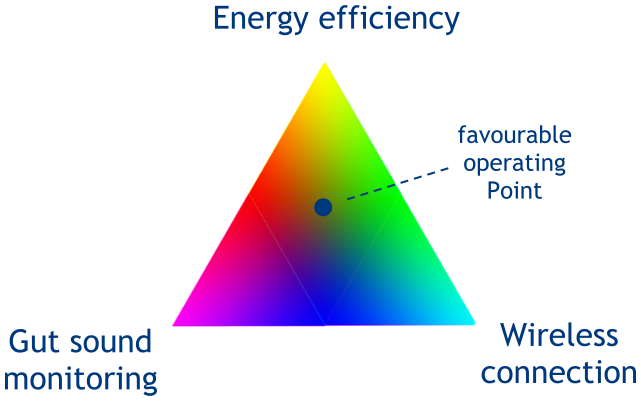
\includegraphics[width=0.8\textwidth]{Images/design_challenges}
\caption{System design challenges}
\label{fig:design_challenges}
\end{figure}

Figure \ref{fig:design_challenges} shows one  way to visualize this three-way tradeoff - it is impossible to design a system with a very high energy efficiency that performs high quality gut sound monitoring and transmits data wirelessly at the same time, because the design space doesn't contain an operating point for this configuration. 

An example for this is our goal to be very energy efficient, because battery life is highly important for mobile devices. Aiming for high energy efficiency puts a constraint on the available choices for a wireless connection, because many wireless protocols are rather energy hungry. At the same time it limits the amount of processing that can be done on the monitoring device, because a busy processor consumes a lot of energy and the aim is to keep the processor sleeping for as long as possible. The cases where sending a larger block of data over wireless is actually more energy-efficient than processing the data on the monitoring device and sending less data over wireless are good illustrations of this tradeoff. 

In order to come up with a design solutions for the main challenges a design space analysis was conducted, where the team attempted to find an operating point close to the center of the design space triangle. The tradeoffs that were taken into consideration will be explained in more detail in the following paragraphs.  

Energy efficiency and the inconveniences caused by the lack of it were mentioned before. One major design goal is a long battery runtime which can only be achieved if every component of the monitoring device is optimized for low power usage. This limits the available choices for the wireless communication protocol and also puts a constraint on the amount of data processing that can be done on the monitoring device.
 
Wireless communication between the monitoring device and the base station is another important issue. A wireless protocol solution which satisfies the bandwidth requirements (audio transmission) while consuming only very little energy is desired. 

Gut sound monitoring is the last of the main design challenges. To be able to do any kind of examination based on the audio data, the length of the recording has to be in the minute range. This requires a wireless protocol with a bandwidth that allows to transmit the data in a reasonable amount of time and limits the processing that can be done during recording because the processor should not be involved in the optimal case.

\section{Proposed System}
The system that we propose to tackle the design challenges is a distributed system, consisting of wireless monitoring devices optimized for low energy consumption and stationary base station that collects data from monitoring devices and presents it to the user over a web interface. 

This design stands in contrast to the first proposal for the system design in which there is no distinction between monitoring station and base station and the user interacts directly with the system over a wireless protocol commonly available in handheld devices and laptops (Bluetooth) or connects to the device via USB. We realized early that this design was suboptimal, as it’s neither scalable nor suited for running on battery power over an extended period of time as Bluetooth is an energy hog and the data processing cannot be offloaded but has to be performed on the device itself.

Separating the roles in the system into distinct devices gives the possibility to design nodes that are optimized for their role in the overall system, which is especially important in this case, as  one of the key focus areas of this project is to build a battery powered device with a long battery runtime. This can only be achieved if the goal is kept in mind during all stages of the design - from the selection of the used components to the design of the system software.

\subsection{Distributed system}
\begin{figure}[htb]
\centering
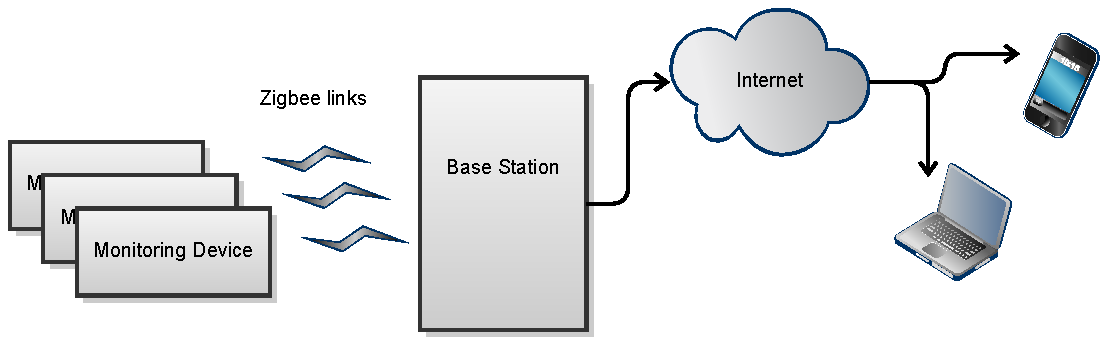
\includegraphics[width=\textwidth]{Images/gdp_system_block}
\caption{Block Diagram: Distributed system}
\label{fig:block_system}
\end{figure}

Figure \ref{fig:block_system} shows  block diagram of the proposed system consisting of multiple monitoring devices and a base station. 
The base station is a stationary device connected to a constant energy source. It provides the network for wireless communication between monitoring devices and the base station. Measurement data from monitoring devices is received over this network, and stored in an internal database. It serves as a common access point for users to retrieve the collected data from multiple monitoring devices and provides easy access from a wide range of devices by presenting the collected data via a web interface.

The monitoring device is a portable battery powered device that can be attached to horses with a strap, and features a range of sensors, a digital stethoscope and means for temporal data storage. The collected data is transferred periodically to the base station, or preserved for later transmission in the local data storage, if the base station is out of reach.

Data access is provided to the user by the base station over a web-interface that displays the collected data and allows the user to download a database for detailed analysis. The audio recordings are stored on an flash memory card in the monitoring devices, and only transferred to the base station of the user requests a data transfer.

\subsection{Wireless connection between nodes}
\label{sec:wireless_connection}
When the decision was made that a distributed system will be developed this also meant that the collected data has to be transmitted wirelessly to the base station, which is as not straightforward as it sounds, given the constraints imposed by the other main challenges that were discussed in section \ref{sec:design_challenges}.

A wireless protocol that had very low energy consumption while offering enough bandwidth to transfer audio signals and supported a range of around 100m was required to adhere the project goals.

In the end the choice fell on the ZigBee protocol, which came closest to fulfilling our feature wish list. The main factors that influenced our decision were
\begin{itemize}
\item Range: up to 100m
\item Power consumption: very low, as it is specifically designed for low-power applications
\item Bandwidth: up to 250kB/s
\item Complexity: easy to setup and use
\end{itemize}

The system is designed in such a way, that monitoring devices have to establish a connection with the base station if they want to transmit data. For energy saving reason, the monitoring devices put their ZigBee modules to sleep when they are not actively transmitting data. This means that the base station cannot send data (commands/requests) to the monitoring devices at arbitrary points of times. It has to wait until a monitoring device connects to the base station before it can dispatch messages. 


\chapter{Hardware Subsystems}
\label{chap:hardware_subsystems}
In this chapter building blocks of the proposed system, each of which were separately prototyped to allow a good degree of parallelisation, are described. The driver software that makes each unit functional is also mentioned. We discuss the top-level software that brings these blocks together into a functional system in the chapter \ref{chap:system_software}.


\section{Monitoring Device}
The monitoring device is designed to be a simple device that acquires data from the sensors, stores the data and sends it to the base station when the ZigBee link is available. It contains a microcontroller, a set of sensors for data acquisition, a memory card to store data and a ZigBee module for wireless communications.

\begin{figure}
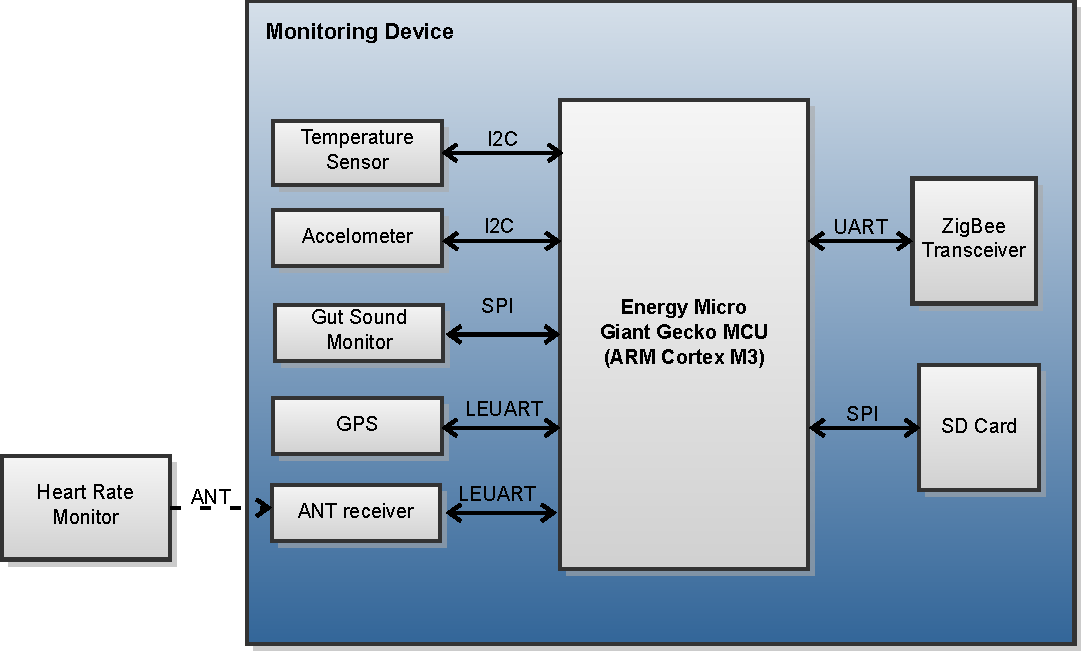
\includegraphics[width=\textwidth]{Images/MonitoringDeviceBlockDiagram}
\caption{Block Diagram: Monitoring Device}
\label{fig:monitoring_device_block}
\end{figure}

The following sub-chapters will discuss the implementation of each subcomponent of the monitoring device, shown in Figure \ref{fig:monitoring_device_block}, together with the properties of the hardware and how they map to the requirements of the project.


\subsection{The Microcontroller (MCU)}
As the monitoring device is required to be a battery-operated system that contain a number of diverse peripherals, choosing the right central processing unit was essential. Reviewing existing microcontrollers in the market we opted for an EFM32 Giant Gecko microcontroller from Energy Micro, which contains a 32-bit ARM Cortex M3 core and a set of on-chip peripheral interfaces. The EFM32 was considered to be a good match for the requirements, as shown in the table \ref{tab:microcontroller_properties}.

\begin{table}
\begin{tabular}{|m{0.45\textwidth}|m{0.45\textwidth}|}
\hline 
	\textbf{Device Properties} & 
	\textbf{Corresponding Requirements} \\ 
\hline
	\begin{itemize}
	\item up to 48 MHz high-frequency operation
	\end{itemize}&
	\begin{itemize}
	\item handle large data volumes from multiple sensors and audio
	\end{itemize} \\
	
\hline
	\begin{itemize}
	\item different levels of sleep
	\item fast wake up time (2 $\mu S$)
	\item 32.768 kHz low-frequency operation for sleep modes
	\item low energy periphals operational even in deep sleep modes
	\item DMA and PRS (Peripheral Reflex System) for acquiring data without waking up the processor core
	\end{itemize} &
	\begin{itemize}
	\item long battery life
	\item long periods of sleep
	\item low energy periodic sampling
	\end{itemize} \\
\hline
	\begin{itemize}
	\item 128 KB SRAM, 1MB flash memory
	\end{itemize} &
	\begin{itemize}
	\item ease of development
	\item suitable for overheads introduces by C++
	\end{itemize} \\
\hline
	\begin{itemize}
	\item 3 x USART with I2S support
	\item 2 x low energy UART (LEUART)
	\item 2 x I2C interfaces
	\end{itemize} &
	\begin{itemize}
	\item various interfaces for peripherals and sensors
	\end{itemize} \\
\hline
	\begin{itemize}
	\item 64-pin TQFP package
	\end{itemize} &
	\begin{itemize}
	\item ease of soldering (lack of BGA mounting equipment)
	\end{itemize} \\
\hline 
\end{tabular} 
\caption{Microcontroller properties}
\label{tab:microcontroller_properties}
\end{table}

Some of the more specialized properties of the microcontroller which give it advantages for our solution are briefly explained below:

\subsubsection*{Energy Modes and Low Energy Peripherals} The EFM32 microcontrollers offer four levels of sleep, and some special peripherals (called low energy or LE peripherals) that are able to keep functioning even in deep sleep modes. Of particular interest to us are the LEUART interface which while deeper sleep modes provide more energy savings, it also becomes more difficult to implement a reasonable level of active functionality. An overview of sleep modes and available peripherals in each is presented in table \ref{tab:microcontroller_modes}.

\begin{table}
\centering
\begin{tabular}{|l|l|m{6cm}|}
\hline
	\textbf{Energy Mode}&
	\textbf{Power consumption}&
	\textbf{Description}  \\ 
\hline
	EM0 &
	$200 \frac{\mu A}{MHz}$ &
	All peripherals active, CPU core active  \\ 
\hline
	EM1 &
	$50 \frac{\mu A}{MHz}$  &
	All peripherals active, CPU core sleep  \\ 
\hline
	EM2 &
	$1.2 \mu A$  &
	LEUART, LETIMER, I2C, RTC, LCD, PCNT, LESENSE, ACMP, OPAMP, USB active  \\ 
\hline
	EM3 &
	$0.9 \mu A$  &
	Full CPU and RAM retention, asynchronous external interrupts and I2C can wake up the device   \\ 
\hline
	EM4 &
	$20 nA$  &
	All functionality off, GPIO pin retention and wake up from GPIO interrupt  \\ 
\hline 
\end{tabular} 
\caption{Microcontroller energy modes}
\label{tab:microcontroller_modes}
\end{table}

\subsubsection*{Peripheral Reflex System (PRS)}
Using a signal producers - signal consumers concept, it is possible to make peripherals in the EFM32 microcontroller directly communicate with each other without involving the CPU. Thus, an action can be automatically triggered in peripheral A when an event occurs in peripheral B. This can be used to achieve more stable time-critical operations and less software overhead, as well as saving energy since the CPU does not have to intervene.

\subsubsection*{Direct Memory Access (DMA)} DMA allows blocks of data to be moved between RAM and peripherals without CPU intervention, thus freeing CPU resources and allowing longer periods of sleep, as well as offering stable high bandwidth memory transfers for operations like audio acquisition.

Further details of how the PRS, DMA and different sleep modes are used in the system is provided in chapter \ref{chap:system_software}


\subsection{Heart Rate Monitor (HRM)}
The heart rate is an important vital sign for any health monitor, although designing a portable device to acquire heart rate is not a trivial task. The issues of electrode placement, filtering out changes due to subject movement and processing the resulting ECG signal are challenging and time consuming. Another challenge specific to our project is acquiring both gut sounds and the heart rate; it is not possible to reliably acquire both signals from the same physical location so a wired microphone or electrode would have to be attached to the horse. 

To address both these problems, we chose an ANT wireless module that can be used with any ANT+ compatible heart rate chest strap, commercially available for both horses and humans. Attaching a separate heart rate monitor chest strap and transmitting heart rate information wirelessly solves the problems mentioned above and brings the additional advantage of making the system usable for humans.

\begin{table}
\centering
\begin{tabular}{|m{0.45\textwidth}|m{0.45\textwidth}|}
\hline 
	\textbf{Device Properties} &
	\textbf{Corresponding Requirements}  \\ 
\hline
	low power  &
	low energy periodic sampling  \\ 
\hline
	simple UART interface &
	ease of development \\
\hline
	can pair with a particular ANT+ HRM chest strap &
	monitoring multiple horses \\
\hline 
\end{tabular} 
\caption{Heart Rate Monitor properties}
\label{tab:hrm_properties}
\end{table}

\textbf{Interface:} \TODO{rephrase} LEUART with configurable baud rate, not lots of data so high BR does not make sense

\textbf{Driver:}
\TODO{talk about ANT driver:} LEUART, configure \& open network with wildcard id, establish connection \& rcv heart rate. search timeout \& disconnection \& pairing.


\subsection{Temperature Sensor}
5.1.3 Temperature Sensor
As with many other warm-blooded animals, body temperature can be a valuable tool for diagnosis in horses. While electronic temperature measurements are usually done by an element that comes into physical contact with the subject, doing temperature measurements in this manner on a moving horse is likely to cause fluctuations in the read values. This is the reason we preferred to use a contactless temperature sensor for our implementation. 

\TODO{Fix this} TMP006 [http://www.ti.com/lit/ds/symlink/tmp006.pdf] which is a contactless infrared temperature sensor from Texas Instruments was chosen for the project. 


\begin{table}
\centering
\begin{tabular}{|m{0.45\textwidth}|m{0.45\textwidth}|}
\hline 
	\textbf{Device Properties} &
	\textbf{Corresponding Requirements}  \\ 
\hline
	low power:
	\begin{itemize}
	\item 240-325 $\mu A$ during active conversion
	\item 90 $\mu A$ in sleep mode 
	\end{itemize}  &
	low energy periodic sampling  \\ 
\hline
	contactless temperature measurement &
	portable, mobile monitoring device \\
\hline
	passive (slave) device over I2C bus &
	advantageous for a system with lots of sensors, will not send and generate interrupts unless requested \\
\hline 
\end{tabular} 
\caption{Temperature Sensor properties}
\label{tab:temp_sensor_properties}
\end{table}

\textbf{Interface:} The TMP006 offers an SMBus-compatible interface, which is interoperable with I2C and was connected to the I2C interface on the microcontroller. Controlling device functionality and accessing measurement data is done via “write to register” and “read from register” commands. 

\textbf{Driver:} Our TMP006 driver configures device sleep state and conversion rate by writing values to the appropriate registers (TODO insert reference to TMP006 datasheet). The temperature measurement is provided by reading the two registers which contain the voltage generated by the thermopile and the die temperature. The temperature of the object can be calculated from these two data. However this calculation involves heavy floating point arithmetic and it is rather inefficient on the microcontroller. Therefore, the “raw” temperature reading consisting of these two values is not processed on the monitoring device any further but sent to the base station, whose ARM11 core is much more efficient at handling this calculation. 


\subsection{GPS}
A popular peripheral in many consumer devices today, GPS (Global Positioning System) allows tracking the position of a sensor in terms of global coordinates. While not immediately useful for clinical purposes, the ability to track the location of horses on this level can be beneficial if recording of movements or activity recognition [TODO ref High Classification Rates for Continuous Cow Activity Recognition using Low-cost GPS Positioning Sensors and Standard Machine Learning Techniques.]  is desired over a longer period of time in a larger area (for free-roaming horses or other animals). 

Commercial drop-in GPS modules are available and straightforward to use, but power consumption while searching limits the possibilities for a battery-powered system with energy efficiency focus. We chose a UP500 GPS module from Fastrax \footnote{\url{http://www.fastraxgps.com/products/gpsantennamodules/500series/up500/}}
for our project. UP500 is a GPS receiver module with embedded antenna offered in a very small package, and offers significant power savings by providing an option to save satellite data to RAM while still being able to wake up from this state and get a position fix within a few seconds (called a “hot start”). 

\textbf{Interface:} The UP500 with the microcontroller via UART and uses a baud rate of 9600 (8 data bits, 1 stop bit, no parity). The Low Energy UART (LEUART) peripheral on the EFM32 was used for this connection, which can receive data at low baud rates even while in deep sleep mode (down to EM2).

\textbf{Driver:}
\begin{itemize}
\item{Data acquisition:}
For maximum energy efficient operation, the GPS driver configures the GPS module to use LEUART interface with DMA. DMA transfers incoming NMEA messages into a fixed size buffer when new data is available. The LEUART module is configured to generate an interrupt whenever it receives the newline character (0x0A). Since every NMEA message ends with a newline, an interrupt is generated every time a complete message is received, and the contents of the DMA buffer are copied to another internal buffer for processing at a later time.

\item{Parsing NMEA messages:} \TODO{} simple string parsing, comma delimited fields,NMEA message types GPRMC and GGPA are handled
\begin{itemize}
\item output: valid position fix, latitude and longitude
\end{itemize}

\item{Sleep mode:} The UP500 does not have a dedicated sleep pin, but once satellite data has been acquired it is possible to put the device into a sleep-like mode where the power consumption becomes quite low. This is done by turning off the power to the $V_{cc}$ supply pin, while keeping the $V_{bat}$ supply pin active. By keeping ephemeris data in RAM, the GPS is thus able to establish the position quickly when the $V_{cc}$ supply is reinstated. Switching the $V_{cc}$ supply is done via a transistor attached to a GPIO pin, consult section \TODO{} for more details.
\end{itemize}


\subsection{Accelerometer}
In addition to the location tracking capabilities provided by the GPS, it can be useful to measure smaller movements with higher precision. Accelerometer data collected in this manner can be used to detect lameness and injuries. The particular challenge for using an accelerometer in our system was the high sampling rate necessity - the collected acceleration data will not be useful at low sampling rates\footnote{\TODO{find a good citation for this}}. While high sampling rate itself is not a problem for the EFM32 microcontroller, it conflicts with low energy periodic sampling - if the microcontroller has to poll the device for new data at a high frequency, it will not have a lot of time to sleep. An accelerometer that contains an on-chip buffer can remedy this problem; the MCU can simply enable sampling, go back to sleep, and wake up when the desired number of samples have been acquired to read them from the sensor’s own buffer.

We chose the 3-axis  ADXL350 \footnote{\url{http://www.analog.com/en/mems-sensors/mems-accelerometers/adxl350/products/product.html}} digital accelerometer from Analog Devices for the project. It is capable of measuring acceleration in the ranges ±1g, ±2g, ±4g or ±8g and it has a FIFO buffer which allowed us to implement the scheme discussed in the previous paragraph.

\begin{table}
\centering
\begin{tabular}{|m{0.45\textwidth}|m{0.45\textwidth}|}
\hline 
	\textbf{Device Properties} &
	\textbf{Corresponding Requirements}  \\ 
\hline
	.
	\begin{itemize}
	\item Ultralow power: $45 \mu A$ in measurement mode and $0.1 \mu A$ in standby mode
	\item FIFO buffer can hold up to 32 samples
	\end{itemize} &
	low energy periodic sampling  \\ 
\hline 
\end{tabular} 
\caption{Accelerometer Sensor properties}
\label{tab:accelerometer_properties}
\end{table}

\textbf{Interface:} Similar to the TMP006, the ADXL350 is interfaced through the I2C bus; controlling device functionality and accessing measurement data is done via “write to register” and “read from register” commands. 

\textbf{Driver:} ADXL350 supports both SPI and I2C interfaces. In this project, it is used in I2C mode. The accelerometer offers a 32-level FIFO which has 4 modes of operation configured by control registers: Bypass, FIFO, Stream and Trigger Mode. The driver configures the FIFO in Bypass Mode which disables the FIFO. The 4-phase scheme (\TODO{I don’t know how to refer this}) is applied for power management. 


\subsection{Gut Sound Monitoring}
\TODO{Insert content from document}


\subsection{Data Storage}
Relatively low throughput of ZigBee link between the base station and the monitoring devices makes gut sound streaming inconvenient considering the amount of audio data produced. \TODO{}: Here we can quote amount of audio\ldots. One possible solution was to stream a smaller amount of data and record a longer audio data into an on-board storage element. Therefore, a microSD card was incorporated into the system. 

SD Card solution provides two other benefits to the system besides complementing the limits of wireless streaming. The SD Card can be used to save data collected from all sensors when the base station is out of reach. This way the sensor data is not lost when there is no connection between the base station and the monitoring device. Also, it can be removed by the user to copy the data when needed, since a wide range of devices are SD card compatible.  

SD Cards are based on flash memory technology. They support 3 communication modes: SD 1-bit, SD 4-bit and SPI mode\footnote{\url{http://alumni.cs.ucr.edu/~amitra/sdcard/Additional/sdcard_appnote_foust.pdf}}. 

In SD 1-bit mode, the data is transferred over 1-bit wire in a synchronous serial fashion. SD 4-bit protocol is the same as SD 1-bit protocol except that bulk data transfer is done over 4-bit bus. SD 4-bit mode can provide speed benefits over SPI mode. However it is not recommended in software solutions since it requires CRC calculation for each of the four wires and may result in a big computational effort. Also, accessing the complete SD Card Specifications to build an SD standard device requires licenses from SD Card Association\footnote{\url{https://www.sdcard.org/developers/howto/}}. Therefore, in this project, the card is used in SPI mode. 

\TODO{Check this:}TODO: Check this (“If your company is planning to manufacture or have manufactured SD standard devices  (eg. cell phones, cameras or computers) or SD ancillary products (eg. adapters or SD I/O cards), your company is required to:”, I think using SD bus is “manufacturing an SD standard device”)

To implement microSD prototype system, an existing FAT file system and a low-level disk interface module were used. The card was connected to one of the SPI interfaces of the microcontroller. MicroSD cards support up to 208 MHz clock frequency [TODO citation]. The clock system of the Energy Micro microcontroller allows maximum SPI bit rate to be at half speed of the source clock in master mode \TODO{Citation: EFM32\_GG Ref}. Theoretically, SPI clock can be up to 24 MHz when the source clock is set to 48 MHz. However, there is an upper speed limit caused by delays of inputs and outputs of the microcontroller which is not specified by the manufacturers\footnote{\url{http://forum.energymicro.com/topic/288-microsd-card-spi-baudrate/}}. Our microSD driver sets SPI clock speed at \TODO{X} Mhz at which it operates safely.   


\section{Wireless Interfaces}
\subsection{Data transmission - ZigBee}
Because of the decision to design a distributed system that transmits data wirelessly between monitoring devices and the base station, it was necessary to come up with a customized stable wireless communication path. As discussed in section \ref{sec:wireless_connection} the ZigBee protocol was chosen for the wireless communication between the base station and the monitoring devices.

As ZigBee is an open standard there are multiple vendors offering devices implementing the protocol. Because of the widespread use in homebrew electronic projects we decided to use devices by Digi which offer a whole ZigBee based product line called XBee. 

The main advantage was that the prototyping could be sped up due to availability of breakout boards, and XBee to USB converters (figure \ref{fig:xbee_prototyping_interfaces}). This allowed to implement, test and debug the software module for wireless communication on a normal computer before porting it to the embedded system.

\begin{figure}

\includegraphics[width=\textwidth]{Images/dummy}
\caption{XBee prototyping interfaces}
\label{fig:xbee_prototyping_interfaces}
\end{figure}

The wireless software module uses an existing open-source software library to handle the low level communication with the XBee hardware, and adds an object oriented interface as well as utility classes that allow to use and control the wireless connection at a high abstraction level. More details on the design of the software module are given in section \ref{sec:wireless_communication_software}


\subsection{Communication with Heart Rate Monitor - ANT}
\TODO{Not yet written}


\section{Base Station}\begin{figure}
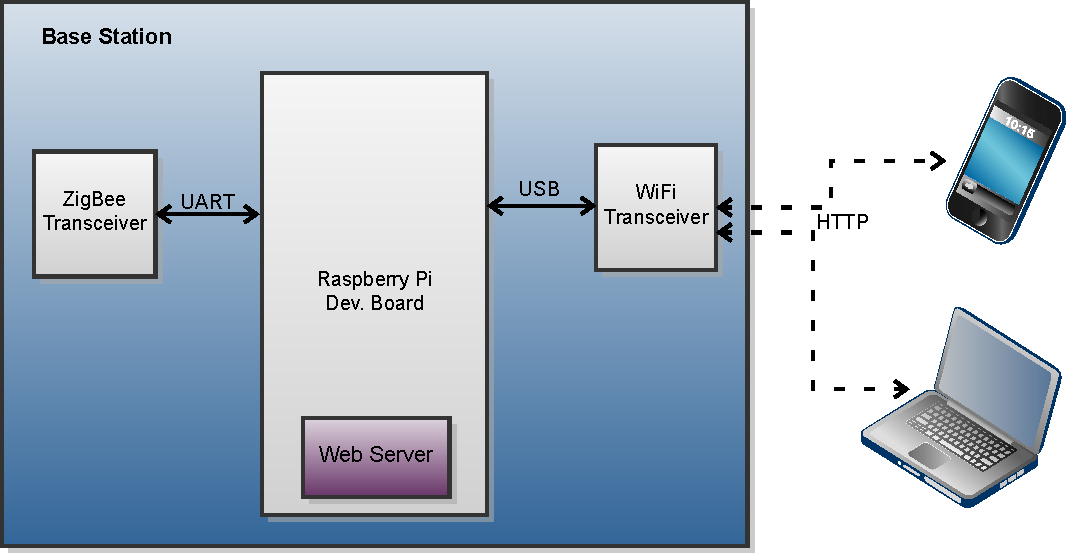
\includegraphics[width=\textwidth]{Images/BaseStationBlockDiagram}
\caption{Block Diagram: Base Station}
\label{fig:block_base_station}
\end{figure}

The base station collects data from the monitoring devices, stores this data in a database and makes it available and via a webserver running on the device itself. The advantage of using a website to provide access to the collected data is the support for a variety of devices with web access. In addition, it compensates disadvantage of the short range low data-rate ZigBee connection making the data accessible from anywhere.  


\subsection{Hardware platform}
The base station acts as a bridge between the “proprietary” monitoring stations and the end user, who wants an easy way to access the data that is collected by the system. The challenges for the base station lay mainly in the software domain. The only requirements that exist for the platform is that it has a to be able to interface an XBee device, a WLAN transceiver and provide means for mass data storage. 

For these reasons the decision was made, that an existing hardware platform would be used to implement the base station. The choice fell on the Raspberry Pi which provides a number of positive implications that are listed in table \ref{tab:raspberry_capabilities}.


\subsection{Raspberry Pi}
\begin{table}
\centering
\begin{tabular}{|l|m{6cm}|}
\hline
	Price &
	35£   \\ 
\hline
  	Software &
  	Raspberry can run a Debian based distribution, which gives access to a huge set of open-source programs and libraries  \\ 
\hline
	Connectivity &
	Features an ethernet port, USB host capabilities and HDMI output that could be used to attach a display to the base station  \\ 
\hline
	Extendability / GPIP  &
	20 GPIO pins, support for I2C, SPI, Serial  \\ 
\hline
	Storage &
	SD-Card slot with support for cards up to 64GB  \\ 
\hline
	Power consumption &
	Very low, between 1.5 and 2 Watt \\ 
\hline
 	Size &
 	Very small form factor (85.6mm x 56mm)  \\ 
\hline 
\end{tabular} 
\caption{Raspberry Pi capabilities}
\label{tab:raspberry_capabilities}
\end{table}

In summary it can be said that the Raspberry Pi is very well suited for rapid development of embedded systems, as long as they are not supposed to run on battery. It offers the convenience of developing software in a Linux environment while giving direct access to low level I/O capabilities for interfacing custom hardware.

\subsection{XBee}
As mentioned in section \ref{sec:wireless_connection} we use of XBee devices to implement the ZigBee network for data transmission between monitoring devices and the base station. These devices are widely-used in (homebrew) electronic projects, and they have the advantage that a Raspberry compatible XBee adapter board already exists. The adapter goes by the name of Slice of Pi and is shown in figure \ref{fig:xbee_prototyping_interfaces}.

\chapter{System Software}
\label{chap:system_software}
Having discussed how the functionality of each subsystem is implemented in chapter \ref{chap:hardware_subsystems} we now provide a description of the software that brings these subsystems together into a complete system. 


\section{Monitoring Device}
For the reasons discussed in section \ref{sec:design_challenges}, the functionality of the monitoring device is kept simple and can be summarized as gathering data from the sensors, storing the data offline in the SD card when the ZigBee wireless connection is not available, and sending the gathered data to the base station. Figure \ref{fig:dataflow_monitoring_device} illustrates the data flow on the monitoring device.

\begin{figure}
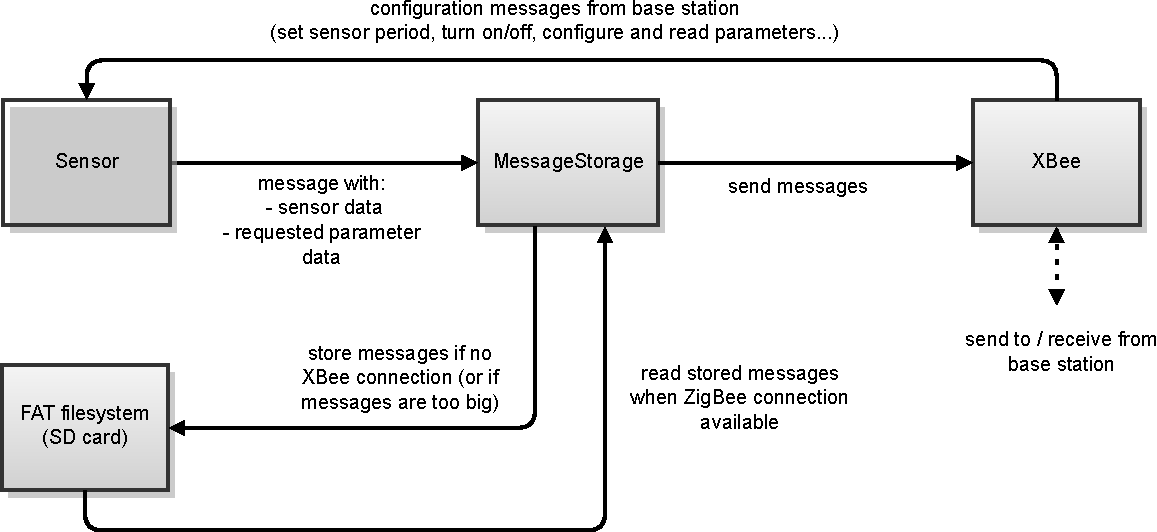
\includegraphics[width=\textwidth]{Images/monitoringdevice_dataflow}
\caption{Monitoring Device: dataflow}
\label{fig:dataflow_monitoring_device}
\end{figure}

Furthermore, to keep the energy efficiency focus, this data flow has to be implemented using periodic sampling and automated data acquisition whenever possible. The following subsections will describe these implementation details for the system software on the monitoring device.

\subsection{Development Paradigm and Environment}
The monitoring device software was developed using a mix of C++ and C, with IAR Embedded Workshop for ARM as the development environment. Using this mix of object-oriented and procedural programming paradigms, we aimed to achieve the best of both worlds - C++ classes were created to take advantage of polymorphism and encapsulation where possible, while pure C was used in places where small and efficient functions (e.g for handling DMA callbacks or audio-related tasks) were needed.

The choice of object-oriented paradigm (OOP) and C++ may be considered unusual for a highly integrated embedded system, but we considered the advantages to outweigh the penalties for our project. The 128 KB of RAM is enough to compensate for overheads introduced by C++, and sensor drivers involve handling tightly coupled data and functionality, which is suitable for modelling them as objects. Additionally, deriving all sensor implementations from the same Sensor base class allowed the integration of sensors into the final system in a plug-and-play manner, since they all share the same interface.



\subsection{Low Energy Periodic Sampling, Sensor Interface and Drivers}
\begin{figure}
\centering
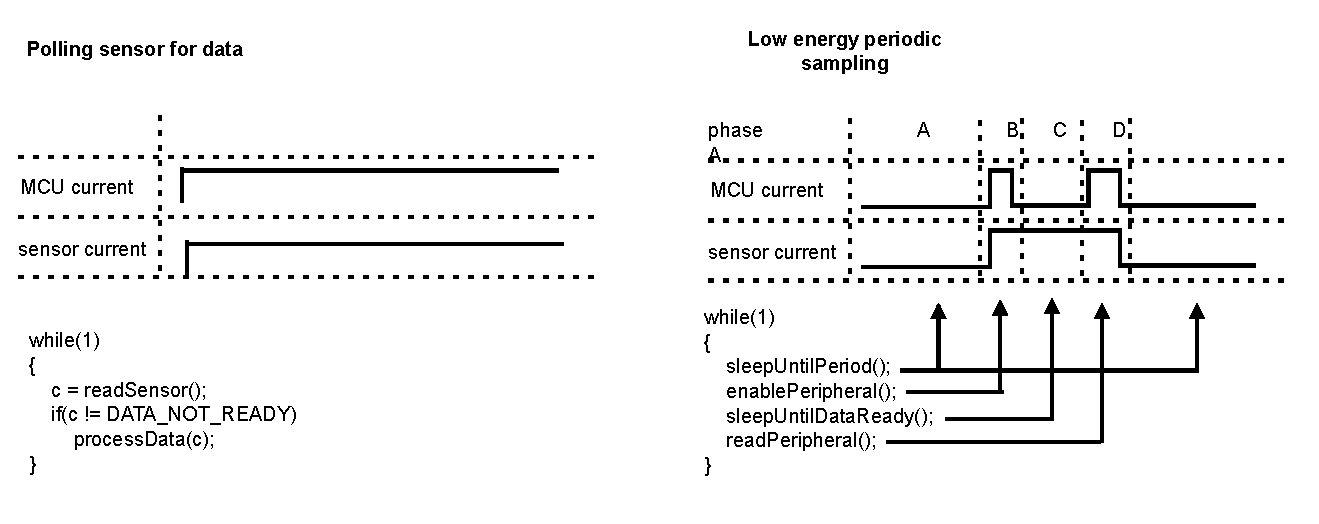
\includegraphics[width=\textwidth]{Images/sampling_comparison}
\caption{Sampling comparison}
\label{fig:sampling_comparison}
\end{figure}
We now discuss our definition of low energy periodic sampling for the monitoring device, and the relevant OOP basis we constructed towards its implementation. The basic idea behind low energy periodic sampling is that a receiving a continuous stream of data from all the sensors all the time is not necessary for monitoring purposes is unnecessary. Depending on the sensor type, receiving a sample with a period of tens of seconds, perhaps minutes can be sufficient for analysis. In this case, since the sensor and the microcontroller are not required to be active all the time, significant energy savings can be achieved by putting them into sleep mode until the start of the next period. This scheme can be further extended by introducing an additional period of sleep for the microcontroller after it awakens the sensor and waits for data. An illustration of how this compares with the continuous polling approach can be found in figure \ref{fig:sampling_comparison}, with a more detailed explanation of the power management phases in table \ref{tab:power_phases}. It can be seen that the low energy periodic sampling offers much less current consumption compared to polling.

\begin{table}
\centering
\begin{tabular}{|l|m{1.5cm}|m{1.5cm}|m{2.5cm}|m{4.5cm}|}
\hline
	\textbf{Phase}  &
	\textbf{MCU state}  &
	\bfseries Sensor state  &
	\textbf{Duration}  &
	\textbf{Description}  \\ 
\hline
	Phase A &
	asleep  &
	asleep  &
	as desired  &
	both sleepig and waiting for next sampling period to start  \\ 
\hline
	Phase B &
	awake  &
	awake  &
	MCU dependent (wakeup time)  &
	microcontroller wakes up peripheral, peripheral starts sampling  \\ 
\hline
	Phase C &
	asleep  &
	awake  &
	sensor dependent (sampling rate)  &
	microcontroller sleeps while waiting for peripheral to complete sampling  \\ 
\hline
	Phase D &
	awake  &
	awake  &
	bus dependent (data read speed)  &
	data ready, microcontroller reads data from peripheral, then go back to Phase A   \\ 
\hline 
\end{tabular}
\caption{Periodic sampling power phases}
\label{tab:power_phases} 
\end{table}

This energy saving scheme can be applied to any sensor or peripheral that supports sleep mode. As we chose all only sleep-supporting sensors for our implementation, we were able to identify a set of properties and functions common to all sensors which forms the Sensor base class. The properties and methods defined in the class are listed in section \ref{list:sensor_interface}. 

To summarize, the \textit{setSleepState} function is used to put the sensor to sleep and wake it up, the \textit{sampleSensorData} acquires data from the sensor into internal buffers, and \textit{readSensorData} gives access to the data in the internal buffers wrapped in a \textit{SensorMessage} structure (described in section \ref{sec:message_types}). Individual sensors drivers are derived from this base class and implement the common methods in their specific way, as described in chapter \ref{chap:hardware_subsystems} 


\subsection{Timekeeping and Alarm System}
\label{sec:timekeeping}
Timekeeping and Alarms System
To implement the periodic sampling scheme discussed in the previous section, it is necessary to keep track of real time and trigger an alarm when an action (such as waking up the sensor from sleep) is needed. The same implementation can be used to provide small fixed-length blocking delays in code, which are useful in the driver implementations.

The EFM32 has a dedicated  Real Time Counter (RTC) peripheral which makes this implementation easy, but the challenge is once again doing this in an energy efficient way. For example, it is possible to configure a system tick that wakes up the MCU every millisecond and updates an internal counter, but waking up every millisecond is very inefficient in terms of energy. Most of the time, we require periodic alarms that are generated in the range of seconds for the low energy periodic sampling scheme. This means timer tick interrupts that wake up the processor every second is enough for our purposes.

To our convenience, the EFM32 RTC peripheral can be kept active down to deep sleep (mode EM2) by using the low frequency oscillator (\TODO{} refer to section TODO section:pcboscillators for details) and be configured to generate interrupts only when the tick counter reaches a certain value. This allows us to do timekeeping at a very low energy cost and generate alarms with second-precision. Additionally, it is still possible to generate millisecond-accurate interrupts using the secondary compare register when needed.

This functionality is encapsulated inside the \textit{AlarmManager} class, which offers easy energy-efficient timekeeping and periodic alarm generation functionality. It can be used to generate periodic or single-shot alarms that become triggered after a given number of internal ticks. The triggered alarm executes a callback function specified at the alarm creation time. The internal tick period itself is configurable from milliseconds to hours. The class also supports an energy efficient delay function that can be used to create a blocking delay with millisecond resolution while putting the MCU to sleep in the desired mode. Finally, the class exposes the number of seconds and/or milliseconds elapsed since the start of monitoring device operation, which is used to generate timestamps for the sensor messages that are sent to the base station \TODO{:} connect this to appropriate section about relative timekeeping.

One final issue regarding timekeeping is persistence across reboots. The monitoring device may stop and restart execution after some time due to the battery running out. To keep the integrity of timestamps, the RTC second counter is regularly backed up to the SD card and re-read upon reboot.

\subsection{Task Scheduling and Sleep Management}
While it is intuitive to model the functionality that reads data from each sensor as a separate task and then use a real-time operating system to execute these tasks concurrently, we preferred not to use an RTOS as they typically use high-frequency system tick interrupts to do task scheduling and dispatching, and a high frequency system tick is not compliant with our low energy goals due to the reasons explained in the previous section. There are RTOS ports for EFM32 that avoid this, Therefore, we rely on the periodic alarms generated by the AlarmManager to trigger sensor readings.

The problem with this approach is the fact that the alarm handler callback functions are executed inside the interrupt context. If the alarm handler takes a long time to execute (for example, read a large amount of data from the sensor) this will result in staying in the interrupt context for a long time. Even though the EFM32 supports nested interrupts, it is considered to be bad practice to have big interrupt service routines since it can introduce instabilities into the system. Our solution to the problem was to adopt the deferred procedure call (DPC) approach for periodic readings. Illustrated in figure \ref{fig:deferred_reading} a DCP shifts the execution of time consuming data acquisition functions to the main context instead of doing them inside the interrupt context..

\begin{figure}
\centering
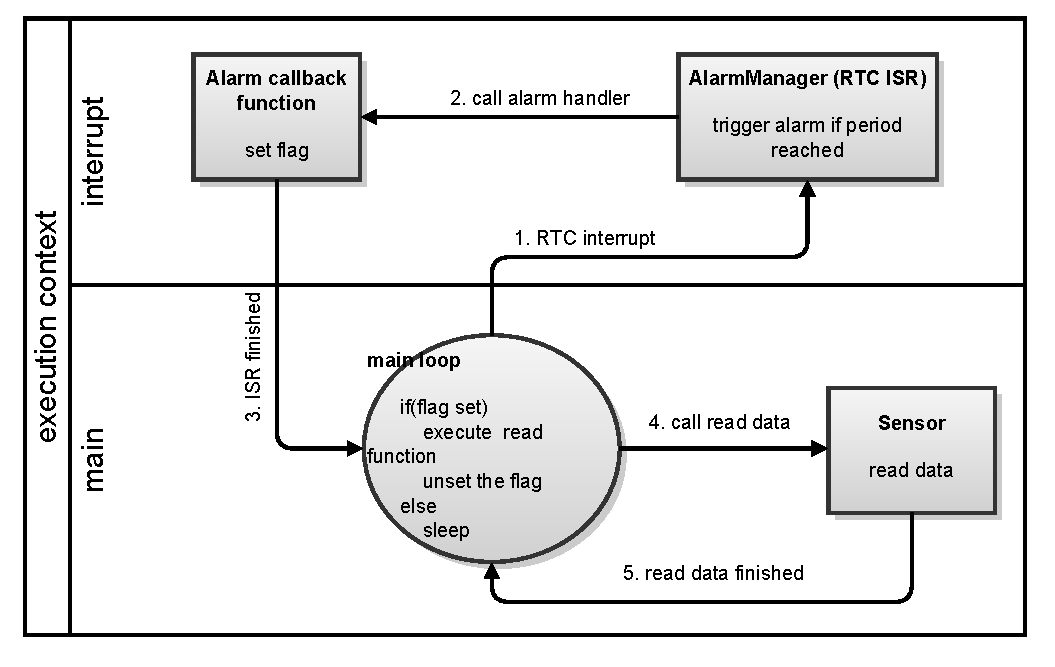
\includegraphics[width=\textwidth]{Images/deferred_reading}
\caption{Deferred reading}
\label{fig:deferred_reading}
\end{figure}

In this scheme, the interrupt handlers do not do any processing beyond taking actions so that received data is not lost but buffered in memory. The ISR then sets a flag indicating that the corresponding handler task should be executed. When the control returns to the execution loop, it checks each flag in order of decreasing task priority, executes the task if its flag is set and clears the flag afterwards. The processor then goes to sleep until the next interrupt.

Since the order of checking the task flags determine the execution priority and because the scheme is not preemptive, the tasks must be designed to be short (i.e not block execution for long periods). Not observing this principle can cause a big backlog of tasks to be executed and leave the processor no time to sleep.

A final consideration is the handling of asynchronous interrupts during sleep. This scheme is dependent on interrupts from hardware waking up the MCU from sleep, so care must be taken to ensure that the sleep level chosen will not disable the hardware that will generate the interrupts. 

\subsection {Message Storage System}
In order not to lose any acquired samples when the wireless connection to the base station is not available, it is necessary to save the samples on persistent storage. The project utilizes an SD card for this purpose, as described in section \ref{sec:data_storage}. This chapter focuses on the software component which abstracts the data storage for the convenience of sensor systems.

It is possible to model the message storage requirements of the monitoring device on two levels: in main memory and in SD card. Sensor readings are placed in the main memory when retrieved and stay there until they either get sent to the base station or become saved to the SD card. When the base station connection becomes available, the messages stored in the SD card are read out and sent first.Therefore, if we view the sampled data as a queue of messages, the way the rest of the system interacts with this queue is actually irrelevant whether the data is stored in memory or on disk. 

\begin{figure}

\includegraphics[width=0.5\textwidth]{Images/dummy}
\caption{Class Diagram: MessageStorage}
\label{fig:class_message_storage}
\end{figure}

Our \textit{MessageStorage} class takes advantage of this and offers a simple enqueue-dequeue interface to the rest of the system. Aside from having the ability to flush all messages to SD when desired, the rest of the system does not actually know if elements in the message queue are stored in-memory or on-disk. MessageStorage maintains internal structures to keep track of each message in the queue, and where it is stored (memory or disk). While our current implementation relies on the flushAllToDisk function being externally called to save data to the SD card, it would be simple to implement a simple mechanism that checks of much memory is in use by the in-memory storage and flush this to disk to free up system memory.

Messages that will be stored on disk or in memory are serialized in the same manner as they are serialized when they are prepared for transmission over the wireless connection. Details of the message structure and the serialization process can be found in section \ref{sec:message_serialization}.

\begin{figure}

\includegraphics[width=0.5\textwidth]{Images/dummy}
\caption{ messages inside MessageStorage}
\label{fig:class_message_storage_dynamic}
\end{figure}

Figure \ref{fig:class_message_storage_dynamic} illustrates the lifetime of a message inside the MessageStorage class. The data is passed to MessageStore in the form of a MessagePacket pointer, which is first serialized into an internal dynamically allocated buffer and enqueued at the end of the message queue. If requested, this queue entry is flushed to disk and the allocated memory is freed. When the time comes to dequeue this entry for sending, the entry is first read back into memory if it was flushed to disk. The data in memory is then made available for sending via the ZigBee interface or otherwise processing the message data. Once the processing is complete, all resources held by the entry (files on disk or memory) can be freed or deleted.

If the system is rebooted, the class traverses the SD card storage directories to fill the queue with the unsent messages, and these become the first to be dequeued and sent to the base station.


\subsubsection{Automated Data Acquisition: DMA and Double Buffering}
Among the different on-chip peripherals included in the EFM32GG microcontroller is a DMA controller which allows for memory transfers without CPU intervention. 

\paragraph{Direct Memory Acess (DMA):}
\TODO{} DMA allows blocks of data to be moved between RAM and peripherals, thus freeing CPU resources and allowing longer periods of sleep, as well as offering stable high bandwidth memory transfers for operations like audio acquisition.
HW support: DMA engine
SW usage: setup, triggers, irq when done

\paragraph{Advantages:}
\TODO{} Direct Memory Access is a very valuable feature that allows for a better utilization of the system data bus and lower energy consumption.
why? decreases load on CPU and allows more sleep, guarantees better timings for time-critical/BW-critical operations - TODO Jose

\paragraph{Double-buffered DMA (Ping pong)}
\begin{figure}

\includegraphics[width=0.5\textwidth]{Images/dummy}
\caption{Ping Pong diagram}
\label{fig:ping_pong}
\end{figure}
\TODO{} PIng pong; insert \ref{fig:ping_pong} and explain it.


\section{Wireless Communications}
\label{sec:wireless_communication_software}

\subsection{XBee basics: Transparent vs. API}
The XBee firmware can operate in two modes, transparent and API. Transparent mode is the simplest way to use the XBee devices and it can be seen as a serial line replacement between two nodes. The problem with this mode is that it is not suited for complex network configurations. Every time a network parameter has to be changed (e.g. destination address) the devices have to enter a configuration mode which alone takes two seconds. In addition the mode is not suited for transmitting larger message frames. 

The second mode of operation is called API mode. This is a frame based approach, where all all data and command messages have to be packed into well defined frames where informations like destination are contained in the message header and device parameters can be changed on the fly. In addition this mode makes it possible to implement a more reliable data link, because successful transmission of each frame is acknowledged.

For these reasons the system uses the modules in API mode. This adds complexity to the implementation because it requires an intermediate layer for creating the frames according to the specifications, but the advantages we get from this mode outweigh the additional effort that has to be put into the implementation. 


\subsubsection*{libgebee}
Libgebee\footnote{\url{http://sourceforge.net/projects/libgbee}} is an open-source library written in C that provides a portable interface for accessing XBee devices. Its main task is creating XBee compatible frames, while hiding away low level procedures and base system dependent interactions with the serial port.

Because library has been written for the ZNet 2.5 XBee standard which has been replaced by the ZB standard over the last year it was necessary to update the library source code by adding newly introduced frame-types and updating existing ones to the new standard. These additions might flow back into the official repository if the author is interested in a cooperation.

The library also needed to be ported to the Energy Micro architecture before it could be used on the monitoring devices. Because the library aims at portability, it has a well defined interface between target system dependent functionality and the actual functionality of the library, which makes porting the library to a new architecture significantly easier. In our case, porting to the EFM32 architecture was almost trivial using the developed port/bus abstraction classes described in section \ref{sec:port_configuration} for the UART interface and the timekeeping class described in section \ref{sec:timekeeping} for operation timeouts.


\subsection{XBee Interface}
While the libgebee driver adds a nice layer of abstraction over the construction of API frames, it is not well suited for the direct use in an application with the complexity of the system we are building. Too many function calls are required to transmit or receive data and it would lead to a large amount of code repetition.  Furthermore our core application is written in C++ which allows for a higher level of abstraction.

\begin{figure}
\centering
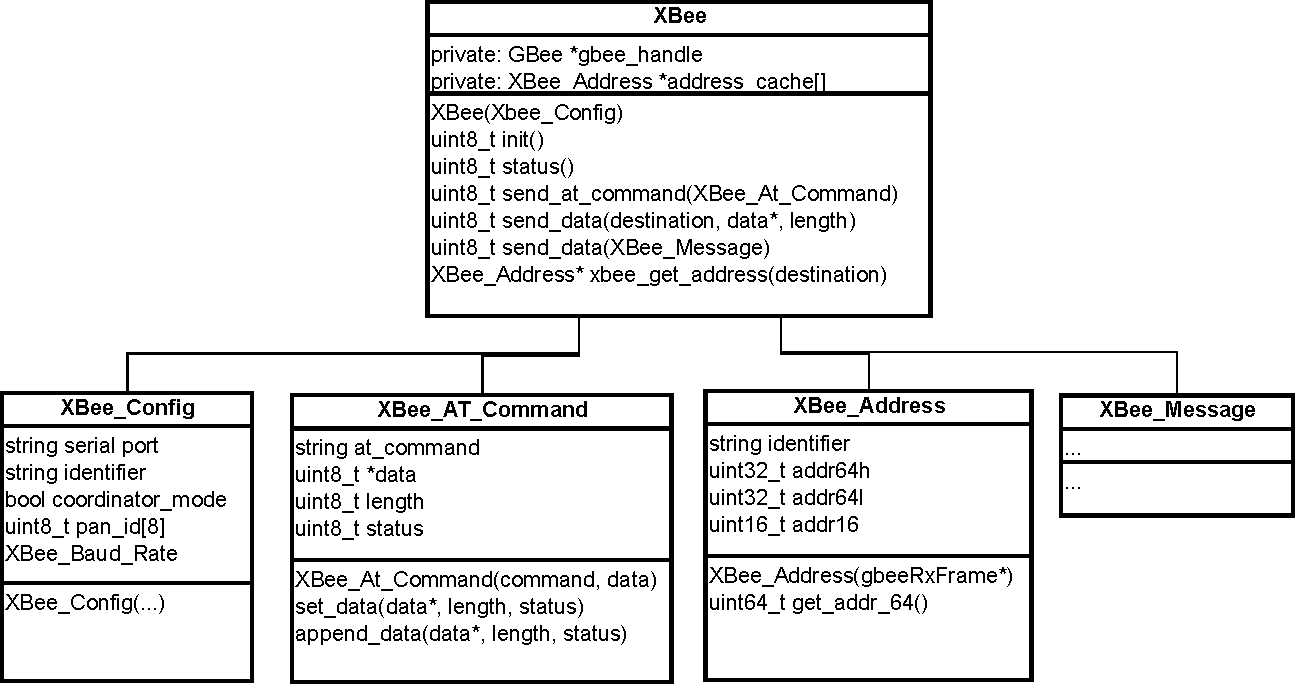
\includegraphics[width=\textwidth]{Images/xbee_interface}
\caption{Class diagram: XBee Interface}
\label{fig:xbee_interface}
\end{figure}

A C++ wrapper and a number of utility classes were developed to simplify data transmission and control of XBee devices (from the viewpoint of the core application). Figure \ref{fig:xbee_interface} shows the public interface functions of this wrapper and the utility classes will be discussed in the following sections

\subsection{Message handling}
The size of data frames that can be transmitted over ZigBee networks in one transmission is limited to a payload size of 84 Bytes. Our system needs to be capable of sending and receiving messages that exceed this size limit by multiple factors. For this purpose a XBee\_Message class was implemented that takes care of chopping arbitrary sized messages into frame sized pieces and re-assembling messages from received frames. 

\subsubsection{XBee\_Message}
\begin{figure}
\centering
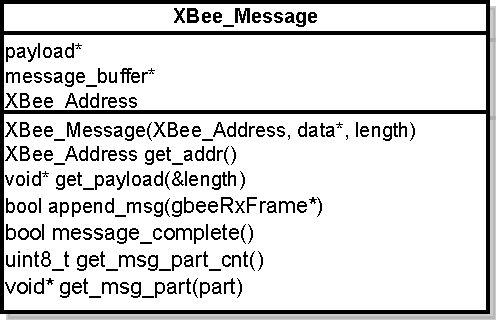
\includegraphics[width=0.5\textwidth]{Images/xbee_message}
\caption{Class diagram: XBee Message}
\label{fig:xbee_message}
\end{figure}

The XBee\_Message class expects a pointer to the data that should be packed into the message and the size of the data field. During instantiation the data is copied into a object internal buffer and the object takes over the responsibility for handling the allocated memory. 

The XBee interface uses objects of this class internally for message handling and also accepts objects of this kind as parameters for the send function. When data is received over the ZigBee network, the append\_msg function of this class is used to reconstruct the messages consisting of multiple parts before passing a handle to a complete message object to the user.

The XBee\_Message class is aimed at handling arbitrary data of arbitrary size and does neither know nor care about the type of data it contains. It treats all data in exactly the same way. The definition of the data that allows us to give a meaning to it is done independently.

\subsubsection{Message Types}
\label{sec:message_types}
The previous paragraph explained how the XBee\_Message class is used to transfer arbitrary data between network nodes. This paragraph deals with the way in which meaning is added to this data.

We use an inheritance based approach to define message types. Inheritance is particularly suited for this case as we can group messages into categories that have many common fields and only limited need for specialization.

\begin{figure}
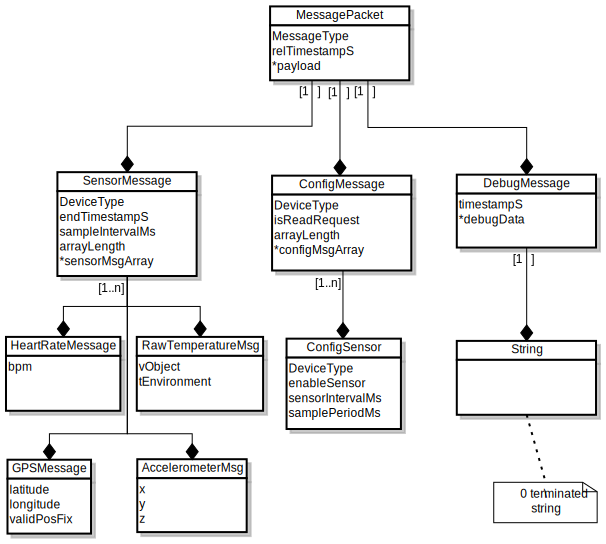
\includegraphics[width=\textwidth]{Images/message_types}
\caption{Class diagram: Message Types}
\label{fig:msg_types}
\end{figure}

This is implemented with structures instead of classes because structures guarantee that members are stored sequentially in memory which makes the job of serializing and de-serializing the messages for transmission purposes a lot easier.

The design of the message type classes allows to pack an array of multiple measurements (from the same sensor) into one message, which can help to increase the data throughput by improving to data to overhead ratio.

\subsubsection{Message de-/serialization}
\label{sec:message_serialization}
\begin{figure}
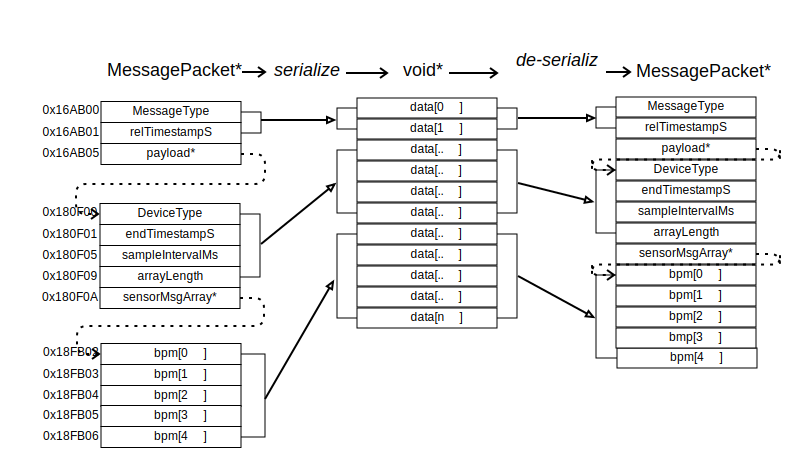
\includegraphics[width=\textwidth]{Images/msg_serialization}
\caption{Message serialization}
\label{fig:msg_serialization}
\end{figure}

The inheritance based message type data structures make extensive use of references, which is why they cannot be used for transmission as they are, but have to be serialized first. The process of serialization follows the references and copies all data of the message into a continuous memory area that can be transmitted across the ZigBee network, and deserialized into a message object on the other side. Figure \ref{fig:msg_serialization} depicts the steps involved in the process.

Message de-/serialization is implemented by two free-standing functions. The one that performs serialization expect a MessagePacket (see \ref{sec:message_types}) and a pointer to pre-allocated memory as arguments and copies the values from the MessagePacket into the continous memory. The deserialize function performs the inverse of this operation, and returns a MessagePacket that is an exact copy of the source MessagePacket, except for the destinations of the pointer members.

\subsubsection{Timestamps - relative and absolute timekeeping}
The timekeeping of the system is based on a the Unix style Real Time Clock (RTC), with the peculiarity that the monitoring devices do not count absolute time but time relative to the moment when they were first switched on. This decision is based on the fact that we cannot guarantee that the monitoring devices are able sync their internal RTC to the RTC of the base station when they are switched on (base station not in range, no GPS signal) which might lead to artifacts in the measurement data.

\begin{center}
\begin{math}
T_{abs} = RTC_{abs}- (T_{transmission} - T_{measurement})
\end{math}
\end{center}

To calculate the absolute time when a measurement was taken, the messages contain two relative timestamps - one that shows when the measurement was taken, and one that shows when the measurement was transmitted. The absolute time is calculated on the base station, right before the message is stored in the database.


\section{Base station software}
There are two independent software modules running on the base station software that use different Inter-process communication methods (IPC) to cooperate with each other. The receive and store module (R\&S) is responsible for the communication with the monitoring devices and storing received data into a database. The data presentation module on the other hand provides a graphical user interface (GUI) for the collected data and allows the user to configure the base station and the monitoring devices connected to the network.

The decision to divide the base station software into two independent parts was based on the fact that is is possible to create a very clear and well defined interface between the two modules. This allows us to develop the parts independently and use different programming languages that are best suited for the task. It also makes it possible to modify or replace the data presentation module without the need to adapt the rest of the system.

This is especially important in the case of the data presentation module, because we cannot foresee how the collected data is going to be used, and what is the optimal way of presenting the data to the user. In addition to that, the task of analysing and presenting the data was assigned to our sixth team member during the planning phase of the project, and had to be taken over by the rest of the team. For this reason we could not allocate as many man-hours to the presentation module as we would have liked, as it is a non-critical part of the system.

\subsection{Inter-process communication}
\subsubsection*{Database}
A file based sql database (sqlite3) is used to share the collected data and information about network status and node configuration between the two modules. The direction of communication is one-sided. The receive and store module writes to the database and when the user accesses the web interface the data presentation module extracts the requested information from the database. It can be seen as a passive way of communication as the one side who writes to the database does not care about the other side.


\subsubsection*{Message queues}
POSIX message queues are used to implement reactive communication between the processes, e.g. if the user requested a change of configuration in the web interface. The R\&S module will check the message queue periodically and react to them as promptly as possible. In case of messages that affect the base station the commands are executed almost immediately, in case of messages that concern monitoring devices, the messages are queued until the device connects to the base station, and the message can be dispatched.
\TODO{more details about mqueues?}

\subsection{Receive and store module}
The receive and store module sets up and controls the  ZigBee network and provides measurement data storage facilities in a sqlite3 database. It implements a simple state machine, waiting for incoming messages over the ZigBee network or the IPC message queue.

When there is incoming data from the ZigBee network, the module enters the receive state and tries to receive an XBee\_Message. When a complete XBee\_Message is successfully received, the message content is deserialized and stored into the database. When there’s not pending data left, the message queue is checked for messages destined for the node that just transmitted data. In case there are pending messages, they are dispatched, else the module goes back into the idle state.

When there is incoming data over the message queue, the module checks if the request can be handled locally in which case it is executed immediately. If the request is directed at a monitoring device, the R\&S has to defer dispatching the request until the next time the destined monitoring device connects to the base station. The reasons why the base station has to wait for the monitoring devices to open up a communication channel were explained in section
\ref{sec:wireless_connection}

\subsection{Data presentation module}
The data presentation module is written in Python and uses a lightweight Python web framework (flask\footnote{\url{http://flask.pocoo.org}}) to generate the web interface dynamically. 

The use of a dynamic programming language to generate the content that the user can see dynamically allows us to build a dynamic webinterface with a backend that’s communicating with the controller software. 

\subsubsection*{Web Interface}
The framework strictly divides display and logic parts of the website. The dynamic content of the pages is generated on the fly with the whole functionality of Python. This has the advantage that the menus of the website automatically get extended with sub-menus if a new monitoring device connects to the base station. 

\begin{figure}

\includegraphics[width=\textwidth]{Images/dummy}
\caption{Web Interface}
\label{fig:web_interface}
\end{figure}

The sensor data is currently displayed in dynamically generated static html tables. This allows a good quick overview over the collected data, but is suboptimal to analyze the data in more detail. In future versions this could be improved by using Ajax to display the tables, to offer better access to the collected data.










\chapter{PCB design}
In order to make a complete system and test it on adequate subjects without any harm to the circuitry it was decided to make a custom PCB and encapsulate it in a splash proof casing. PCB not only eliminates the accidental connection losses between the components as it usually happens on breadboards and protoboards but also keeps the traces short and ensures the components function according to their specification.
 
The schematic and layout were designed using CadSoft Eagle software version 6.1.0. It is not considered to be the most user friendly software in terms of the usage interface, but is fairly simple and straightforward. Furthermore, the user community is very large, therefore it is possible to find various component footprints already made by others to be used in the design. This decreases the overall time required to make a PCB design. Nevertheless, as we were using very specific components  (ANT, GPS, etc.) a footprint for them had to be designed manually by consulting the datasheet. 


\section{Schematic}
This section will describe the connections between different components of the system, their intended use and operational principles. Full schematic of the system can be seen in section \ref{sec:pcb_schematics} of the Appendix. It is separated into different sheets for ease of reading.
 
\begin{figure}
\centering

\includegraphics[width=0.8\textwidth]{Images/dummy}
\caption{Block Diagram: Parts}
\label{fig:block_parts}
\end{figure}

\subsection{Power conditioning}
This part is responsible for providing energy to the rest of the board. The circuitry consists of two stages, see \TODO{Appendix\_Power\_LDO.pdf} First stage incorporates a constant current constant voltage single cell Lithium Ion battery charger centered around a ADP2291 chip from Analog Devices. The second stage is a low dropout voltage (LDO) regulator based on a ADP1706 chip from the same manufacturer.



\subsubsection{Battery charger}
The input voltage of the charger is in the range of 4.5 to 12V, therefore no power supply providing higher voltage than this is allowed to be used. D1 acts a reverse voltage protection diode in case the power supply is connected with a reversed polarity to the board. In case this ever happens it will not cause any damage to the components. 


C4 and C16 capacitors are used to filter out the noise that might come from the power supply. The chosen values of 820uf and 0.68uf are sufficient for this purpose. Resistors R2 and R6 placed in series with a battery provide current measurements for the charger. Hence, the charging current is adjusted by changing the R2 and R6 resistor values, that is currently set to 750mA. Internal LED driver is used to indicate the charging status of the battery. Charge status LED1 is ON when the battery is charging. Transistor Q1 acts as a pass device which provides a charging current to the battery. It was chosen with a reserve in parameter specifications. The device can handle continuous collector current of 3A and has a $V_{ceo}$ of 60V. This enables the device to function properly not only in the current setup but in a scenario when a higher current is required for faster charging. As a driver requirement the transistor has to have a certain minimum PNP beta (hfe coefficient), which for current configuration has to be no less than $I_{max} / 40mA $, where 40 mA is the base drive current and Imax is the charging current. This gives us the minimum beta of 18.75 that the transistor has to have. The chosen one has an hfe of 80 at collector current equal to 1A. 

In order to keep it from overheating a thermal protection is used by utilizing the NTC1 thermistor. This enables the charger to monitor the temperature of a pass device and decrease the charging current accordingly. Shutdown temperature of the charger is set internally to 100C. 

The charger works in step-by-step sequence illustrated by diagram \ref{fig:charger_sequence}:

\begin{figure}
\centering

\includegraphics[width=0.8\textwidth]{Images/dummy}
\caption{Battery charging sequence}
\label{fig:charger_sequence}
\end{figure}

\begin{itemize}
\item \textbf{Power-down:} If the input voltage is lower than 3.8V the charger is in the shut-down mode. Power consumption from the battery is $1\mu A A$.
\item \textbf{Pre-charge:} When a voltage higher than 3.8V is detected at the input of the charger the charger checks the voltage across the battery and enters a pre-charge state if the battery voltage is lower than 2.8V. In this stage the maximum supplied current is 75mA. In cases where battery is deeply discharged and measures less that 1.5V the supply current is set to 150mA. 
\item \textbf{Fast charge:} If the voltage is higher than 2.8V the charger enters a full current fast charge mode which continues until the battery voltage reaches 4.1V 
\item \textbf{End-of-charge:} The charging current is reduced as the battery reaches its full capacity and once this current is less than 75mA an end-of-charge mode is initialized. 
\item \textbf{Shut-down:} This mode will be initialized if the voltage on pin Vadjust drops down below 0.4V.
\end{itemize}

Capacitor C6 determines the time of all operation modes. The ratio between the fast charge mode to pre-charge and end-of-charge is always 1/6. Given the capacity of our battery is 2200 mAh time required for it to fully charge with current settings is 2.9 hours. Therefore a timeout of 3 hours for fast charge mode is sufficient. C6 capacitance is calculated from the following formula $Ct = tchg *  1uf / 1800$ and is equal to 0.1 uf. The pre-charge and end-of-charge modes timeout in 30 minutes. Time limit of the fast charge mode is required as a precaution in case the battery fails to reach end-of-state mode for any reason.


\subsubsection{LDO regulator}
The LDO regulator takes in the provided voltage by the battery and outputs a fixed value of 3.3V required to power all on-board devices. Decision to use this type of regulator was made from the fact that the difference between input and output voltage is very small. Therefore, using a traditional linear regulator in this case is not an option. Our chosen device has a maximum dropout voltage of 55mV at 100mA output current. This figure increases to 345mV at output current of 1A respectively. The latter dropout will never be achieved, as in the worst case scenario when all peripherals are operational the maximum current consumption will be \TODO{check:} datasheet GPS, ANT, Xbee SD card + MCU 9.6mA
 all peripherals combined will hardly ever pass the 100mA current consumption point.
 
This LDO regulator was designed for operation with small value ceramic capacitors for space saving applications. Nevertheless, using a larger value output capacitors improves the transient response. Hence, as space is not an issue a value of 150uF was chosen. The regulator has a built in accidental short circuit protection. If for any reason the output becomes shorted, the regulator will conduct the maximum amount of 1.5A current into the short, increasing the junction temperature to critical level and triggering the thermal protection as a result turning off the output. 

A soft start function is implemented by connecting the C3 capacitor to ADJ pin of the regulator. This ensures a gradual output voltage ramp-up. The ramp up time is calculated using the following formula $T_{ramp-up} = 0.8V × (C3/1.2uA)$ Tramp-up represents the time it takes for the output to reach 90\% from 0\%. In current configuration where the value of C3 is 10nf the ramp-up time is 6.67 ms.

To insure a stable power supply to all components organic solid capacitors with conductive polymer (OS-CON) are used. Their benefits are discussed in 
\href{http://www.capacitorlab.com/capacitor-types-polymer/}{capacitorlab}  and  \href{http://www.capacitorsplus.com/whatis.htm}{capacitorplus}


\subsection{MCU}
As was mentioned earlier the MCU used for the project is EFM32GG332 based on ARM Cortex M3 core with a 1024KB of Flash and capable of running at a 48MHz speed. The chip has several clock sources and different crystal oscillators are used to generate that clock. XT1 is a high speed oscillator (HFXTAL) rated at 48MHz and running in a fundamental mode \TODO{}see Appendix\_MCU\_decoupl\_osc\_reset.pdf. 

XT2 is a low frequency oscillator (LFXTAL) rated at 32.768KHz and is produced by MEMS processing technology. This oscillator is used for peripherals running in low energy modes and operates in fundamental mode as well. The MCU will not work with a high speed oscillator that is specified to operate in an overtone mode. To insure that the crystal operates correctly, it has to have a certain load capacitance, in our case for XT1 this is 18pF and for XT2 it is 7pF. 

In case there is a need to reset the MCU it can be done by using the S1 global reset button. Capacitor C14 is used in parallel with the switch to implement a hardware de-bounce function. 

A standard approach for decoupling is used. One large capacitor C2 rated at 150uF is used for the whole system with 0.1uF C7-C12 capacitors used to decouple separate power pins. In our design we are not using ADC of the MCU; therefore it was not necessary to separate the digital and analog power domains. Separation is usually done to ensure better isolation and noise suppression between the power domains.


For programming and debugging the custom made PCB a debug interface consisting of clock input (SWCLK), data in/out lines (SWDIO) and serial wire output (SWO) had to be exposed, see \TODO{}see Appendix\_Debug\_Mic.pdf. An external development kit was used to program/debug the PCB. By supplying the power to the PCB from the development kit via VMCU pin it was possible to measure the current consumption of a target with an Energy Aware profiler.


\subsection{I2C devices}
The TMP006 MEMS sensor from Texas Instruments was chosen for its ability to measure the temperature without the need of making a contact with an object. The measurement is done by allowing the thermopile to absorb the IR energy emitted from an object and based on the thermopiles voltage change determine its temperature.

Temperature sensor uses SMBus for transmitting transmit the data. The address of the device on a bus is set to 1000000 by grounding ADR0 and ADR1 pins. DRDY pin indicates whether the data is available to be read by the MCU and requires a pull-up resistor in order to operate correctly. Decoupling of the sensor is performed using a 22uF OS-CON and a 0.68uF plastic film capacitors.

The I2C bus is shared with an accelerometer. As this is not the only mode the accelerometer can operate the I2C mode had to be set by pulling the CS pin high. By setting the SDO/ ALT ADDRESS pin to high the accelerometers address becomes 0x1D on the bus. No pins are left floating in order to prevent leakage currents. Hence the Reserved\_3 pin is connected to +3.3V and Reserved\_2 together with Reserved\_1 are grounded. Optionally they can be left floating. 
The device can operate in several power supply modes. In this particular design it operates in a single supply mode, where VS is connected together with VDD/IO. Decoupling is performed for both of the pins using two 0.1uF ceramic capacitors. In addition to that a 22uF OS-CON is used at the VS pin to minimise the digital clocking noise.

\subsection{RF devices}
Despite the fact that Xbee has a lot of pins, the only connections that are required for it to be operational are VCC, GND, DOUT and DIN. Others are not used in this case. Xbee is connected to USART 0 of the MCU as it requires high baud rate communication.

The GPS module on the other hand is connected to low energy UART (LEU0). By default its communication rate is set to 9600 baud. The GPS module requires two power supplies. VCC is the first one and is used for digital parts together with I/O. VBAT is the second one and is used for non-volatile back-up block. By default GPS does not have low energy mode that can be switched on demand, it does go into low energy mode automatically once it has acquired the satellite positions and collected the Almanac data. In normal operation mode GPS typically consumes 115mW of power which translates to 35mA of current draw from the battery. Nevertheless, this figure can rise up to 40mA. Power consumption drops to 75mW (22mA current draw from battery) once the GPS has finished with the cold start. This figure is still high. Power supply can be switched off for the VDD block if the navigation is not needed. This will enforce the GPS to enter the backup mode. The power then will be drawn from VBAT which is used for keep the collected satellite data in RAM. This will ensure a fast TTFF (time to first fix) once power on VDD is re-applied again. Power draw in this mode is in the region of 15uW (4.54uA).
The PPS (pulse-per-second) output is not used in the design as it is only required for timing purposes. For decoupling purposes a 0.1uF ceramic capacitors are used for both power pins with an addition of 22uF OS-CON for the VCC.

ANT module is connected to low energy UART 1 (LEU1). Baud rate selection is made by setting the dedicated BR1-BR3 pins either low or high. In the system the pins are pulled down which gives us the speed of 4800 baud. 

When not in use Xbee, GPS and ANT modules can be completely shut off to save more energy. This is done by means of P-channel mosfet. N-channel mosfet is not acceptable in this case, because the devices are ground referenced. By default these modules are ON and setting the correct mosfet high will shut-off the power to the device. Shutting down both power supplies for the GPS will trigger the loss of all stored satellite data in the non-volatile block. Therefore, once the GPS becomes operational it will have to go through the cold start again and use a lot of energy.

\subsection{Microphone}
MEMS microphone is connected to the USART1 of the MCU. There is a possibility of using two microphones in a stereo configuration. Nevertheless, in this design only one channel was used. The L/R pin that is responsible for channel selection was grounded indicating that Left channel is used only. SD pin requires an external pull-up resistor. To our advantage MCU has an integrated one, therefore this one was used instead of an external one.


\section{Layout}
The PCB layout was made not only for the final board, but for several breakout boards as well. The accelerometer and MEMS microphone both have a specific pad. Therefore, the breakout boards were custom made for them. This enabled us to speedup the prototyping process and use these devices prior to the assembled PCB. The accelerometer breakout board is not used for the final product, but the microphone board is as it is mounted to the head of a stethoscope. PCB layout for the microphone can be seen in Appendix \ref{fig:pcb_layout_mic}. The layout of the final board is shown in  Appendix \ref{fig:pcb_layout_bottom} and Appendix \ref{fig:pcb_layout_top}. It is a 2-layer board, therefore a layout for both top and bottom is provided.
The final component placement can be seen in figure \ref{fig:board_layout}. 

\begin{figure}[!htb]
\centering
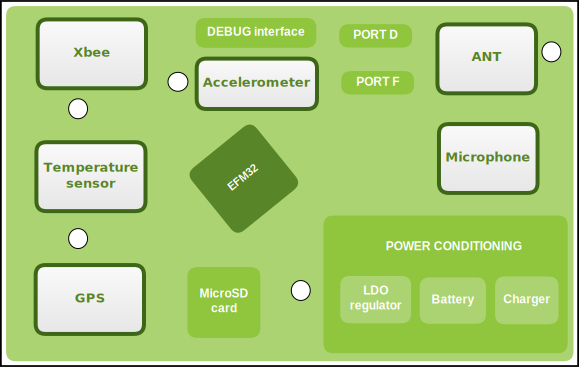
\includegraphics[width=\textwidth]{Images/board_layout}
\caption{Main component placement on a PCB}
\label{fig:board_layout}
\end{figure}

When positioning the components on the PCB some considerations had to taken into account. These are going to be discussed step by step starting with the power conditioning circuitry. 

The pass transistor Q1 used in the Charger generates a lot of heat, according to the calculation:
\begin{flalign}
P_{Diss}(W) = I_{MAX} x (V_{ADAPTER(MAX)} - V_{PROTECT} - V_{RS} - V_{BAT}) 
\end{flalign}

When 750mA of current ($I_{MAX}$) is flowing through it and the input voltage (VADAPTER(MAX)) can take the maximum value of 9V Q1 dissipates 4.38W of power. In order to keep a low profile board the PCB itself acts as a heatsink. The pad of the transistor that draws away the heat from the crystal cannot be connected to the largest copper area of the board - GND, as the pad is internally connected to Vdd. Therefore a dedicated area was left for that purpose and thermally isolated from the neighbouring components. 

This also prevents the shortening of their lifespan. Multiple vias are used to connect the upper layer of copper with the bottom one making the heat dissipation more efficient. In case of overheating the NTC1 should tell the charger to decrease the current passing through the transistor lowering the power dissipation. Hence, the NTC1 was placed as close as possible to the transistor and was surrounded by the copper heatsink.


The LDO regulator has a SOIC package with an exposed pad underneath it. This is done to dissipate the generated heat directly into the board. The pad is internally connected to GND and in this case it was unnecessary to make dedicated heatsink area for this chip. As with the Multiple vias connect the upper and bottom layers of the PCB to promote better heat transfer.

The LDO regulator has a SOIC package with an exposed pad underneath it. This is done to dissipate the generated heat directly into the board. The pad is internally connected to GND and in this case it was unnecessary to make dedicated heatsink area for this chip. As with the previous heatsink design multiple vias connect the upper and bottom layers of the PCB to promote better heat transfer.

TMP006 temperature sensor used in the project is one of the kind and has to have a specific board layout in order to function correctly. The TMP006 is affected by the IR energy from below the sensor as it is affected by the IR energy coming from objects that are in its field of view. In case the temperature of the sensor is the same as the PCB there will be no energy transfer between them and the sensor will function without errors. Nevertheless, if there is a difference between the PCB temperature and the die temperature it will cause the heat energy to be conducted through the thin layer of air and this will introduce offset to the voltage readings making the temperature calculations incorrect.  In order to avoid this several factors had to be addressed:

\begin{itemize}
\item Thermal time constant matching of the PCB to the temperature sensor
\item Thermal isolation of the TMP006 from any heat sources
\end{itemize}

Difference in thermal time constants can generate temperature mismatches between the PCB and TMP006 die until the temperatures stabilize. In order to avoid this and bring the constants close to each other a small copper fill under the temperature sensor is placed and connected to GND (see figure \ref{fig:constant_matching}). An island of copper surrounds the the sensor and helps with the constant matching as well. Without the copper fill the temperature between the sensor and PCB will never achieve equilibrium, unless the system was in equilibrium for an extended period already. 

\begin{figure}
\centering

\includegraphics[width=0.5\textwidth]{Images/dummy}
\caption{Constant matching}
\label{fig:constant_matching}
\end{figure}

The second factor addresses the thermal isolation problem. The sensor has to be isolated from devices that act as a heat source, this includes any active component placed near it. When the device becomes operational it dissipates a certain amount of heat into the ground plane, this in turn raises the temperature of the TMP006 as GND is common and could cause the same problems as with the thermal time constant mismatch. To address this issue the sensor and the copper island was isolated by low k material (see figure \ref{fig:thermal_barrier}. In this case the PCB material is used as an insulator.

\begin{figure}
\centering

\includegraphics[width=0.7\textwidth]{Images/dummy}
\caption{Thermal barrier}
\label{fig:thermal_barrier}
\end{figure}

This isolation prevents the unwanted thermal interaction with other devices. Moving the device away from any source of heat would be the best solution. This way any drastic temperature changes would be invisible the temperature sensor.

Accelerometer has a mechanical issue that has to be addressed. In order to prevent any PCB vibrations being visible to the accelerometer it had to be mounted close to the PCB hard mounting point. 

Several modules have integrated antennas in them, these are ANT, Xbee and GPS. No special PCB placement is required for them other than taking mechanical considerations into account. Any device containing metal should be kept away from the field of view of the integrated antenna to avoid signal scattering and reflections. Otherwise this could lead to an effective loss of signal radiation resulting in the reduction of the transmission range. Hence, modules were placed on the edges of the PCB and the GND plane was removed from the antennas field of view. 

\begin{figure}
\centering

\includegraphics[width=0.5\textwidth]{Images/dummy}
\caption{Measured voltage noise}
\label{fig:voltage_noise}
\end{figure}

The most practical way of placing the MCU is to put it in the center of the PCB. This enables the usage of short trace connections to the peripherals located on the sides of the board. Decoupling capacitors are placed as close to the component power pins as possible. This applies to all ICs and modules used on the board without any exceptions. By doing this the voltage noise can be dropped to a very low figure. In the system the measured noise was 4mV, as it can be seen in figure \ref{fig:voltage_noise}

Oscillators are placed as close to the MCU as possible to avoid any additional trace capacitance and delay, which would change the generated frequency. 

Taking all these considerations in mind the board was routed manually as this ensures the correct placement of the tracks and special zones needed for components. A good layout will always result in a proper functionality of the PCB and will reduce the probability of redesign.


\subsection{Soldering}
Soldering of components was done using several tools. This included a hot plate for reflow process and conventional tools for SMD components. Temperature sensor and an accelerometer were attached to the PCB using solder reflow as it was impossible to do solder them using conventional tools. An appropriate thermal profile had to be followed to prevent damage to the components. Both ICs have a peak soldering temperature of 260C but a slightly different thermal profiles, figure \ref{fig:temp_profile_optimal}(a) and figure  \ref{fig:temp_profile_optimal}(b) show the thermal profiles for temperature sensor and accelerometer respectively. 

\begin{figure}
\centering
\mbox{
\subfigure[]{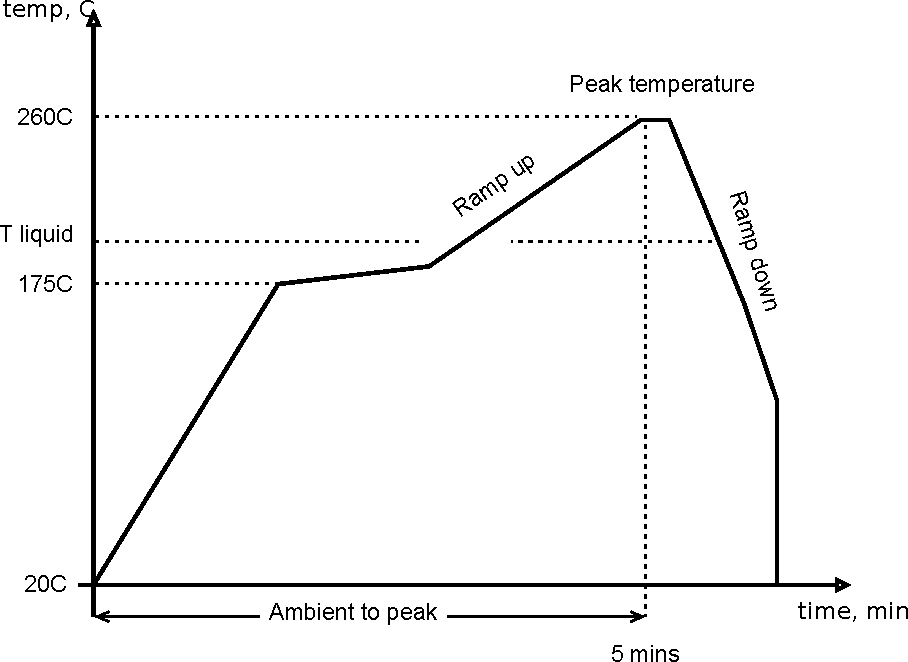
\includegraphics[width=0.45\textwidth]{Images/Thermal_profile_for_TMP006}}\quad
\subfigure[]{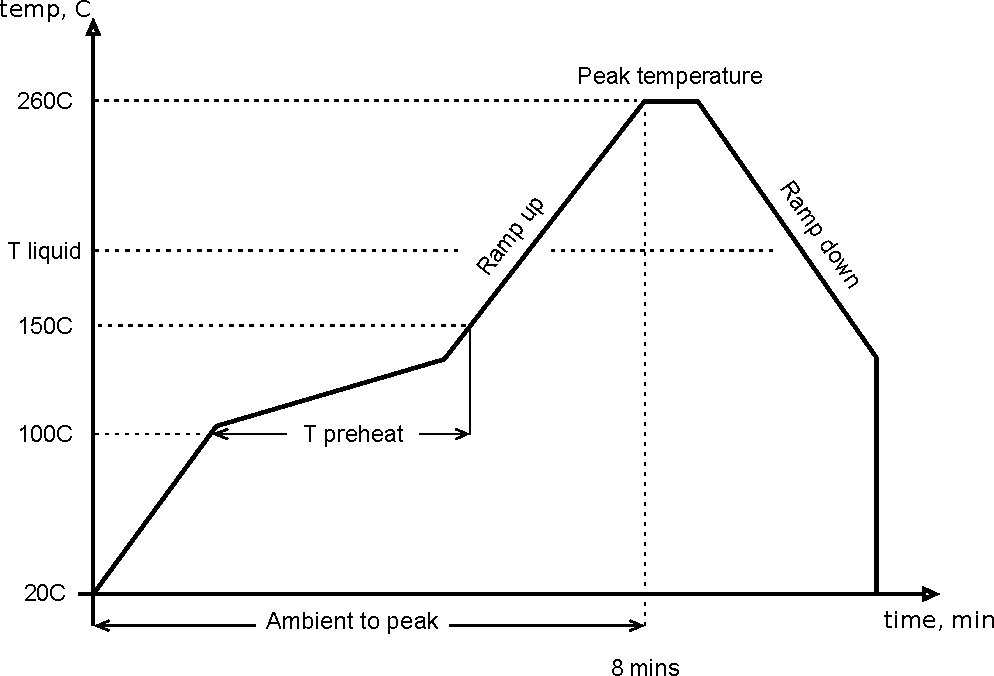
\includegraphics[width=0.45\textwidth]{Images/Thermal_profile_for_ADXL350}}
}
\caption{Optimal temperature profiles for soldering}
\label{fig:temp_profile_optimal}
\end{figure}

Ideally It should take no longer than 7 minutes to achieve the peak point from ambient temperature. This way the BGA package balls of temperature sensor would melt and produce a reliable contact to the PCB traces and accelerometer  without any risk of damaging the device. Nevertheless, the suggested profile for both ICs was impossible to achieve with the used hot plate as it only had an option of setting the end temperature point which took considerable time to reach. On average this time was 13 minutes as seen from the plotted thermal profile provided by the hot plate, figure \ref{fig:temp_profile_used}.

\begin{figure}
\centering
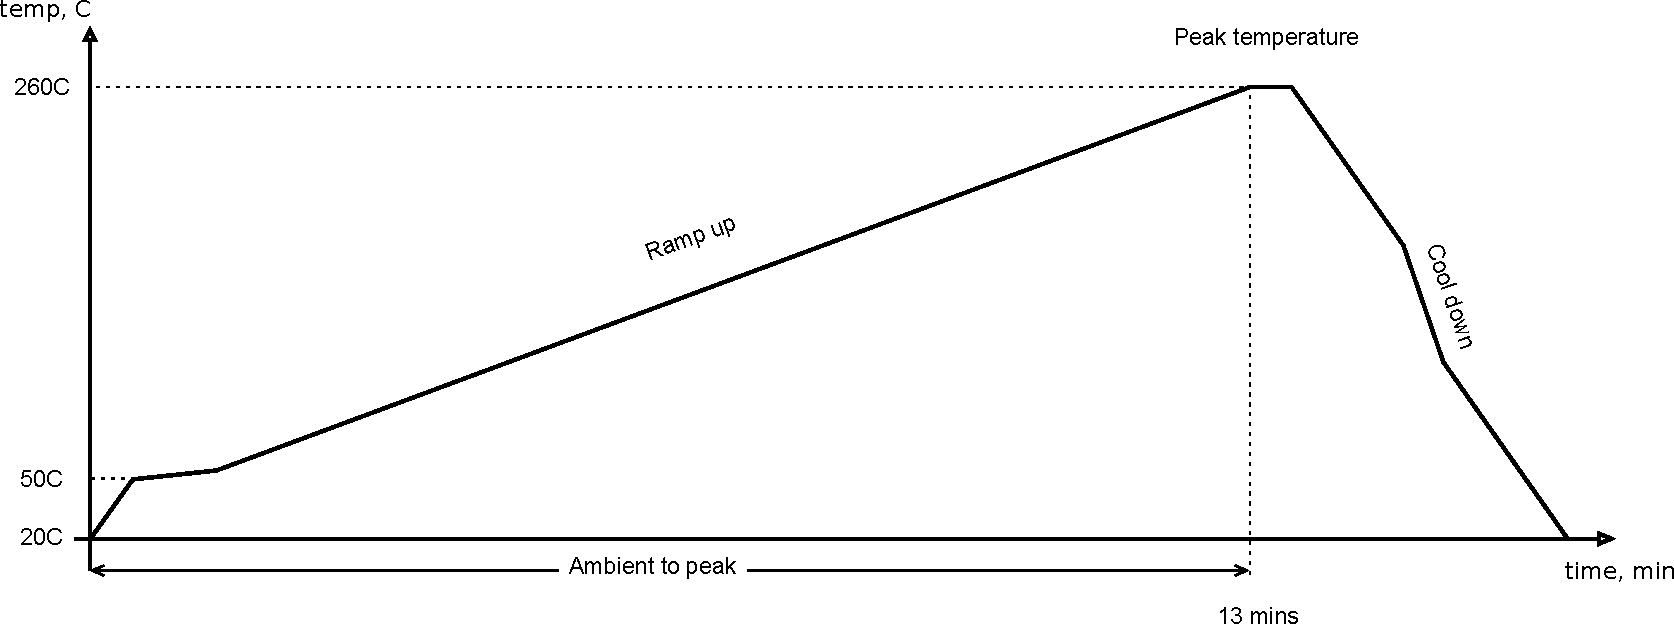
\includegraphics[width=\textwidth]{Images/Thermal_profile_used}
\caption{Used temperature profile for soldering}
\label{fig:temp_profile_used}
\end{figure}

It did increase the risk of damaging both of the components. Nevertheless, after the reflow they functioned as expected.


\section{Case design}
Several options for the case have been considered, including the usage of rapid prototyping facilities to make a custom case to fit the PCB. Due to high cost of the material used in production and limitations set on our budget it was decided to exclude this option. Case for the PCB was ordered through Maplin online store and rapid prototyping facilities were used to make a custom part that would attach the MEMS microphone board to the head of a stethoscope instead. Case is made of plastic, which is not the best solution, considering the horse might damage it while rolling around. The optimal solution would be to use a metal case, this would prevent it from being damaged in the harsh exploitation environment. Nevertheless, this is not an option, as metal would act as a shield for RF signals either completely blocking them or diminishing to an unacceptable level. 

\begin{figure}
\centering

\includegraphics[width=0.4\textwidth]{Images/dummy}
\caption{Exposed System in a case}
\label{fig:case_monitor}
\end{figure}

The head of the stethoscope was then integrated into the case and isolated to ensure a decent level of splash proofness, as depicted in figure \ref{fig:case_monitor}.

The Complete encapsulated system is shown in figure \ref{fig:complete_monitor}. The stethoscope head protrudes slightly from the case enabling a better contact with the horse under test. The case is certified to be splash proof according to IP54. This way the PCB might be protected even in rainy weather. 

\begin{figure}
\centering

\includegraphics[width=0.4\textwidth]{Images/dummy}
\caption{Completed encapsulated system}
\label{fig:complete_monitor}
\end{figure}
\chapter{Testing}
In order to verify the correct behavior of our system, independent unit tests of each each subsystem were performed, before integrating them into the rest of the system. The verification of the test results was done manually and not by using a set of autonomous testbenches, as the test-driven methodology is still new and uncommon in the field of embedded systems.

\section{Wireless communication}
\label{sec:wireless_testing}
The functionality of our system depends on a wireless connection, which is why we needed to ensure that we can guarantee a stable connection and reliable transmission of data over the wireless link, while being able to transmit data at a reasonable data rate.

To verify that the connection fulfils these requirements we ran a stress test, where two devices, one configured as network coordinator, the other configured as a network node, exchanged small data packets over a long period of time (>4h). 

The reliability of the transmitted data was tested by sending a predictable set of values between the network nodes and aborting the test when receiving a value that differs from the expected value. 

The stability of the connection was tested by imposing a timeout limit on both sides of the connection. If no data was received within a defined timeframe or no acknowledgement was received the test was also aborted.

When the system passed this stress test and we could rely on a stable and reliable connection we had to verify the last of the three requirements - the data throughput.

To test the data throughput we used the XBee interface we had developed to transmit messages larger than the maximal ZigBee frame size. The throughput was obtained by sending a defined amount of data and measuring the delay between sending and receiving the acknowledgment for the last part of the message. The results can be seen in figure \ref{fig:xbee_throughput}.

\begin{figure}
\centering

\includegraphics[width=0.8\textwidth]{Images/dummy}
\caption{XBee throughput}
\label{fig:xbee_throughput}
\end{figure}

The throughput test revealed that the chosen wireless protocol is not able to transmit data nearly as fast as we expected. The maximal throughput that can be reached by our system is 13kbits/s, which is about 20 times slower than what we had expected (ZigBee data rate is often quoted as  250kbit/s). 

It turned out that the firmware for the devices we are using (XBee) imposes a large additional overhead on the protocol and that even using a pure ZigBee implementation the data rate of 250kbit/s can never be reached, because the ZigBee standard itself uses part of the data rate to implement its functionality and vendor specific ZigBee implementations add even more overhead. The XBee device manual states this in a subsection, that we didn’t take into account during the design phase. The maximal data rate that is specified for network using our configuration is 16kbit/s.

This result has a strong influence on our system, because it renders wireless transmission of audio data infeasible. A small calculation shows why

\begin{flalign}
t_{transmission} &= \frac{data rate*t_{duration}}{f_{transmission}} \\
& = \frac{128kbit/s*240s}{13kbit/s} \\
& = 39min
\end{flalign}

It takes 39 minutes to transmit a 4 minute gut sound recording, which conflicts with our goal of a battery powered energy efficient system, because the processor has to be awake while transmitting the data over ZigBee and the battery runtime would decrease drastically.

The current solution for this problem, is to store audio recording on a removable SD card in the monitoring device. Proper solutions for this problem are discussed in the Future Work Chapter (\ref{chap:future_work})

\section{Field Testing}
Throughout the development process, the team did not have access to a horse and there is almost no sample gut sound recordings available online. After the integration and PCB production phases were complete, the whole system \TODO{} was tested on human subjects since the subsystems of the monitoring device are usable on humans as well. The only horse-specific part of the system was the gut sound monitor - although it is also usable on humans, the design was not made with humans or species other than horses in mind. 

In the laboratory environment, the team could only test the gut sound monitor on human subjects to record heart beats since human gut sounds are not as periodic and loud as those of a horse. Human heart beat recordings were made without problems, and four beats of an approximately 65 BPM heartbeat with the S\_1 and S\_2 (respectively the "lub" and "dub" sounds) can be clearly seen in figure \ref{fig:heartbeat}

\begin{figure}
\centering
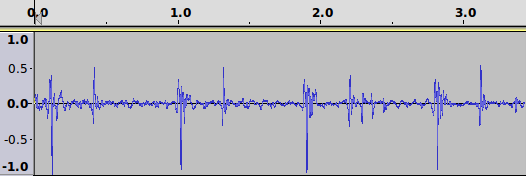
\includegraphics[width=0.8\textwidth]{Images/heartbeat.png}
\caption{Testing results: heartbeat}
\label{fig:heartbeat}
\end{figure}

However, this is not the real usage of the module. Thus, the team made a field trip to New Forest to perform gut sound monitor testing on equines. Gut sounds of three horses were recorded from different sites of the abdomen. Each recording was done one minute long and saved in the SD card. The result was satisfactory although the environment was noisy because of the horses' movements and conversations. Therefore, noise cancellation filter is needed to improve the performance. The recordings can be found in the Appendix \ref{sec:recording}.

\begin{itemize}
\item no gut sound recording was available on web
\item we could test the integrated system (temperature etc on humans) but gut sound is horse-specific so we arranged a field trip. (TODO{} not sure if we should add thıs ınfo: + testing the whole components on gut requires more time, components and people) and it was not crucial, because complete system testing was successful.
\item we did gut sound recording on 3 horses from different parts of the abdomen, each 1 minute long. although the environment was noisy (horse was moving, conversations etc) the recordings were successful. They can be found in appendix. A noise filtering needed to get better results.
\end{itemize}



\chapter{Results}
\TODO{}
\chapter{Project Management}

\section{Development Phases}
To accomplish the objectives in the limited timeframe, development was planned in a way that would allow maximum parallelization of developer resources and tolerate unforeseen delays by leaving some unallocated time at the end. The development consisted of the following main stages:

\begin{description}
\item{\bfseries 1. Project planning and system design:}
The first step was to define the scope of the project, identify the main tasks and come up with a Gantt chart to schedule the tasks. Since 	the project was assigned to the team in the second week of the semester, the team had to start working on the project later than the official start date, which resulted in a tighter schedule. The top-level system design was also completed in this stage. The  approach to design a distributed system with multiple energy-efficient wireless monitors and a base station was accepted. Functional requirements from the hardware were also determined according to the given specification.

\item{\bfseries 2. Background research:}
The team researched the existing solutions for equine health monitoring, identified the applications of the resulting system and familiarized themselves with energy efficient implementation methods. As stated in section \ref{sec:research_discussion}, discussions with field experts resulted in narrowing the scope of the implementation to a data collection tool for general monitoring and research since diagnosis of grass sickness was not considered feasible with our approach.

\item{\bfseries 3. Component research and ordering:}
This stage consisted of searching for the hardware components that fulfilled the requirements identified in the previous stage. Decisions were made on the basis of energy efficiency, ease of development and stock availability of each component. Some components had to be ordered from non-ECS suppliers as they were not available from school suppliers. There were some delays in ordering and receiving the components which had a negative impact on the schedule because they prevented the team from starting with the next phase and pushed the work on hardware-dependent tasks in the system further back into the schedule.

\item{\bfseries 4. Hardware subsystem prototyping:}
In this stage the team members worked in parallel on getting each hardware subsystem functional, writing drivers for them as described in chapter \ref{chap:hardware_subsystems} and making the implementations energy efficient and stable. 

\item{\bfseries 5. Integrating subsystems, system software:}
This stage involved connecting together the implemented hardware subsystems into a single functional system, and creating the 	software frameworks on both the monitoring device and the base station to implement the desired data flow. A completely integrated prototype of the monitoring station on a development board allowed the team to test and verify the distributed nature of the system architecture before the custom PCB was ready.

\item{\bfseries 6. PCB design, production and case:}
Ran in parallel with the other tasks, this stage involved designing the final printed circuit board (PCB) that would later be placed inside a stable case and became the core of the monitoring device. The experience gained during the hardware subsystem prototyping stage was infused into the PCB design process, which meant that the design of each sub-module on the PCB was tested and verified before the final PCB was ordered. 

\item{\bfseries 7. Testing the integrated system:}
Once the integration and PCB production stages were complete, the system was integrated on the PCB and tested with separate unit tests for each hardware subsystem.  Due to careful individual prototyping and the previous successful integration on the development board of a complete prototype the final stage went relatively smooth and did not cause any delays in the schedule. The resulting completed prototype was also tested on human and horse subjects.
\end{description}

The time slots allocated for each task can be found in section \ref{sec:gantt_chart}

Within the given timeframe the team managed to design and build a working prototype of the distributed system, which was almost feature complete according to the specifications. Please consult the chapter \ref{chap:results} for details.

\section{Resources}
\subsection{Hardware Development Tools}
he core of the monitoring device system is based on an Energy Micro microcontroller. Because some of the team members had worked with Energy Micro devices in the past we had access to three Energy Micro starter kits (STK), and were supported by Energy Micro who supplied us with an additional starter kit\footnote{The team joined the \href{ http://forum.energymicro.com/forum/49-efm32-design-contest-2012/}{Energy Micro EFM32 Design Contest 2012}  with this project and qualified as one of the best design ideas. One of the starter kits was received as an award from this competition. The team will also compete at the final stage of the contest with the final product.}
and a development kit (DVK). 

Having access to four STKs enabled us to build build the subsystems in parallel on a very similar hardware platform that is also used for the final product. The more powerful DVK was used to integrate them before the custom PCB arrived. The custom PCB layout had to be sent for manufacturing as there are no facilities to produce the board in-house. Typical turnaround can be up to 7 days. Nevertheless, this is a very crucial component to the project and delay would result in significant setbacks. Hence, it had to be ordered with a faster turnaround.

PCB assembly was done in the GDP lab using the following conventional tools: soldering and hot air stations, microscope, tweezers, etc. Hot plate was used for solder reflow of wafer chip scale components. Breadboards and wires were provided from the start of the project and aided in the prototyping stage. Oscilloscopes and multimeters were used for testing and fine-tuning the PCB modules.


\subsection{Team}
The development team initially consisted of 6 people. However one member, Ahsan Baig, had to drop the project after the sixth week since he could not enter the UK due to visa issues.

The initial project planning was made considering six project members. As it was unclear from the beginning if Ahsan would manage to arrive in time for the project, he was mostly assigned tasks that were extensions for the overall system and could be integrated in the later stages of the project, such as display and analysis of collected sensor data. After it became certain he would not be working with the team his tasks were distributed among the rest of the team or, as in the case of data analysis, discarded. 


\subsection{Research}
To gain a deeper insight into the physiology of horses and horse related health issues, contact was established with experts in the field: Dr. John Chad, lecturer at Biological Sciences and Dr. Neil Smyth, lecturer at Development and Cell Biology, both from the University of Southampton.

The initial contact led to a meeting where Dr. Neil Smyth took the time to give an enlightening presentation about the digestive system of horses.

The discussion after the presentation helped us to have a more realistic view on the goals of our project and excluding data analysis and diagnosis from the project scope, because even expert veterinarians have difficulties diagnosing grass sickness disease. A discussion of the reasons for this decision are provided in the chapter \ref{chap:research}.



\section{Task Distribution}
Project tasks were distributed considering skills and interests of all group members. A high degree of parallelisation of tasks was needed to comply with the tight schedule. A shared Google document was used to record the tasks and their status, which can be found in section \ref{sec:task_breakdown}. All members attended discussions about system design and did research on component selection. Apart from these, the primary responsibilities of the team members are listed below. 

Jose Cubero:
\begin{itemize}
\item Audio acquisition
\item DMA data transfers
\item Internal flash storage
\item Background research
\item Field testing
\end{itemize}

Merve Oksar:
\begin{itemize}
\item Background research
\item Data storage and accelerometer subsystems
\item Debug interface of the final product
\item Report management
\item Testing
\end{itemize}

Konke Radlow:
\begin{itemize}
\item Wireless communication over ZigBee
\item Base Station
\item Web Interface
\item Testing
\end{itemize}

Michail Sidorov:
\begin{itemize}
\item Schematic design
\item Breakout board and PCB layout design
\item Hardware assembly
\item Budget planning and tracking
\item Testing
\end{itemize}

Yaman Umuroglu: 
\begin{itemize}
\item System software
\item ANT HRM, GPS, temperature sensor subsystems
\item Integration
\item Project management 
\end{itemize}


\section{Budget Planning}
The team had 200GBP of official budget for this project. The components were chosen based on their price, quick availability and technical features. The components used in the project and their costs are listed in section \ref{sec:price_list}. It was possible to obtain free samples for some of the components. To give an idea of both the team budget and how much it would cost to build a commercial device similar to ours, both the cost the team spent on the components and their actual prices are listed in the Appendix \ref{sec:price_list}.


\section{Communication}
The team was aware that good communication was essential to leverage to full potential of a team of five. It was set as a central principle that each group member should be aware of the tasks the other group members are working on, have knowledge about progress that was made and the troubles that were encountered. For this reason weekly group meetings were held to inform all members about each person's progress, and to distribute outstanding and new tasks to the group members. This allowed iterative refinements to the initial development plan stated in the Gantt chart.

The meetings also served as a ground for important or critical decisions that required views from the entire group.

An e-mail group and online document sharing over google docs was used to share information between the group members and the supervisor. The code was managed in a git code repository \footnote{url{http://code.google.com/p/equine-health-monitor-gdp12/}}.
\chapter{Conclusions}
\label{chap:conclusions}
In this final chapter, we reflect upon the achievements of the project and how they relate to the initial objectives and set of specifications. We also evaluate the project management aspects and include a section with self-criticism on design and implementation where we discuss possible future improvements to the project.

\section{Success}
\label{sec:success}
A working prototype for the proposed equine health monitor system has been built from scratch. Except for transferring the acquired gut audio wirelessly and lac of an explicit “real time mode” the prototype is feature complete with regard to the specification. 

The monitoring device prototype consists of a battery-powered custom printed circuit board inside a splash-resistant case with an on-board battery charger. It offers acquisition of temperature, heart rate, acceleration and GPS position data, and the sending of the acquired data to the base station over a wireless link. It is also fitted with a microphone in a custom stethoscope head setup which allows recording of gut sounds onto the local storage (micro SD card). Acquired sensor data is saved on the SD card when the wireless connection is not available.

The base station prototype, which consists of a Raspberry Pi development board and a ZigBee transceiver, receives the data sent by the monitoring devices and displays the information on a web interface. It also supports configuring the sampling periods of the sensors, which eliminates the need for an explicit real time mode.

The general objectives specified for the project are also met. Scalability was a desired feature to be able to monitor multiple horses simultaneously. A distributed system with one base station and multiple monitoring devices was designed meet this requirement. Power consumption was critical for the battery-powered monitoring devices. Long battery life is achieved through power-aware design with the help of periodic-sampling strategy and minimal processing on the monitoring device. The collected data is accessible via web and this enables users to retrieve data easily.  

The project can be further developed into a commercial product. It also provides many research possibilities in the related fields. 

\section{Teamwork and Project Management}
\label{sec:teamwork_prjmgmt}
The team ran into many unexpected problems in various fields and managed to solve most of them in a quick and efficient way:

\begin{itemize}
\item The situation of the sixth team member was unclear, therefore the team did the task distribution in a way that it would minimize the problems in case of late arrival or quitting. After he quit, the team discarded or reallocated his tasks. 
\item The slightly late assignment of the project to the group delayed the development stage, however the team managed to meet the deadlines through extra hard work, careful planning and contingency
\item The PCB production was not on time, therefore the team ordered more PCB’s from other manufacturers when the deadline we set ourselves for PCB production approached. 
\item Since none of the team members has a background in bioscience or a related field, consultation to an expert was needed and the team used the information gathered from consultation sessions to make a more realistic approach to the problem. 
\item The team managed its human and hardware resources well by parallelizing tasks. Testing each unit separately enabled a faster integration. Integration on DK before the PCB arrived made PCB integration and debugging easier. 
\item The team did well on budget management to reduce costs, using requested sample chips from the manufacturers/suppliers, and winning one of the starter kits used for the prototyping stage from the Energy Micro Design Competition.
\end{itemize}

\section{Criticism and Future Work}
\label{sec:future_work}
Due to a combination of lack of thorough research, inexperience and other factors, the team made several design and implementation decisions which eventually proved to be rather sub-optimal and impacted the quality of the final product. We provide a brief discussion of these issues in the following subsections, as well as their remedies. We also propose a number of improvements that can be made to the system to increase its usability and extend the possible applications.

\subsection{ZigBee for audio transmission}
During the testing phase of the wireless communication module of our system the team realized that the chosen solution is not able to deliver the bandwidth that we require to transfer audio recording from the monitoring devices to the base station in a reasonable amount of time. See section \ref{sec:wireless_testing} for a more detailed discussion. The main point of criticism here is that what the assumed to be the available bandwidth of 250 kbps is the raw maximum bandwidth for the connection. A more thorough reading of the datasheet was required to realize this.

The bandwidth issue aside, ZigBee is still far from ideal for audio transmission. The problem is that the ZigBee protocol is designed for low bandwidth requirements, for even though it is a low power protocol, the energy cost per transmitted byte is a lot higher than for other wireless solutions, such as 802.11 or Bluetooth. 

Because the system does not require a constant connection, but is able transmit data periodically in a burst transmit style, it is feasible to use an alternative solution and run it at a low duty cycle. 

To be more specific in terms of our design, there are pin compatible replacements for XBee devices that implement the 802.11 standard and the manufacturer of the XBee devices is working on a 802.11 based XBee version as well (currently available as a development kit, not retail)

Replacing the XBees with alternative devices doesn’t require modifications to the system design, and because of the Object Oriented design of the software system and well defined interfaces the changes that are required in the software stack are limited to a clearly defined scope.

An audio compression scheme is then recommended if the system is required to perform audio recordings often and/or send this data over the wireless connection. Such a scheme was not implemented in the project mainly the short amount of time available for development and that a deeper knowledge of the signals is required but could be implemented in an improved version of the system.

\subsection{Scope of C++ development}
Notwithstanding the advantages of using C++ for developing such a system as discussed in section \ref{sec:dev_paradigm}, the team sometimes took writing C++ wrappers to lower levels of hardware than necessary and eventually realized this is ineffective both performance- and time-wise. Creating C++ wrappers for MCU peripherals should be avoided unless a built and tested library is already in place.

\subsection{Choice of persistent storage}
Despite its widespread use and low cost per capacity, SD cards with FAT file system are not ideal for use on the monitoring device due to the high write current of SD cards and the blocking nature of issuing different commands over SPI and waiting for the response. A flash memory that is directly mapped to the address space of the MCU would be a better solution as it would have lower current consumption and allow saving audio data onto persistent storage directly via DMA.

\subsection{Task scheduling}
The simple deferred readings system described in section \ref{sec:task_scheduling} can cause problems if the deferred tasks take too long to execute. Even worse, the whole system will effectively “freeze” if a task blocks the execution indefinitely due to hardware or software error. Introducing an appropriate tickless Real-Time Operating System for task scheduling and allowing the base station to reset unresponsive nodes in software can remedy this problem.

\subsection{Gantt chart and development plan}
The initial development planning and the created Gantt chart was unrealistic, for example in the sense that integration and building subsystems are assumed to run in parallel and be finished at the same time. Though the sensor C++ interfaces made the integration phase considerably easier there were not enough developer resources available to simultaneously prototype sensors and develop the integration framework at the same time. The integration thus did not start until the subsystems prototyping stage was complete. Combined with other delays, this pushed the development over the grace period and caused overlaps with the report writing stage. In future development plans, this should be taken into account and even wider grace periods should be allocated for development involving a large number of peripherals - especially with energy efficiency focus.

\subsection{Other possible improvements}
The device is designed as an equine health monitor, however the need for a health monitor is not only limited to horses. As there are almost no horse specific parts used in the system, the device could be adapted for the use on human subjects or agents of other mammal species. The only adaptation that has to be made is the usage of a target specific heart rate monitor. 

The number of sensors in the project is rather large. It is possible improve some of the features to evolve it into a more specialized system. One possible solution could be a tracking system using GPS and accelerometer data. These data can also be used for health-related applications such as tracking the movement of the animals and detecting extraordinary situations. 

Another field of application could be professional horse training, to monitor the heart rate in relation to the covered distance over an average of the velocity which allows to analyze the improvements of a horse’s stamina over time.

As the system works as a health profiler, it is possible extend it by adding signal analysis features to perform autonomous diagnosis or issue warnings when there is a problem with the vital signs. Further research has to be undertaken to determine relations of parameters and indicators for certain diseases.

In the current implementation, the gut sound monitor works periodically. The problem with this approach is introduced noise when the horse is moving. One way to improve the behavior is to disabling the audio recording conditionally, if the horse is moving and delay it until the horse stays at a stable position for a period of time. The (already available) accelerometer and GPS data can be used to implement this feature.

In the current state of the system the web interface is not very user friendly when it comes to analysing large amounts of collected data. This could be improved by using advances web interface technologies like Ajax to build dynamic version of the website that behaves more like a desktop application than a website.

As accessibility is an important goal of the project it would be a useful addition to extend the website so that a hand-held optimized version of the website is delivered when the user accesses the base station with a smartphone.


Even though the system was designed with energy efficiency in mind from the very beginning, there are subsystems that require further optimization for low energy consumption. The XBee devices are not sent to sleep in the current system, because the delay before they manage to re-establish a connection is too long.  

\clearpage

%-------------Appendix----------------------------
\appendix
\chapter{Appendix}

\section{PCB layout}
\begin{figure}[htb]

\includegraphics[width=\columnwidth]{Images/dummy}
%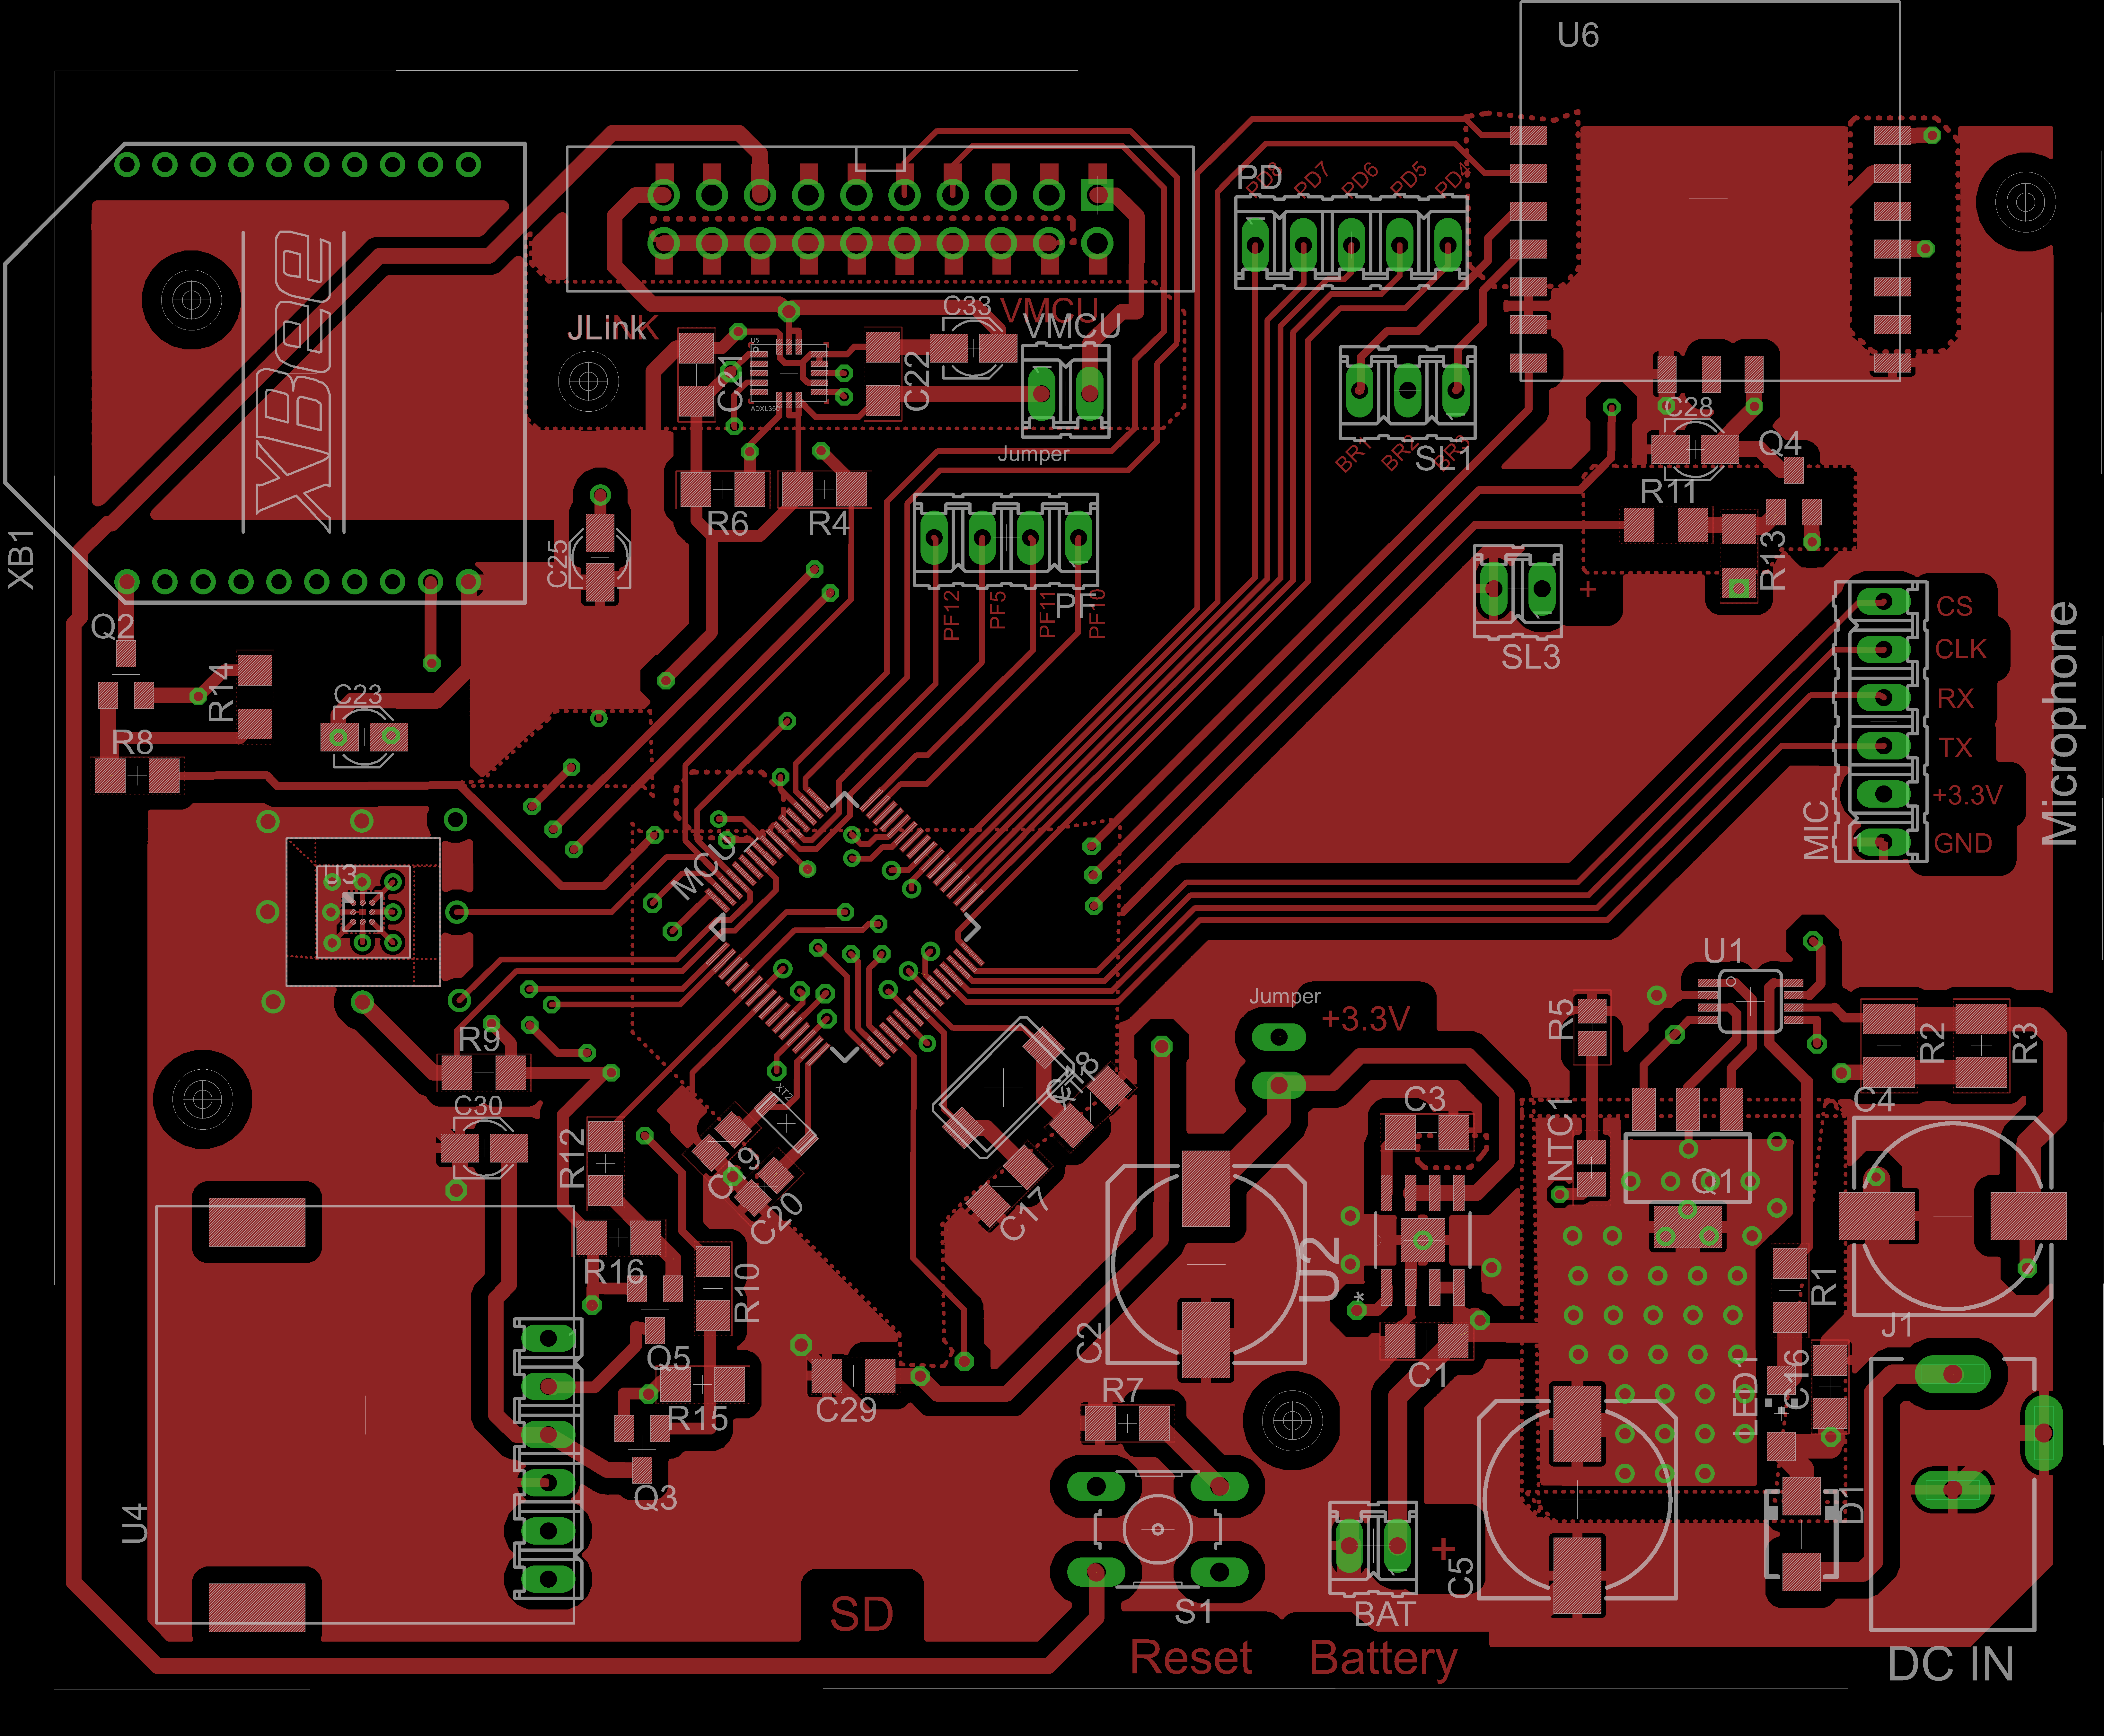
\includegraphics[width=\columnwidth]{Images/pcb_layout_top}
\caption{PCB layout top}
\label{fig:pcb_layout_top}
\end{figure}

\begin{figure}[htb]

\includegraphics[width=\columnwidth]{Images/dummy}
%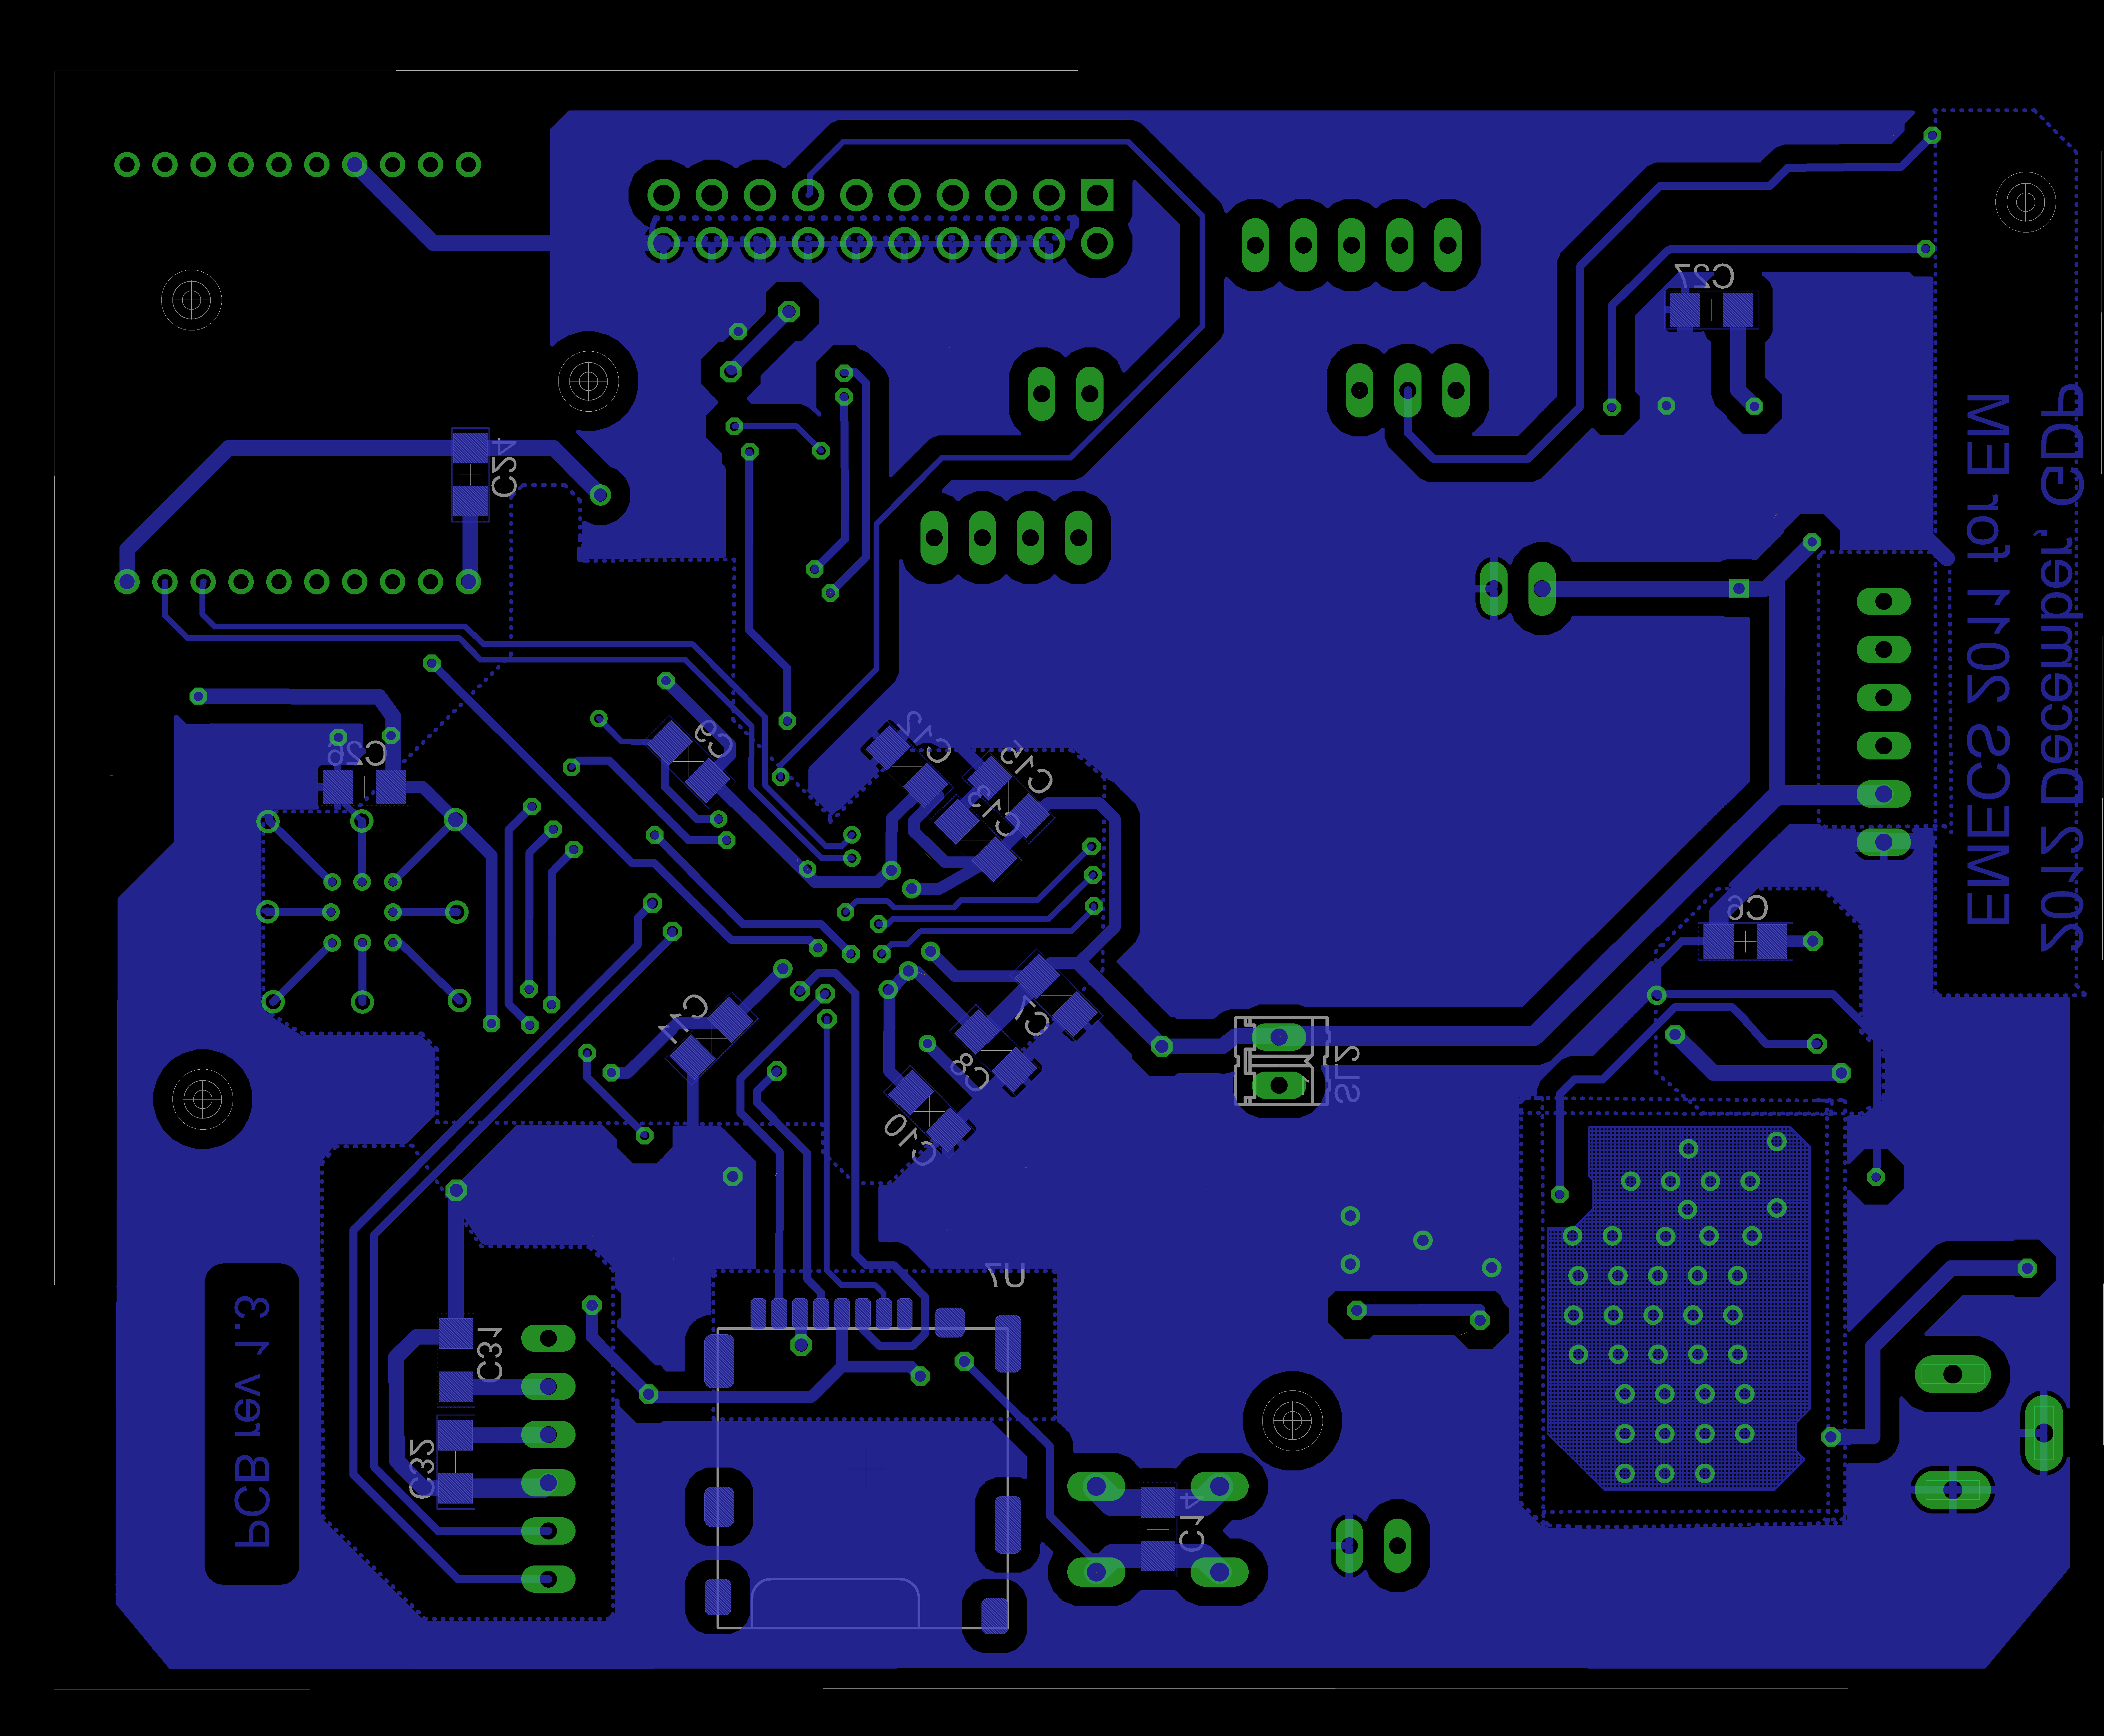
\includegraphics[width=\columnwidth]{Images/pcb_layout_bottom}
\caption{PCB layout bottom}
\label{fig:pcb_layout_bottom}
\end{figure}

\begin{figure}[htb]
\centering
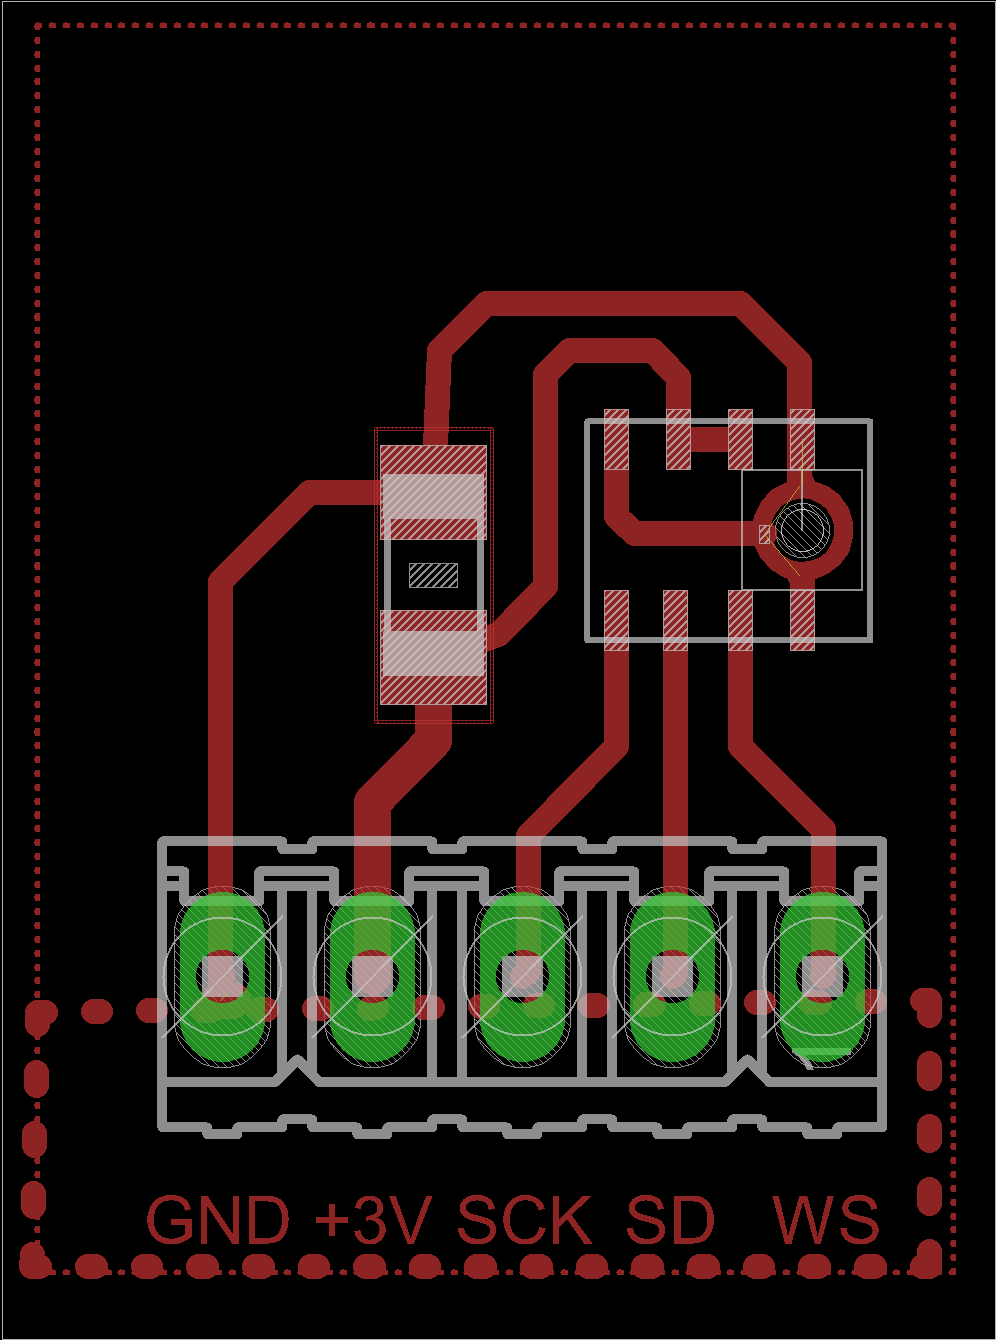
\includegraphics[width=0.4\columnwidth]{Images/pcb_layout_mic}
\caption{PCB layout microphone}
\label{fig:pcb_layout_mic}
\end{figure}

\clearpage

\section{PCB schematics}
\label{sec:pcb_schematics}
\begin{itemize}
\item PCB Schematics: ANT, XBee and SD \ref{fig:pcb_schematics_1}
\item PCB Schematics: Debug headers and microphone \ref{fig:pcb_schematics_2}
\item PCB Schematics: I2C and GPS \ref{fig:pcb_schematics_3}
\item PCB schematics: MCU, decoupling, oscillators and reset \ref{fig:pcb_schematics_4}
\item PCB schematics: Microphone \ref{fig:pcb_schematics_5}
\item PCB schematics: Power and LDO \ref{fig:pcb_schematics_6}
\end{itemize}

\begin{figure}[htb]
\centering
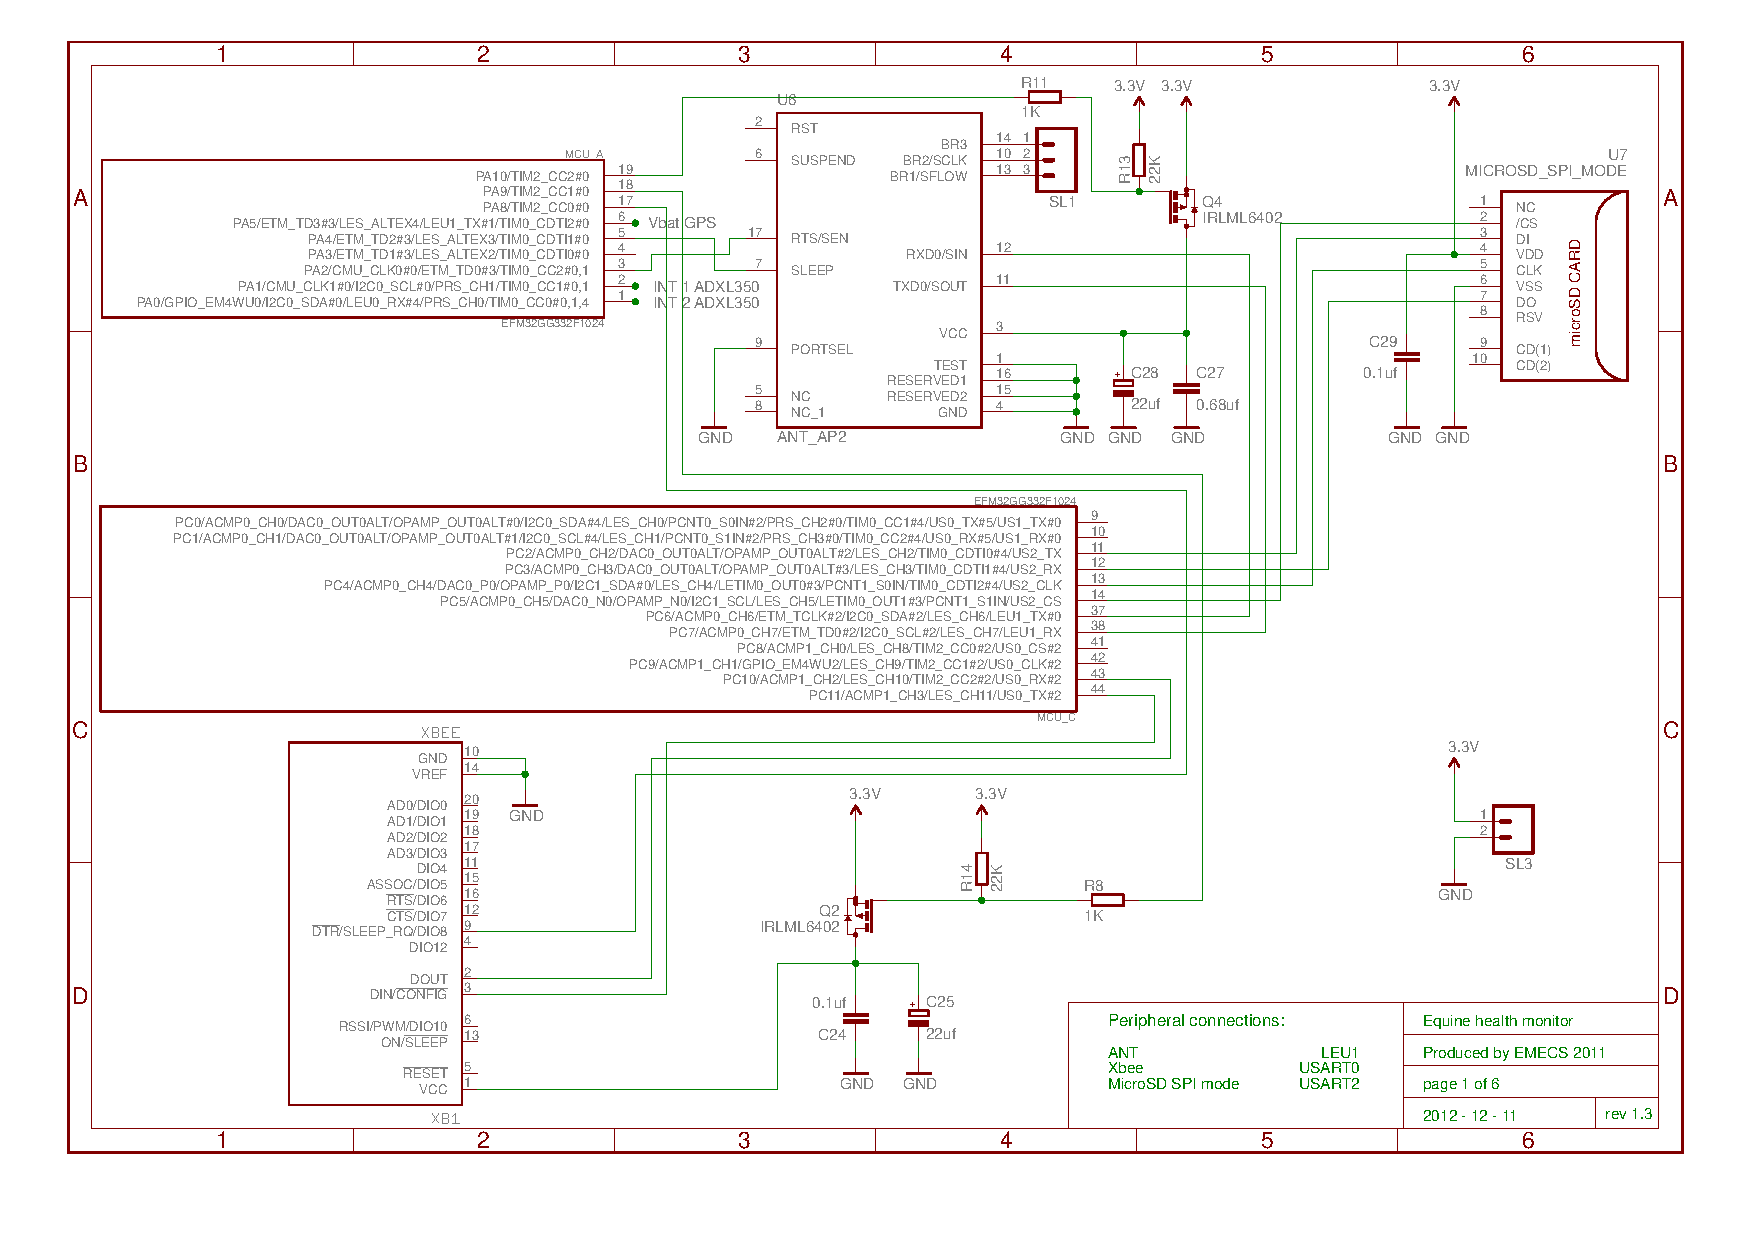
\includegraphics[width=\columnwidth]{Images/pcb_ant}
\caption{PCB schematics: ANT, XBee and SD}
\label{fig:pcb_schematics_1}
\end{figure}

\begin{figure}[htb]
\centering
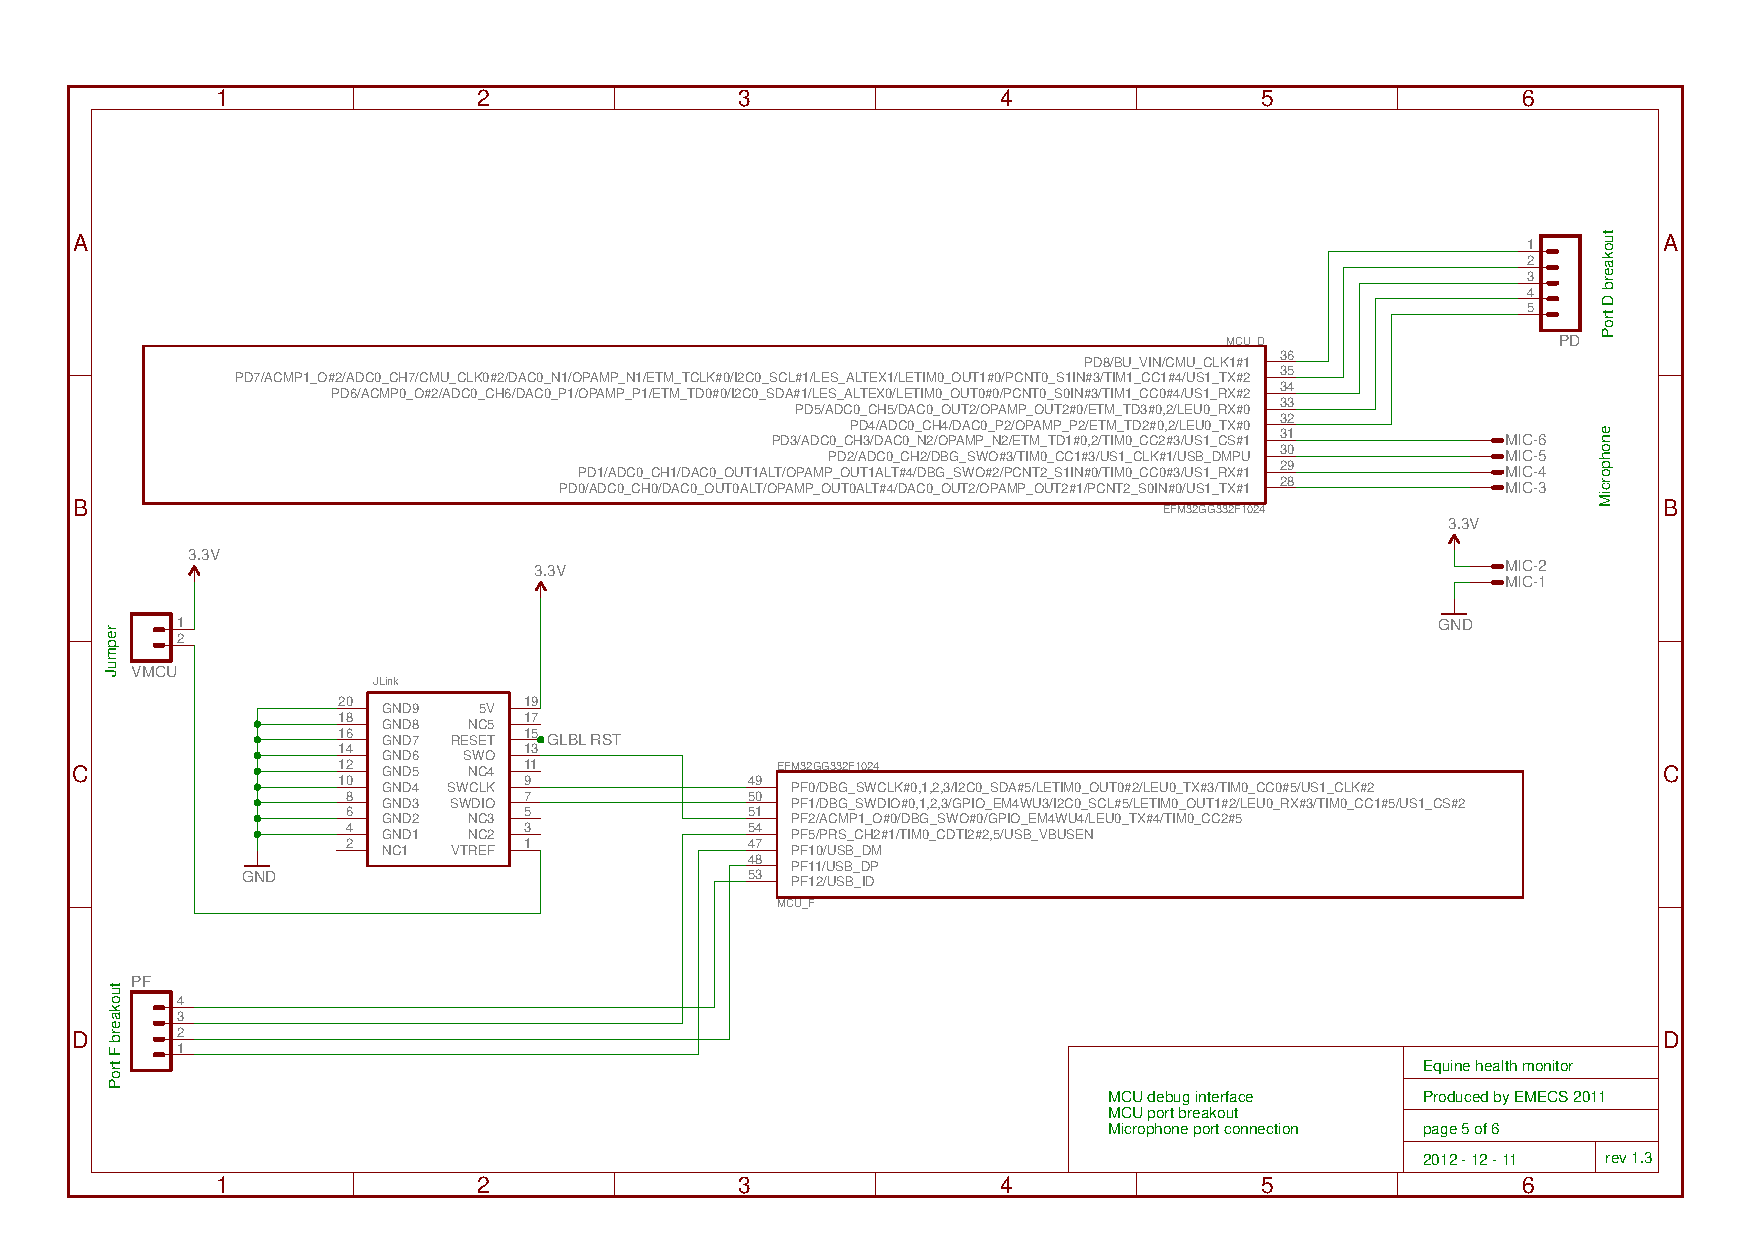
\includegraphics[width=\columnwidth]{Images/pcb_debug_mic}
\caption{PCB schematics: Debug headers and microphone}
\label{fig:pcb_schematics_2}
\end{figure}

\begin{figure}[htb]
\centering
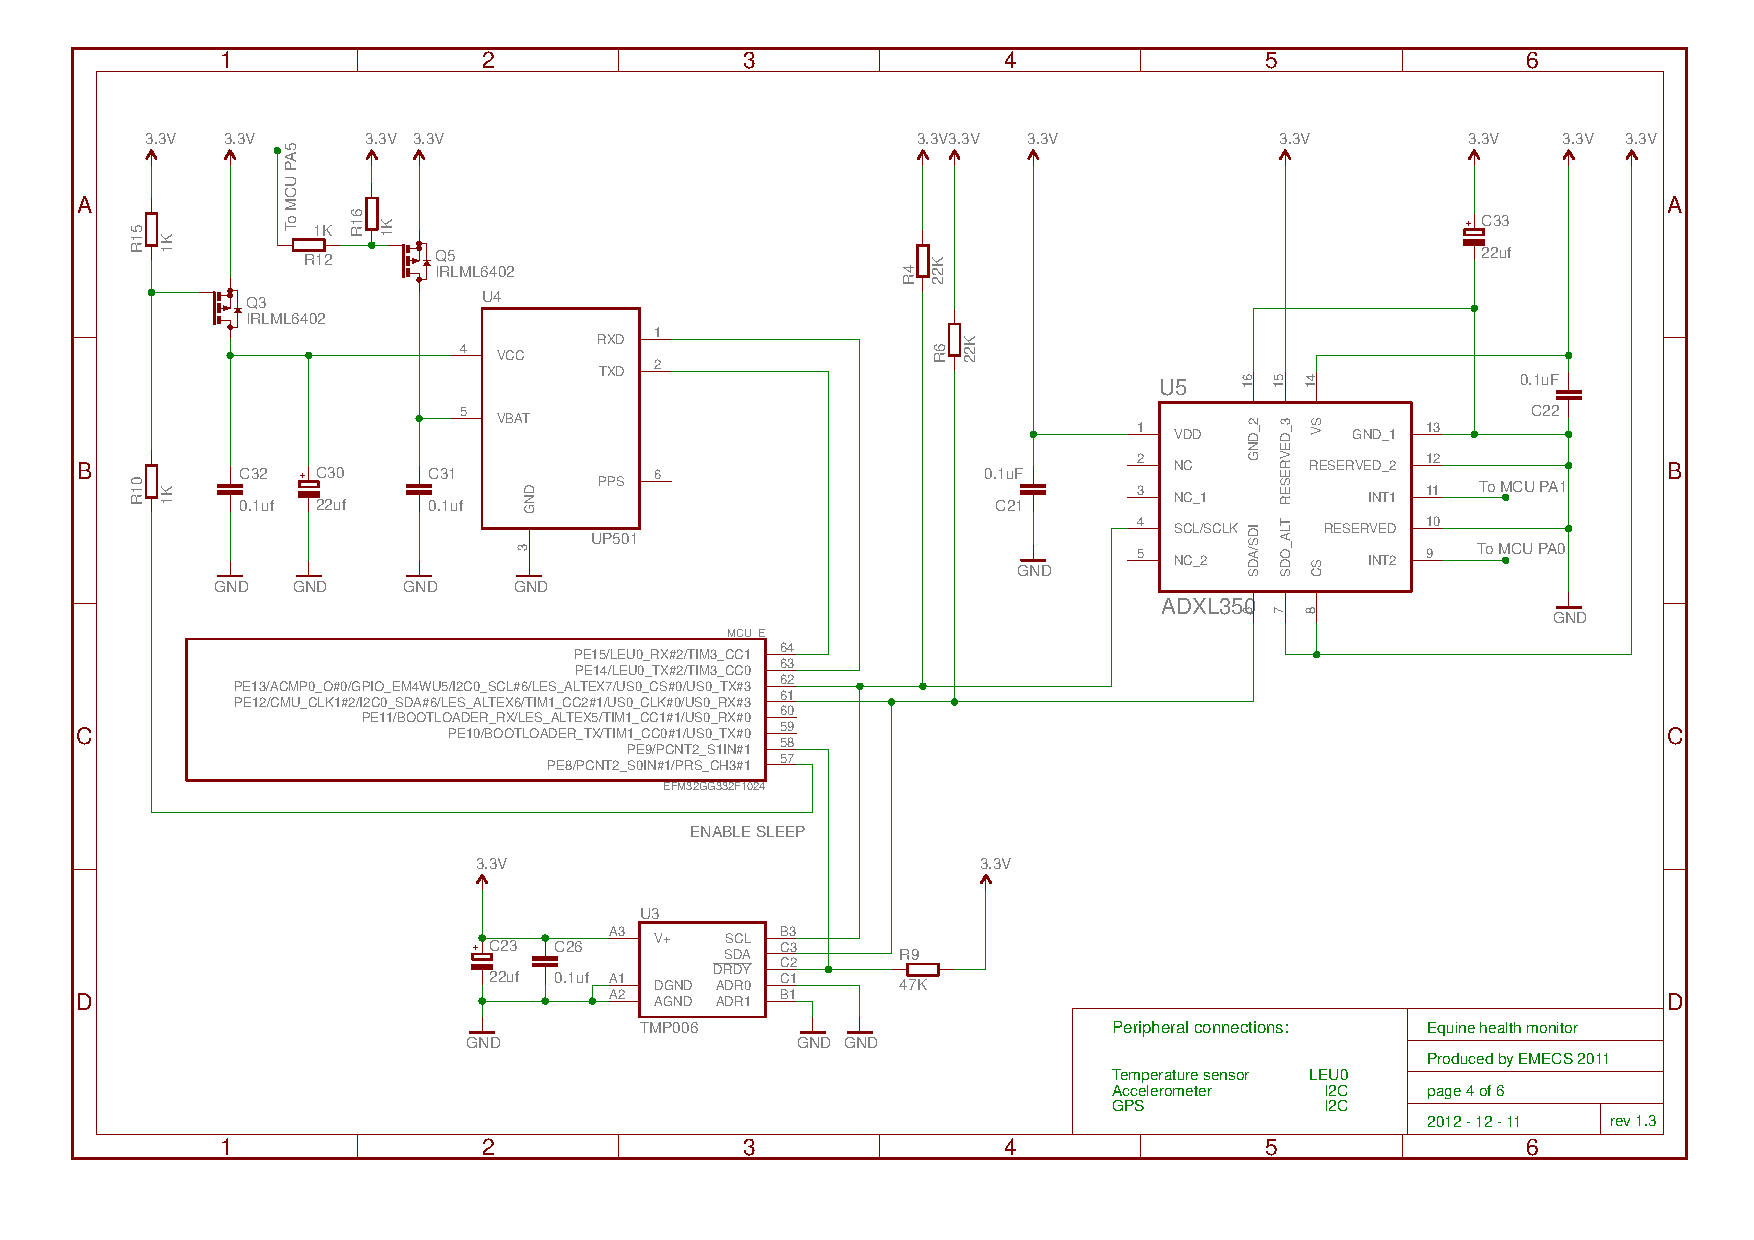
\includegraphics[width=\columnwidth]{Images/pcb_i2c_gps}
\caption{PCB schematics: I2C and GPS}
\label{fig:pcb_schematics_3}
\end{figure}

\begin{figure}[htb]
\centering
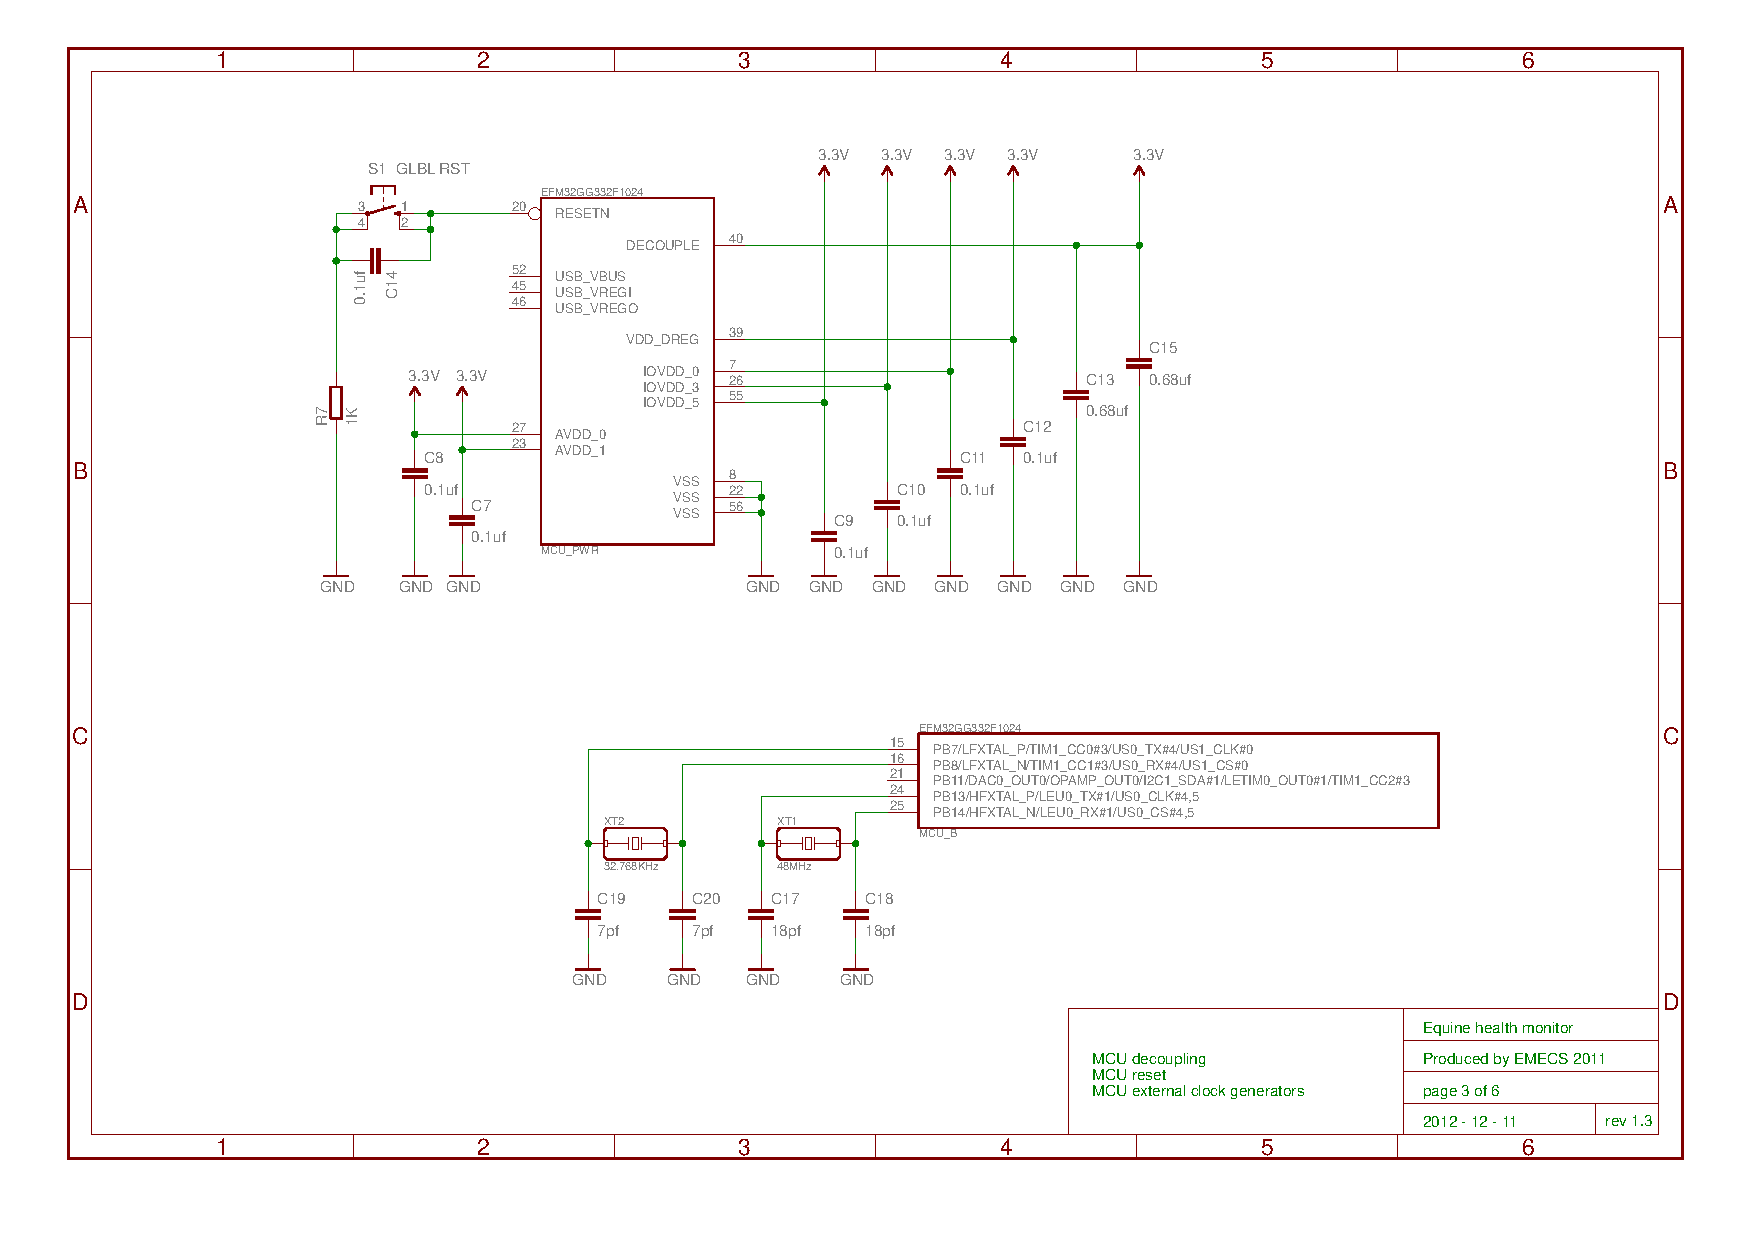
\includegraphics[width=\columnwidth]{Images/pcb_mcu_osc_reset}
\caption{PCB schematics: MCU, decoupling, oscillators and reset}
\label{fig:pcb_schematics_4}
\end{figure}

\begin{figure}[htb]
\centering
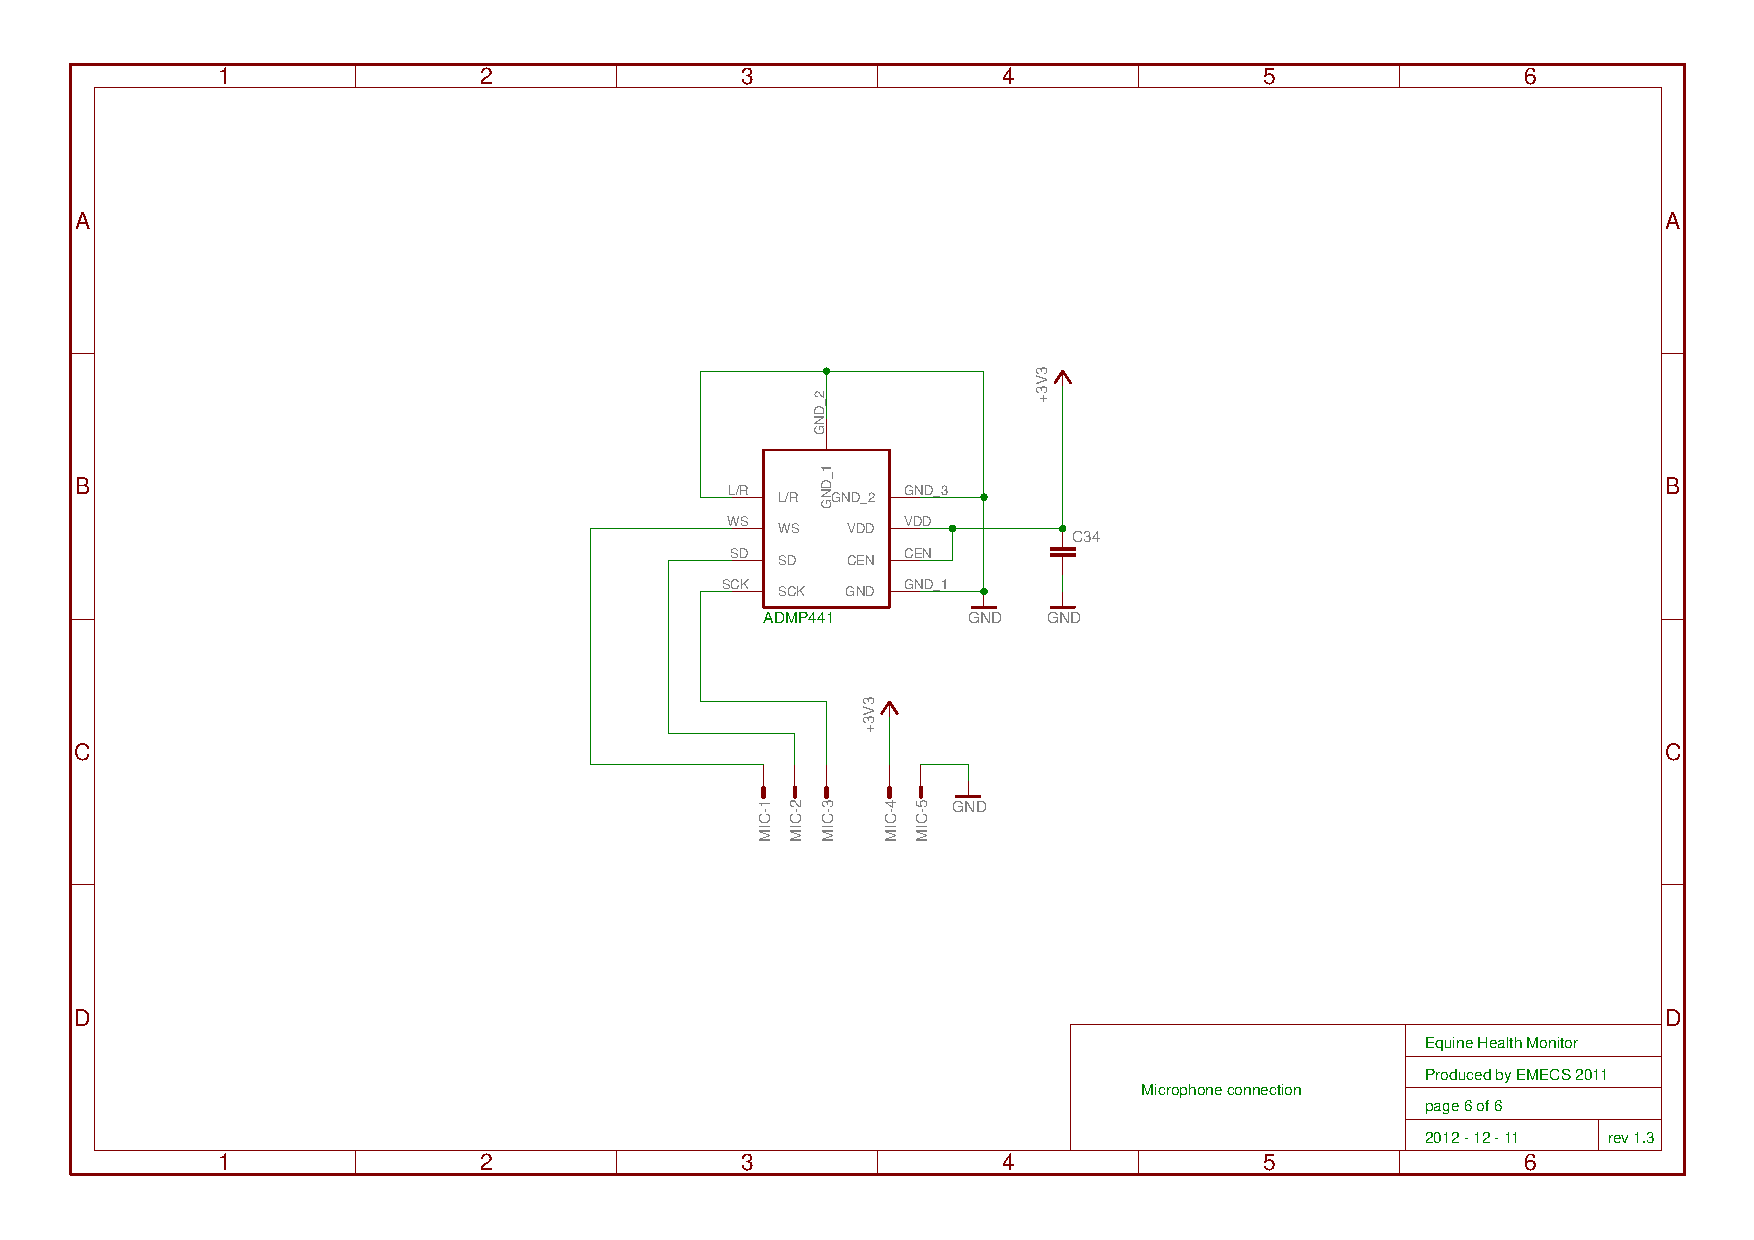
\includegraphics[width=\columnwidth]{Images/pcb_mic}
\caption{PCB schematics: Microphone}
\label{fig:pcb_schematics_5}
\end{figure}

\begin{figure}[htb]
\centering
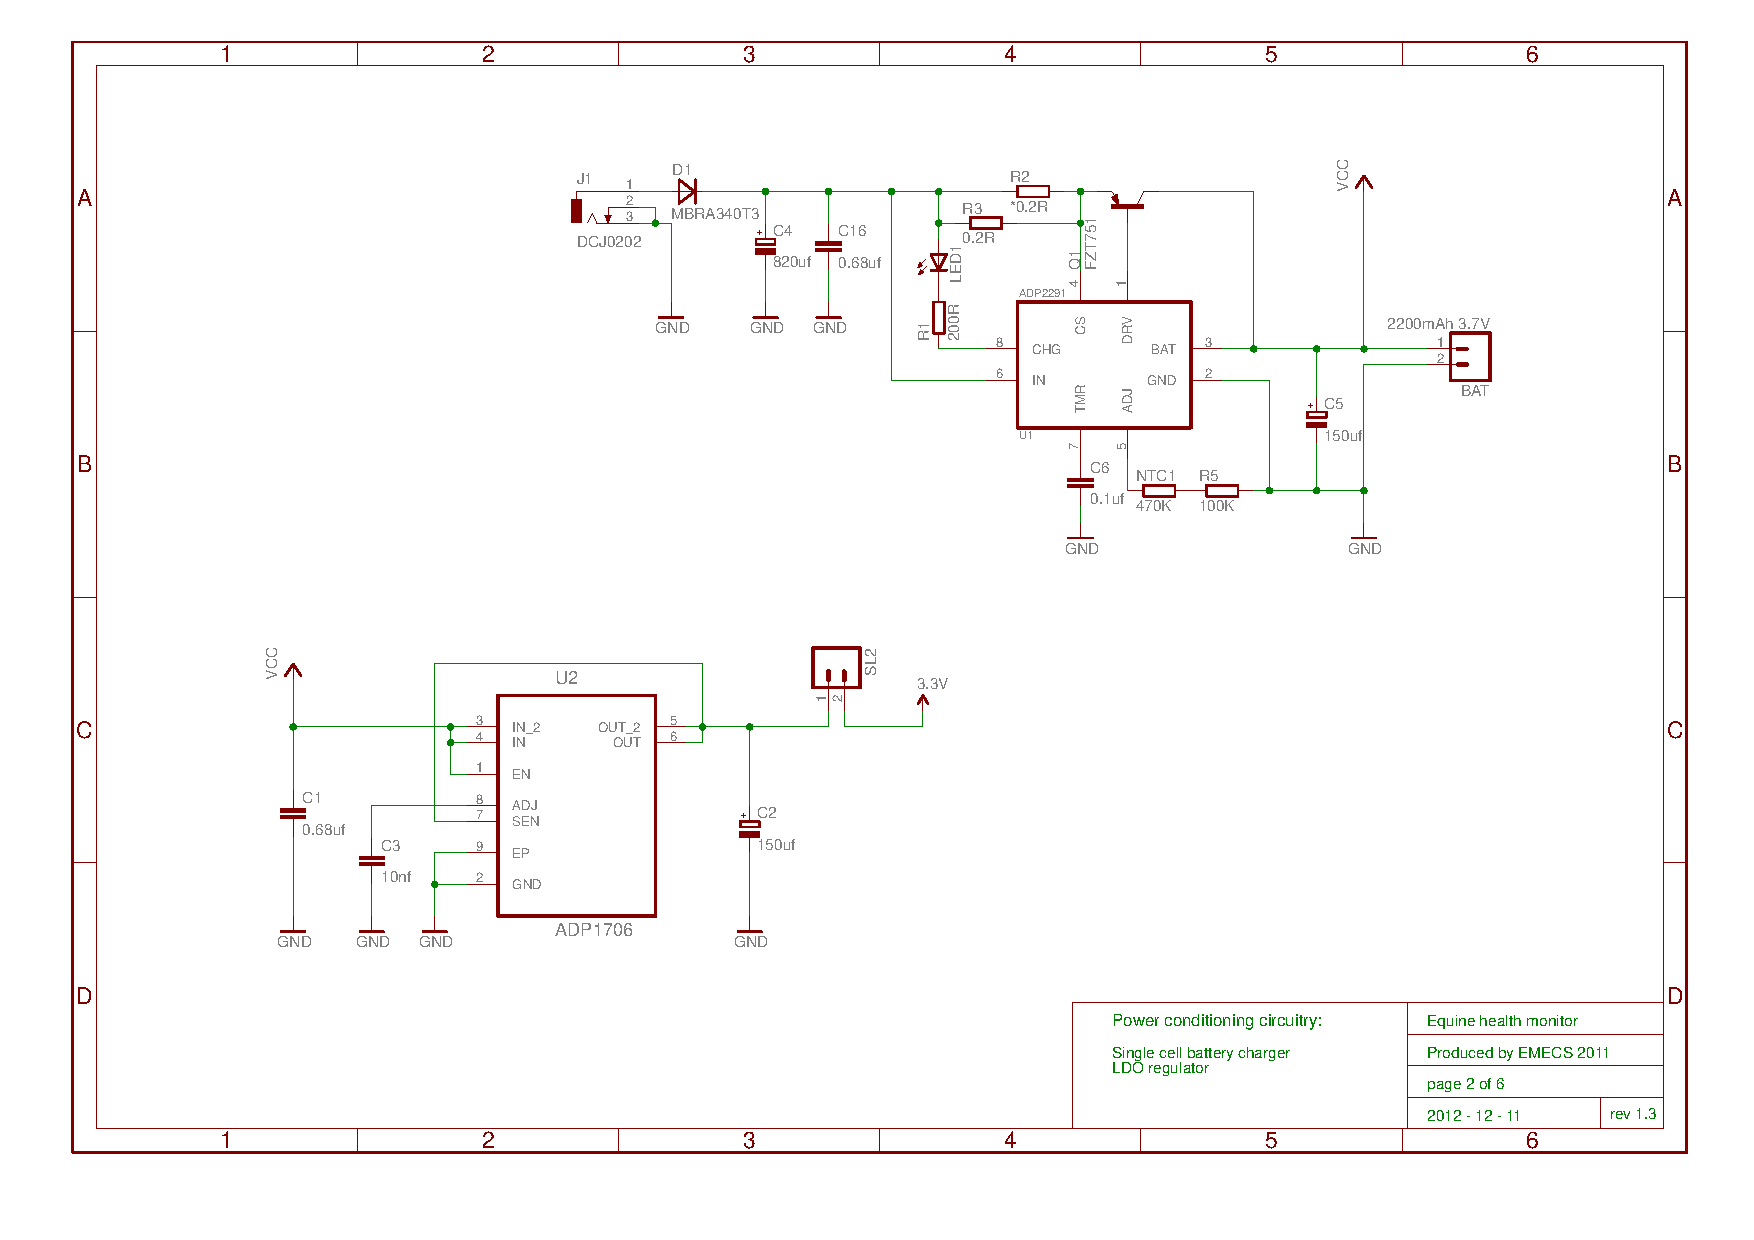
\includegraphics[width=\columnwidth]{Images/pcb_power_ldo}
\caption{PCB schematics: Power and LDO}
\label{fig:pcb_schematics_6}
\end{figure}




\clearpage
\section{Gantt Chart}
\label{sec:gantt_chart}
\begin{figure}[htb]
\centering
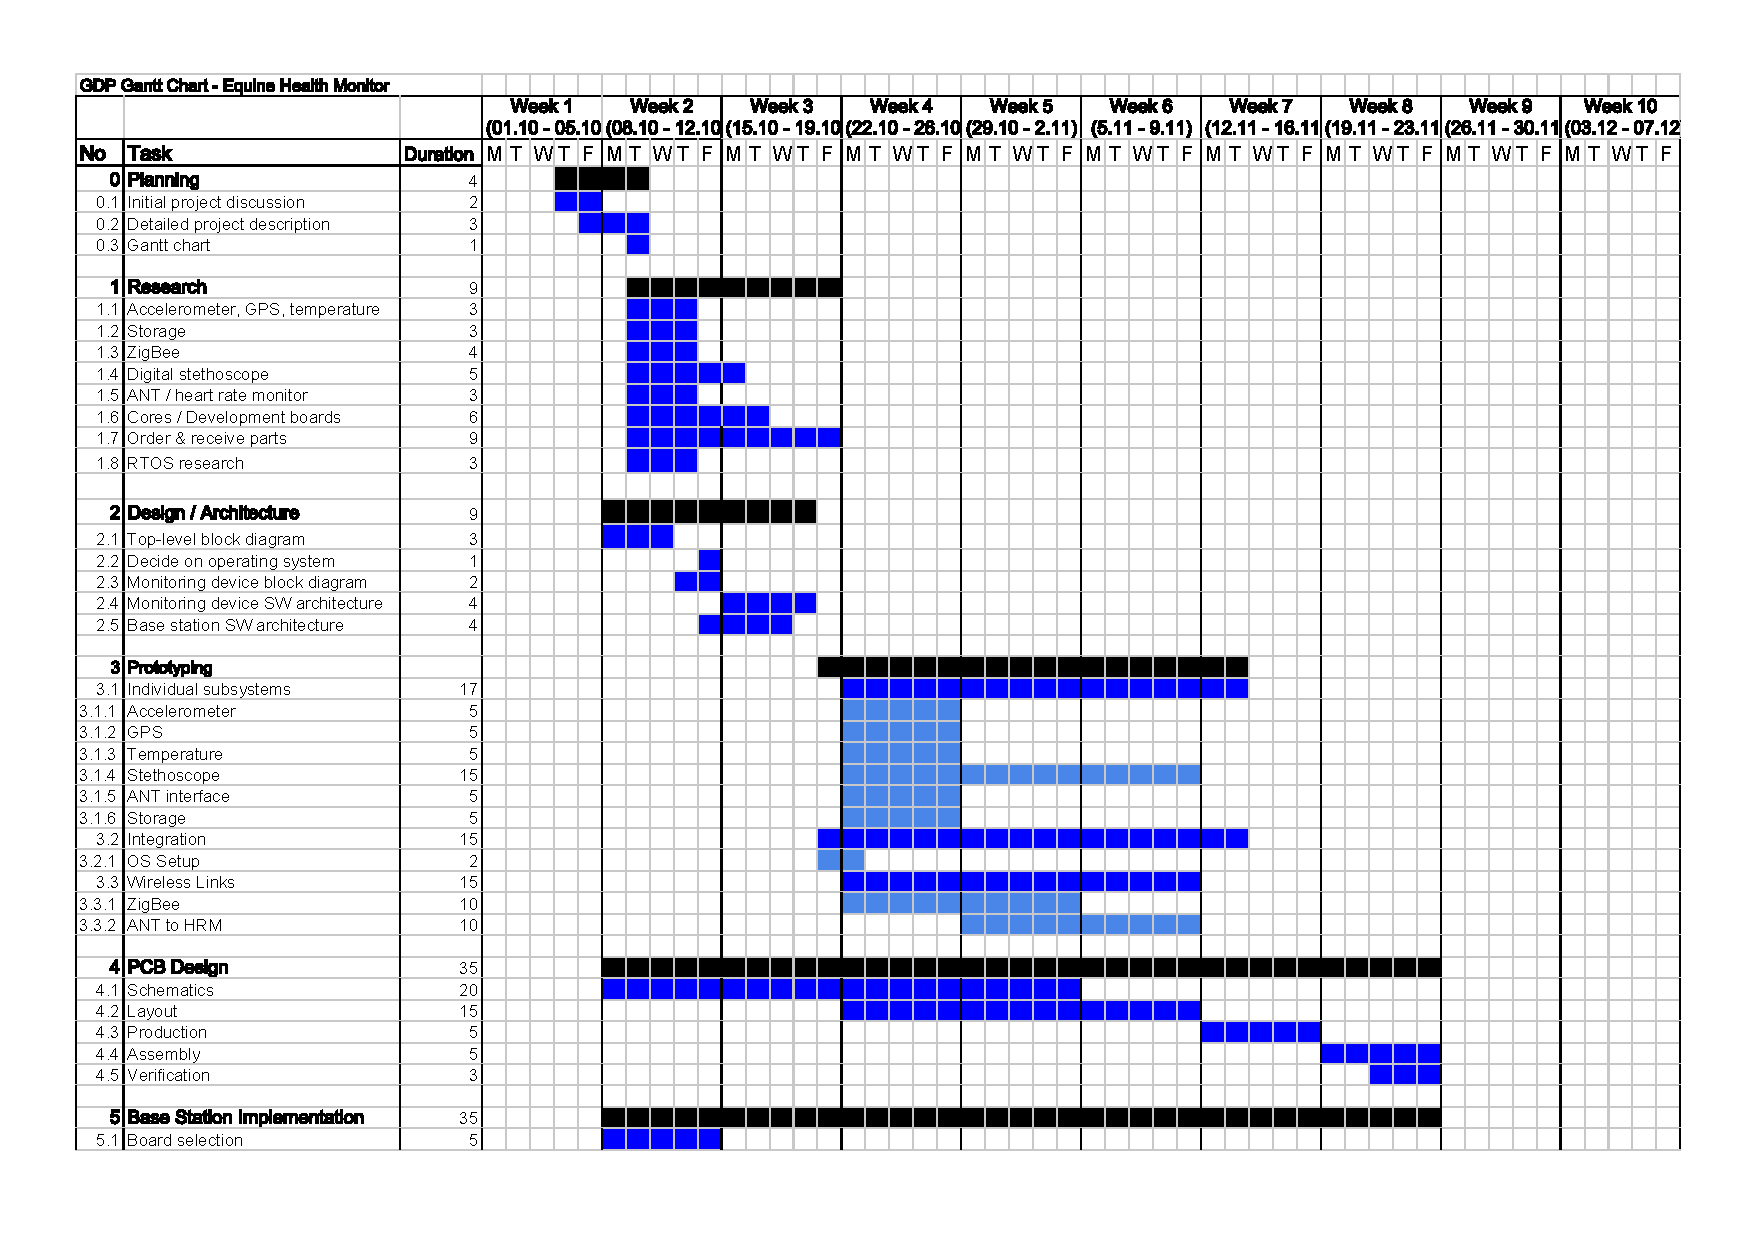
\includegraphics[angle=90, width=0.9\columnwidth]{Data/gantt_chart}
\caption{Gantt Chart}
\label{fig:gantt_chart}
\end{figure}

\clearpage

\section{Task distribution}
\label{sec:task_distribution}
\TODO{}


\section{Task break-down}
\label{sec:task_breakdown}
\TODO{}

\section{Code Listings}
\subsection{sensorinterface.h}
\label{list:sensor_interface}


\section{Price List}
\label{sec:price_list}
Please refer to table \ref{tab:pricelist}.
\begin{table}[hb]
\centering
\begin{tabular}{|l|l|l|}\hline%
\bfseries Component & \bfseries Price (GBP) & \bfseries Retail Price (GBP)\\\hline
\csvreader[ %
	head to column names,
	late after line=\\
]{Data/price_list.csv}{}%
{\Component & \Price & \Retail}%
\hline
\end{tabular}
\caption{Component Price List}
\label{tab:pricelist}
\end{table}
\clearpage

\section{Part List}
\label{sec:part_list}
Please refer to table \ref{tab:part_list_1} and \ref{tab:part_list_2} for the part list. 

\begin{sidewaystable}
\scriptsize
\begin{tabular}{|l|l|l|m{2.3cm}|l|l|l|}\hline%
\bfseries Part & \bfseries Value & \bfseries Device & \bfseries Description & \bfseries Package & \bfseries Manufacturer & \bfseries Man. part nr. \\\hline
\csvreader[ %
	head to column names,
	late after line=\\
]{Data/partlist_part1.csv}{}%
{\Part & \Value & \Device & \Description & \Package & \Manufacturer & \PartNr}%
\hline
\end{tabular}
\caption{Part list part 1}
\label{tab:part_list_1}
\end{sidewaystable}

\begin{sidewaystable}
\scriptsize
\begin{tabular}{|l|l|l|m{2.3cm}|l|l|l|}\hline%
\bfseries Part & \bfseries Value & \bfseries Device & \bfseries Description & \bfseries Package & \bfseries Manufacturer & \bfseries Man. part Nr. \\\hline
\csvreader[head to column names,
late after line=\\
]{Data/partlist_part2.csv}{}%
{\Part & \Value & \Device & \Description & \Package & \Manufacturer & \PartNr}%
\hline
\end{tabular}
\caption{Part list part 2}
\label{tab:part_list_2}
\end{sidewaystable}
\clearpage

\section{Fieldtrip}
\subsection{Gut Sound Recordings}
\label{sec:gut_sound_recordings}
Please refer to table \ref{tab:gut_sound_recordings}
\begin{table}
\centering
\small
\begin{tabular}{|c|l|p{2cm}|l|}\hline%
\bfseries \# & \bfseries Description & \bfseries Part of the abdomen & \bfseries Link \\\hline
\csvreader[head to column names,
late after line=\\
]{Data/gut_sound_recordings.csv}{}%
{\Horse & \Type & \Part & \Link}%
\hline
\end{tabular}
\caption{Gut sound recordings}
\label{tab:gut_sound_recordings}
\end{table}


\subsection{Pictures}
Please refer to figure \ref{fig:field_trip_a} and \ref{fig:field_trip_b}.
\begin{figure}[htb]
\centering
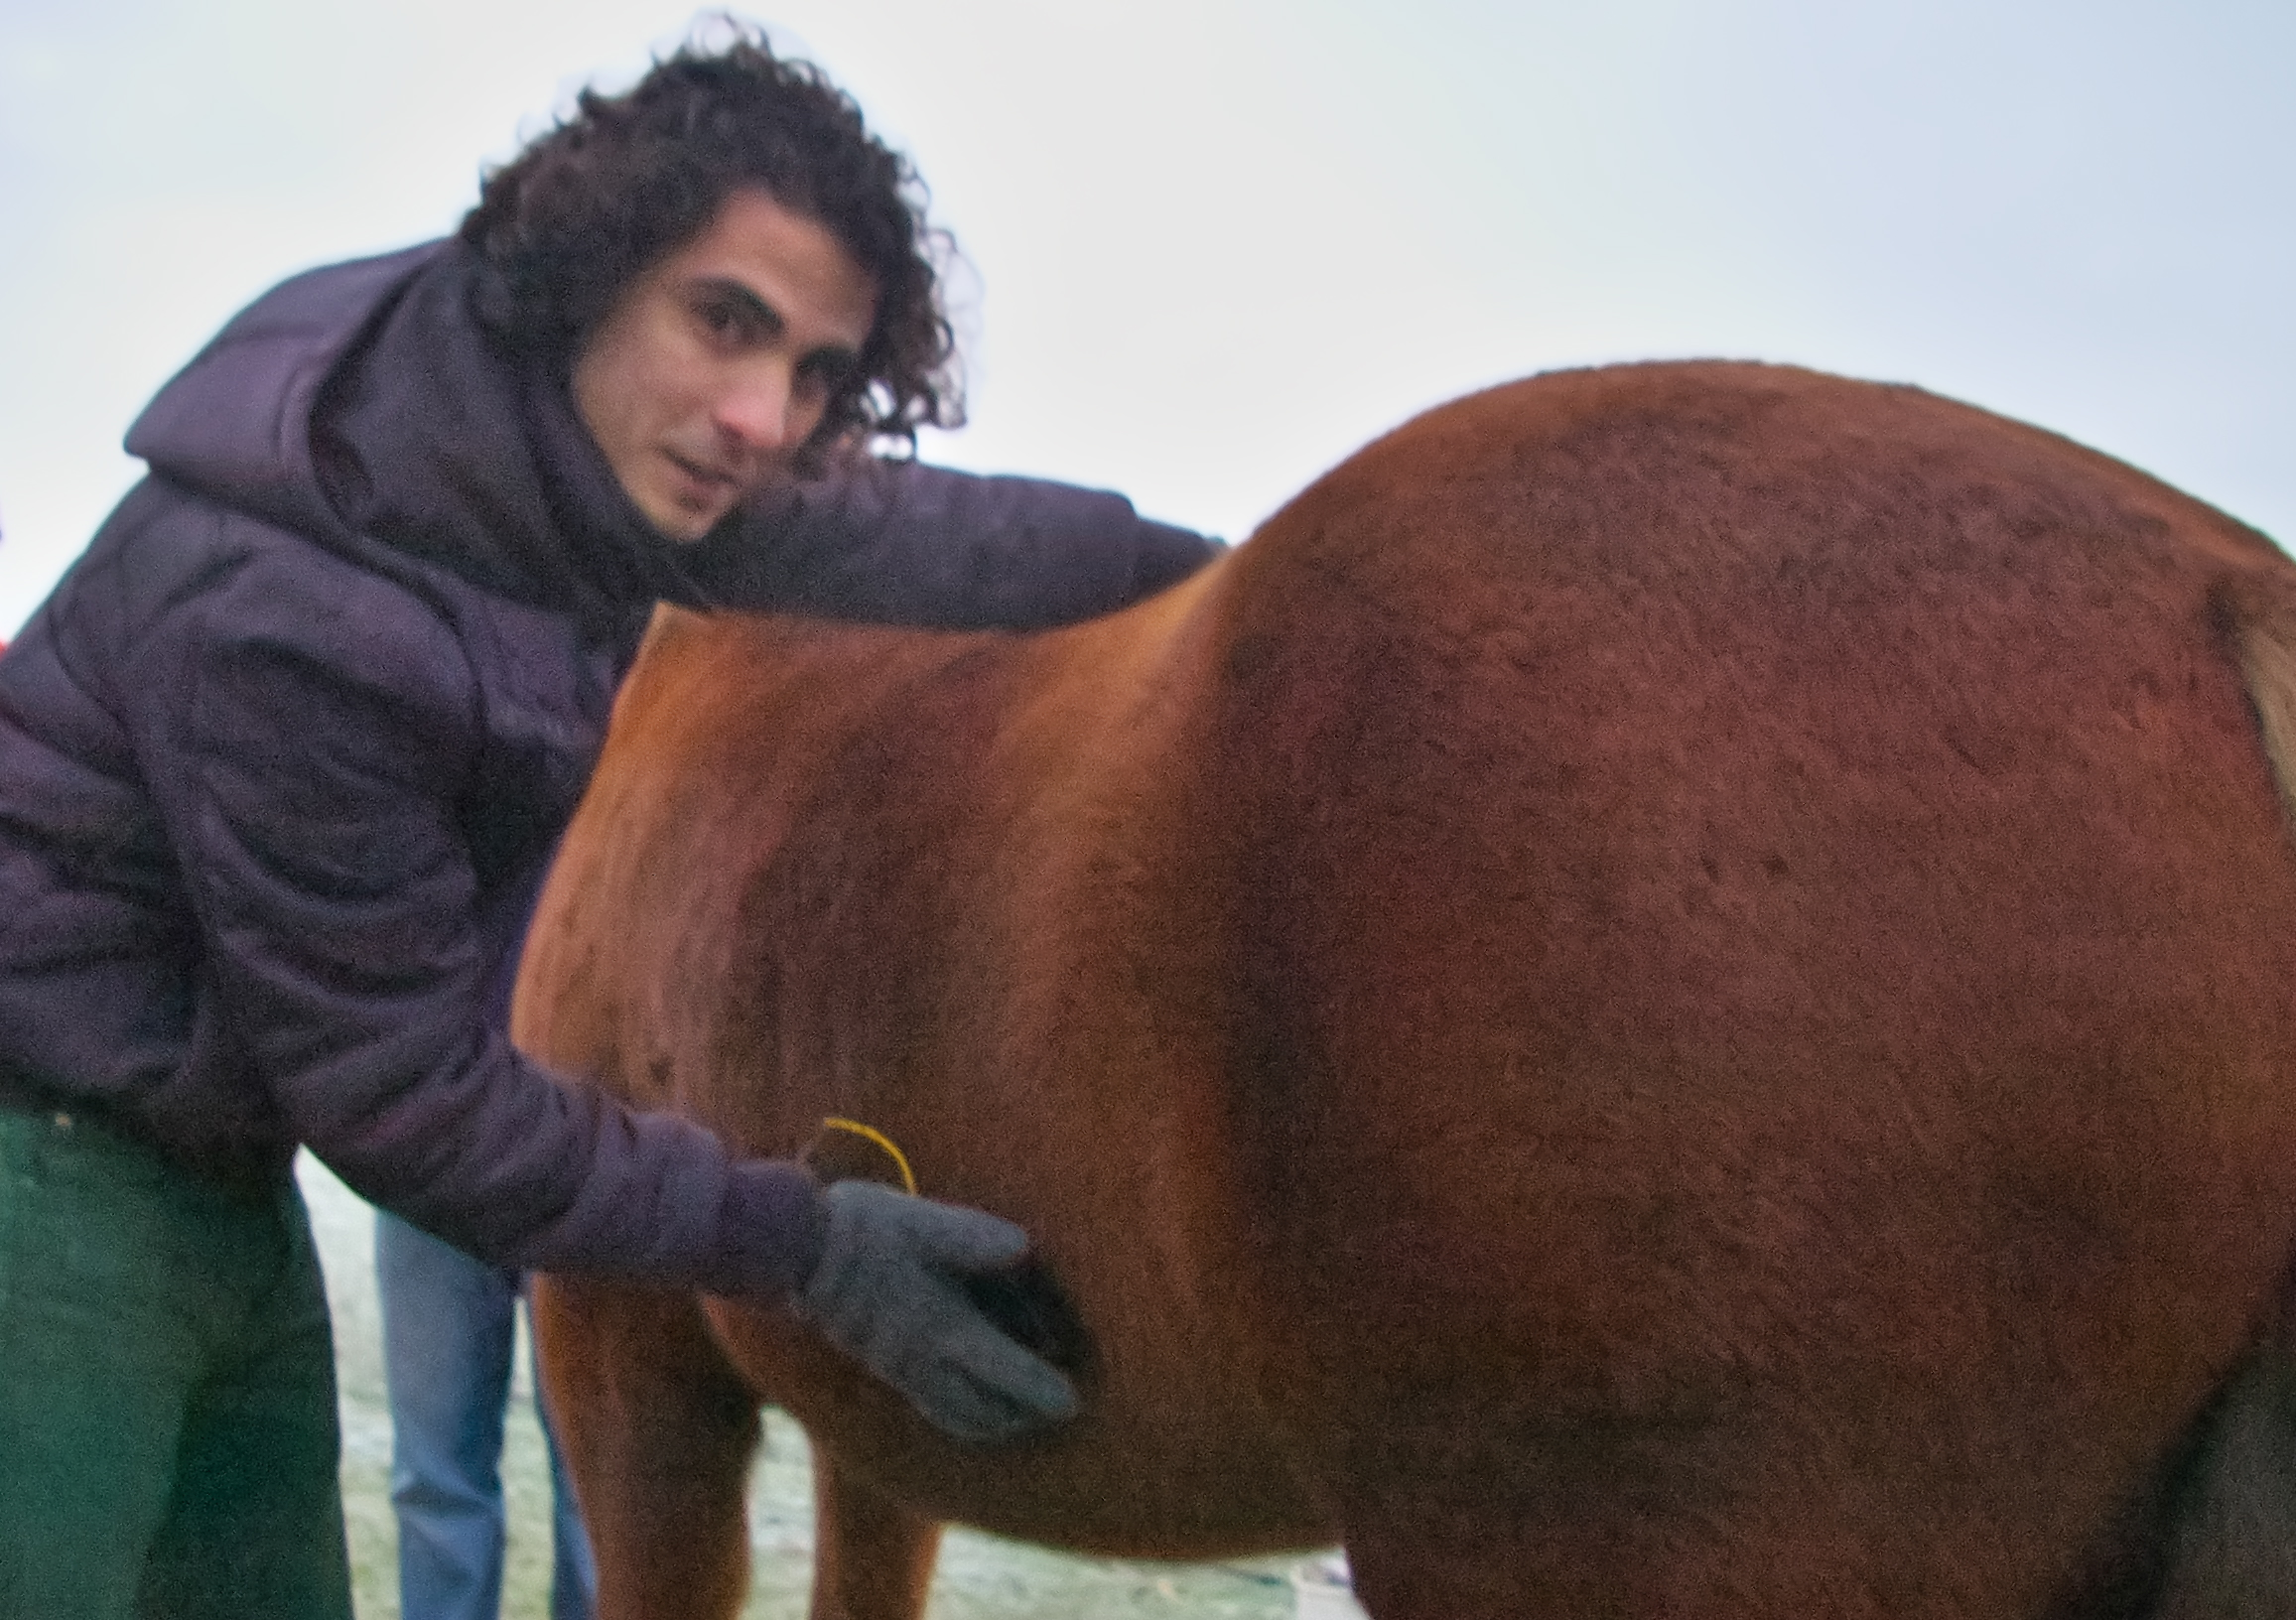
\includegraphics[width=0.7\columnwidth]{Images/field_trip_a.jpg}
\caption{Photo: Field trip (a)}
\label{fig:field_trip_a}
\end{figure}
\begin{figure}[htb]
\centering
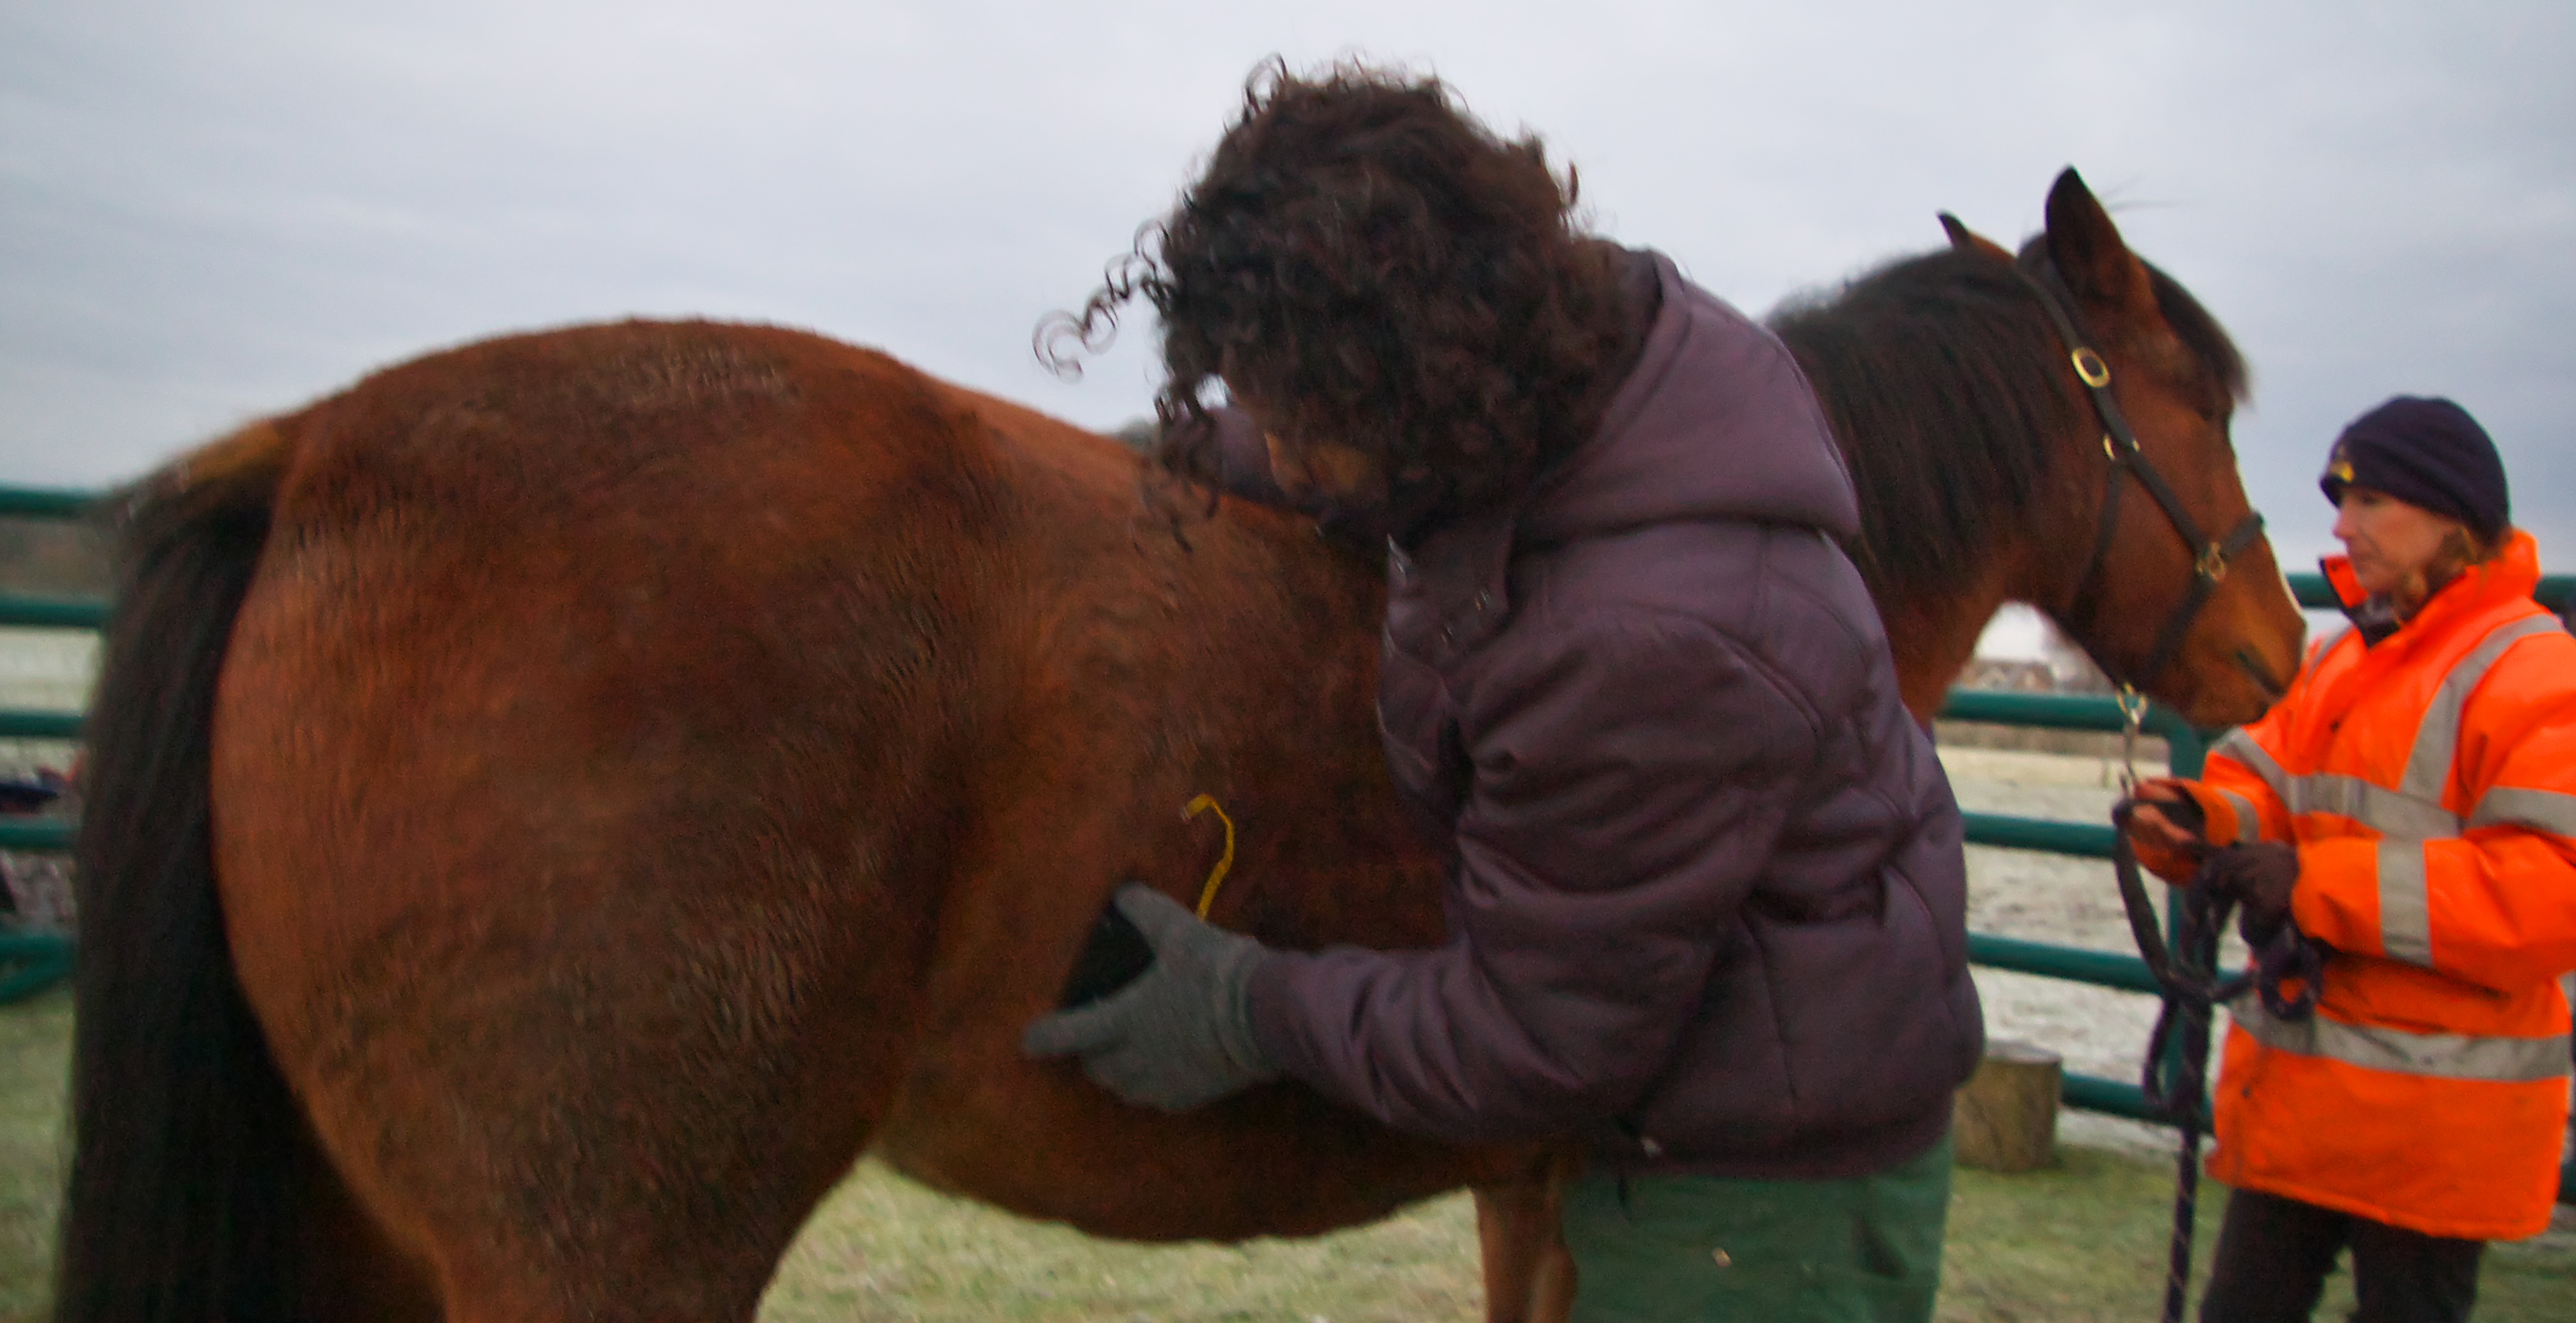
\includegraphics[width=0.7\columnwidth]{Images/field_trip_b.jpg}
\caption{Photo: Field trip (b)}
\label{fig:field_trip_b}
\end{figure}


\clearpage


%--------------Credits----------------------------
\bibliographystyle{ecs}
\bibliography{references}	% print the biblography
\addcontentsline{toc}{chapter}{Bibliography}
\end{document}
